\documentclass{article}

% packages
  % basic stuff for rendering math
  \usepackage[letterpaper, top=1in, bottom=1in, left=1in, right=1in]{geometry}
  \usepackage[utf8]{inputenc}
  \usepackage[english]{babel}
  \usepackage{amsmath} 
  \usepackage{amssymb}
  % \usepackage{amsthm}

  % extra math symbols and utilities
  \usepackage{mathtools}        % for extra stuff like \coloneqq
  \usepackage{mathrsfs}         % for extra stuff like \mathsrc{}
  \usepackage{centernot}        % for the centernot arrow 
  \usepackage{bm}               % for better boldsymbol/mathbf 
  \usepackage{enumitem}         % better control over enumerate, itemize
  \usepackage{hyperref}         % for hypertext linking
  \usepackage{fancyvrb}          % for better verbatim environments
  \usepackage{newverbs}         % for texttt{}
  \usepackage{xcolor}           % for colored text 
  \usepackage{listings}
  \usepackage{lstautogobble}
  \usepackage{parcolumns}

  \usepackage[T1]{fontenc}

  % page layout
  \usepackage{fancyhdr}         % for headers and footers 
  \usepackage{lastpage}         % to include last page number in footer 
  \usepackage{parskip}          % for no indentation and space between paragraphs    


  % for custom environments
  \usepackage{tcolorbox}        % for better colored boxes in custom environments
  \tcbuselibrary{breakable}     % to allow tcolorboxes to break across pages

  % figures
  \usepackage{pgfplots}
  \pgfplotsset{compat=1.18}
  \usepackage{float}            % for [H] figure placement
  \usepackage{tikz}
  \usepackage{tikz-cd}
  % \usepackage{circuit-tikz}
  \usetikzlibrary{arrows}
  \usetikzlibrary{positioning}
  \usetikzlibrary{calc}
  \usepackage{graphicx}
  \usepackage{caption} 
  \usepackage{subcaption}
  \captionsetup{font=small}

  % for tabular stuff 
  \usepackage{dcolumn}

  \usepackage[nottoc]{tocbibind}
  \pdfsuppresswarningpagegroup=1
  \hfuzz=5.002pt                % ignore overfull hbox badness warnings below this limit

% New and replaced operators
  \DeclareMathOperator{\Tr}{Tr}
  \DeclareMathOperator{\Sym}{Sym}
  \DeclareMathOperator{\Span}{span}
  \DeclareMathOperator{\std}{std}
  \DeclareMathOperator{\Cov}{Cov}
  \DeclareMathOperator{\Var}{Var}
  \DeclareMathOperator{\Corr}{Corr}
  \DeclareMathOperator{\pos}{pos}
  \DeclareMathOperator*{\argmin}{\arg\!\min}
  \DeclareMathOperator*{\argmax}{\arg\!\max}
  \newcommand{\ket}[1]{\ensuremath{\left|#1\right\rangle}}
  \newcommand{\bra}[1]{\ensuremath{\left\langle#1\right|}}
  \newcommand{\braket}[2]{\langle #1 | #2 \rangle}
  \newcommand{\qed}{\hfill$\blacksquare$}     % I like QED squares to be black

% Custom Environments
  \newtcolorbox[auto counter, number within=section]{question}[1][]
  {
    colframe = orange!25,
    colback  = orange!10,
    coltitle = orange!20!black,  
    breakable, 
    title = \textbf{Question \thetcbcounter ~(#1)}
  }

  \newtcolorbox[auto counter, number within=section]{exercise}[1][]
  {
    colframe = teal!25,
    colback  = teal!10,
    coltitle = teal!20!black,  
    breakable, 
    title = \textbf{Exercise \thetcbcounter ~(#1)}
  }
  \newtcolorbox[auto counter, number within=section]{solution}[1][]
  {
    colframe = violet!25,
    colback  = violet!10,
    coltitle = violet!20!black,  
    breakable, 
    title = \textbf{Solution \thetcbcounter}
  }
  \newtcolorbox[auto counter, number within=section]{lemma}[1][]
  {
    colframe = red!25,
    colback  = red!10,
    coltitle = red!20!black,  
    breakable, 
    title = \textbf{Lemma \thetcbcounter ~(#1)}
  }
  \newtcolorbox[auto counter, number within=section]{theorem}[1][]
  {
    colframe = red!25,
    colback  = red!10,
    coltitle = red!20!black,  
    breakable, 
    title = \textbf{Theorem \thetcbcounter ~(#1)}
  } 
  \newtcolorbox[auto counter, number within=section]{proof}[1][]
  {
    colframe = orange!25,
    colback  = orange!10,
    coltitle = orange!20!black,  
    breakable, 
    title = \textbf{Proof. }
  } 
  \newtcolorbox[auto counter, number within=section]{definition}[1][]
  {
    colframe = yellow!25,
    colback  = yellow!10,
    coltitle = yellow!20!black,  
    breakable, 
    title = \textbf{Definition \thetcbcounter ~(#1)}
  } 
  \newtcolorbox[auto counter, number within=section]{example}[1][]
  {
    colframe = blue!25,
    colback  = blue!10,
    coltitle = blue!20!black,  
    breakable, 
    title = \textbf{Example \thetcbcounter ~(#1)}
  } 
  \newtcolorbox[auto counter, number within=section]{code}[1][]
  {
    colframe = green!25,
    colback  = green!10,
    coltitle = green!20!black,  
    breakable, 
    title = \textbf{Code \thetcbcounter ~(#1)}
  } 
  \definecolor{dkgreen}{rgb}{0,0.6,0}
  \definecolor{gray}{rgb}{0.5,0.5,0.5}
  \definecolor{mauve}{rgb}{0.58,0,0.82}
  \definecolor{lightgray}{gray}{0.93}
  \lstset{
    autogobble,
    frame=ltbr,
    language=C,
    aboveskip=3mm,
    belowskip=3mm,
    showstringspaces=false,
    columns=fullflexible,
    keepspaces=true,
    basicstyle={\small\ttfamily},
    numbers=left,
    firstnumber=1, 
    numberstyle=\tiny\color{gray},
    keywordstyle=\color{blue},
    commentstyle=\color{dkgreen},
    stringstyle=\color{mauve},
    backgroundcolor=\color{lightgray}, 
    breaklines=true,
    breakatwhitespace=true,
    tabsize=3, 
    xleftmargin=2em, 
    framexleftmargin=1.5em, 
    stepnumber=1
  }

% Page style
  \pagestyle{fancy}
  \fancyhead[L]{}
  \fancyhead[C]{Muchang Bahng}
  \fancyhead[R]{Spring 2024} 
  \fancyfoot[C]{\thepage / \pageref{LastPage}}
  \renewcommand{\footrulewidth}{0.4pt}          % the footer line should be 0.4pt wide
  \renewcommand{\thispagestyle}[1]{}  % needed to include headers in title page

\begin{document}

\title{Computer Systems}
\author{Muchang Bahng}
\date{Spring 2024}

\maketitle
\tableofcontents
\pagebreak

Before we do any coding, we must learn the theory behind how computer systems work, which all starts from memory management and CPU architecture. We will use C with the gcc compiler, along with MIPS and NASM assembler. It is imperative to learn these two since given that you know a high level language pretty well (Python in my case), you want to learn C to appreciate the things Python does for you, and you want to learn Assembly to appreciate the things C does for you.\footnote{https://www.youtube.com/watch?v=XlvfHOrF26M}. 

To start off, we want a big overall picture of high a computer works. We introduce this with the simplest model of the computer, the Von Nuemann architecture. It consists of a \textbf{central processing unit} (CPU), \textbf{memory}, and an \textbf{input/output} (I/O) system. We show a diagram of this first for conciseness in Figure \ref{fig:von_neumann_arch}. 

\begin{figure}[H]
  \centering 
  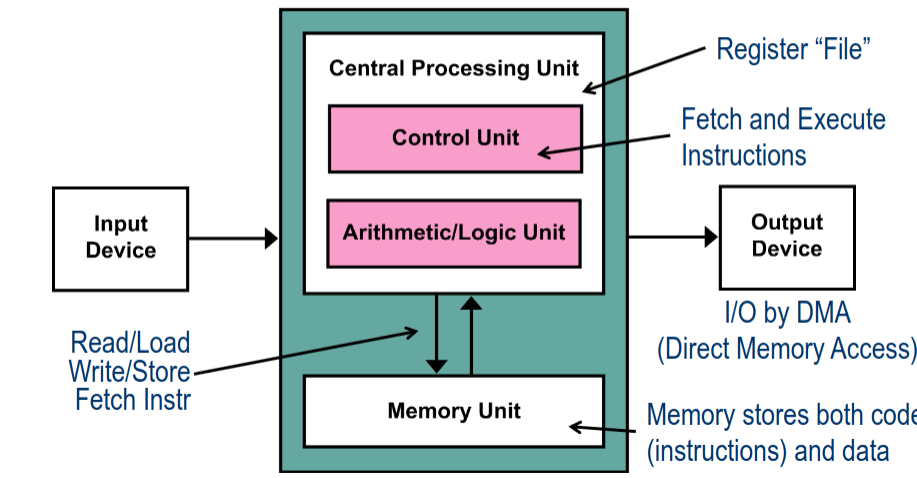
\includegraphics[scale=0.4]{img/von_neumann_arch.png}
  \caption{von Neumann Architecture} 
  \label{fig:von_neumann_arch}
\end{figure}

We will go through these one by one, touching on C and Assembly along the way, but the implementation of these things can differ by the \textbf{computer architecture}, so let's list some of the basic ones. 

\begin{definition}[Computer Architecture]
  The \textbf{computer architecture} is the design of the computer, which includes the CPU, memory, and I/O system. There are many different architectures, but we will focus on the most common ones.
\end{definition}

We first go over some basic theoretical properties of basic data types, focusing on C, and then we cover all the stuff about memory and then all the stuff about the CPU. This is a natural progression since to work with data, you must first know where to store the data and how it is stored (the memory), and then you want to know how data is manipulated (the CPU). 

\section{Primitive Types}

  Let's first define some basic terms. 

  \begin{definition}[Collections of Bits]
    There are many words that are used to talk about values of different data types: 
    \begin{enumerate}
      \item A \textbf{bit} (b) is either $0$ or $1$. 
      \item A \textbf{Hex} (x) is a collection of 4 bits, with a total of $2^4 = 16$ possible values, and this is used since it is easy to read for humans. 
      \item A \textbf{Byte} (B) is a collection of 8 bits or 2 hex, with a total of $2^8 = 256$ possible values, and most computers will work with Bytes as the smallest unit of memory. 
    \end{enumerate}
  \end{definition}

  \begin{definition}[Collections of Bytes]
    Sometimes, we want to talk about slightly larger collections, so we group them by how many bytes they have. However, note that these may not always be the stated size, depending on what architecture or language you are using. This is more of a general term, and they may have different names in different languages. If there is a difference, we will state it explicitly. 
    \begin{enumerate}
      \item A \textbf{word} (w) is 2 Bytes. 
      \item A \textbf{long} (l) is 4 Bytes. 
      \item A \textbf{quad} (q) is 8 Bytes. 
    \end{enumerate} 
    Try to know which letter corresponds to which structure, since that will be useful in both C and Assembly. 
  \end{definition}

  \subsection{Booleans and Characters} 

    \begin{definition}[Booleans in C]
      The most basic type is the boolean, which is simply a bit. In C, it is represented as \texttt{bool}, and it is either \texttt{true} (1) or \texttt{false} (0). 
    \end{definition}

    We can manually check the size of the boolean type in C with the following code. 

    \begin{figure}[H]
      \centering 
      \noindent\begin{minipage}{.5\textwidth}
      \begin{lstlisting}[firstnumber=1]{Code}
        #include<stdio.h>
        #include<stdbool.h>

        int main() {
          printf("%lu\n", sizeof(bool)); 
          return 0; 
        }
      \end{lstlisting}
      \end{minipage}
      \hfill
      \begin{minipage}{.49\textwidth}
      \begin{lstlisting}[]{Output}
        1
        .
        .
        .
        .
        .
        .
      \end{lstlisting}
      \end{minipage}
      \caption{We can verify the size of various primitive data types in C with the \texttt{sizeof} operator.} 
      \label{fig:boolean_size}
    \end{figure}

  \subsection{Integer Family}

    The most primitive things that we can store are integers. Let us talk about how we represent some of the simplest primitive types in C: unsigned short, unsigned int, unsigned long, unsigned long long.

    \begin{definition}[Unsigned Integer Types in C]
      In C, there are several integer types. We use this hierarchical method to give flexibility to the programmer on the size of the integer and whether it is signed or not. 
      \begin{enumerate} 
        \item An \textbf{unsigned short} is 2 bytes long and can be represented as a 4-digit hex or 16 bits, with values in $[0:65,535]$. Therefore, say that we have 
        \item An \textbf{unsigned int} is 4 bytes long and can be represented as an 8-digit hex or 32 bits, with values in $[0:4,294,967,295]$. 
        \item An \textbf{unsigned long} is 8 bytes and can be represented as an 16-digit hex or 64 bits, but they are only guaranteed to be stored in 32 bits in other systems. 
        \item An \textbf{unsigned long long} is 8 bytes and can be represented as an 16-digit hex or 64 bits, and they are guaranteed to be stored in 64 bits in other systems. 
      \end{enumerate} 
    \end{definition}

    \begin{theorem}[Bit Representation of Unsigned Integers in C]
      To encode a signed integer in bits, we simply take the binary expansion of it. 
      \begin{figure}[H]
        \centering 
        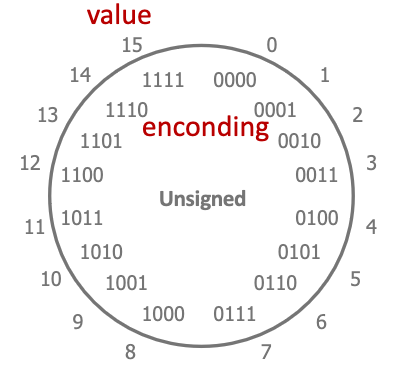
\includegraphics[scale=0.4]{img/unsigned_encoding.png}
        \caption{Unsigned encoding of 4-bit integers in C. } 
        \label{fig:unsigned_encoding}
      \end{figure}
    \end{theorem}

    \begin{example}[Bit Representation of Unsigned Integers in C]
      We can see for ourselves how these numbers are represented in bits. Printing the values out in binary requires to make new functions, but we can easily convert from hex to binary. 

      \noindent\begin{minipage}{.5\textwidth}
      \begin{lstlisting}[]{Code}
        int main() { 

          unsigned short x = 13; 
          unsigned int y = 256;

          printf("%x\n", x);
          printf("%x\n", y);

          return 0; 
        }
      \end{lstlisting}
      \end{minipage}
      \hfill
      \begin{minipage}{.49\textwidth}
      \begin{lstlisting}[]{Output}
        d
        100 
        .
        .
        .
        .
        .
        .
        .
        .
      \end{lstlisting}
      \end{minipage}
    \end{example}

    So far, the process of converting unsigned numbers to bits seemed simple. Now let's introduce signed integers. 

    \begin{definition}[Signed Integer Types in C]
      In C, there are several signed integer types. We use this hierarchical method to give flexibility to the programmer on the size of the integer and whether it is signed or not. 
      \begin{enumerate} 
        \item A \textbf{signed short} is 2 bytes long and can be represented as a 4-digit hex or 16 bits, with values in $[-32,768: 32,767]$. 
        \item A \textbf{signed int} is 4 bytes long and can be represented as an 8-digit hex or 32 bits, with values in $[-2,147,483,648: 2,147,483,647]$. 
        \item A \textbf{signed long} is 8 bytes and can be represented as an 16-digit hex or 64 bits, but they are only guaranteed to be stored in 32 bits in other systems. 
        \item A \textbf{signed long long} is 8 bytes and can be represented as an 16-digit hex or 64 bits, and they are guaranteed to be stored in 64 bits in other systems. 
      \end{enumerate}
    \end{definition}

    To store signed integers, it is intuitive to simply take the first (left-most) bit and have that be the sign. Therefore, we lose one significant figure but gain information about the sign. However, this has some problems: first, there are two representations of zeros: $-0$ and $+0$. Second, the continuity from $-1$ to $0$ is not natural. It is best explained through an example, which doesn't lose much insight into the general case. 

    \begin{example}[Problems with the Signed Magnitude]
      Say that you want to develop the signed magnitude representation for 4-bit integers in C. Then, you can imagine the following diagram to represent the numbers. 
      \begin{figure}[H]
        \centering 
        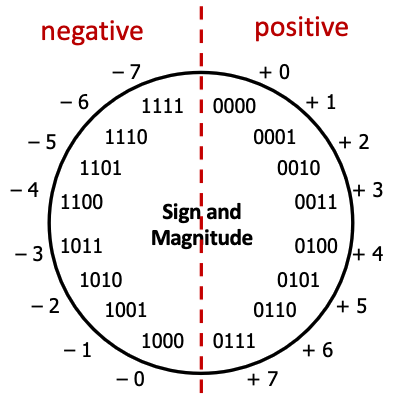
\includegraphics[scale=0.4]{img/signed_magnitude_encoding.png}
        \caption{Signed magnitude encoding of 4-bit integers in C.} 
        \label{fig:signed_magnitude_encoding}
      \end{figure}
      You can see that there are some problems: 
      \begin{enumerate}
        \item There are two representations for $0$, which is 0000 and 1000. 
        \item -1 (1001) plus 1 becomes -2 (1010). 
        \item The lowest number -7 (1111) plus 1 goes to 0 (0000) when it should go to -6 (1100). 
        \item The highest number 7 (0111) plus 1 goes to 0 (1000). 
      \end{enumerate}
    \end{example}

    An alternative way is to use the two's complement representation, which solves both problems and makes it more natural. 

    \begin{theorem}[Bit Representation of Signed Integers in C]
      The \textbf{two's complement} representation is a way to represent signed integers in binary. It is defined as follows. Given that you want to store a decimal number $p$ in $n$ bits, 

      \begin{enumerate}
        \item If $p$ is positive, then take the binary expansion of that number, which should be at most $n-1$ bits (no overflow), pad it with $0$s on the left. 
        \item If $p$ is negative, then you can do two things: First, take the binary expansion of the positive number, flip all the bits, and add 1. Or second, represent $p = q - 2^n$, take the binary representation of $q$ in $n-1$ bits, and add a $1$ to the left. 
      \end{enumerate}
      If you have a binary number $b = b_{n}b_{n-1}\cdots b_1$ then to convert it to a decimal number, you simply calculate 
      \begin{equation}
        q = -b_{n}2^{n-1} + b_{n-1}2^{n-2} + \cdots + b_1
      \end{equation}
      \begin{figure}[H]
        \centering 
        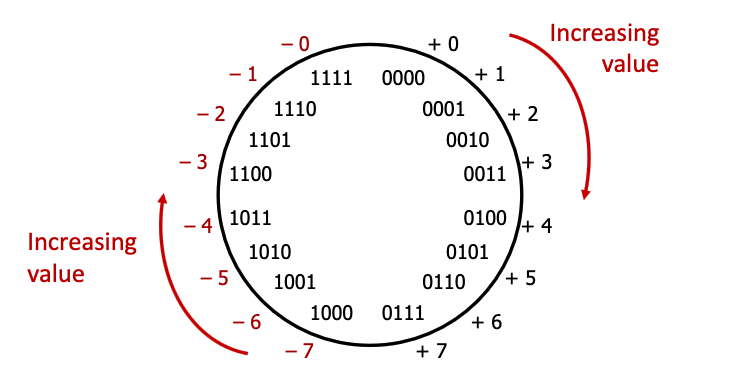
\includegraphics[scale=0.4]{img/twos_complement_encoding.png}
        \caption{Two's complement encoding of 4-bit integers in C.} 
        \label{fig:twos_complement_encoding}
      \end{figure}
    \end{theorem}

    \begin{example}[Bit Representation of Signed Integers in C]
      We can see for ourselves how these numbers are represented in bits. 

      \noindent\begin{minipage}{.5\textwidth}
      \begin{lstlisting}[]{Code}
        int main() { 

          short short_pos = 13; 
          short short_neg = -25; 
          int int_pos = 256;
          int int_neg = -512; 

          printf("%x\n", short_pos);
          printf("%x\n", short_neg);
          printf("%x\n", int_pos);
          printf("%x\n", int_neg);

          return 0; 
        }
      \end{lstlisting}
      \end{minipage}
      \hfill
      \begin{minipage}{.49\textwidth}
      \begin{lstlisting}[]{Output}
        d
        ffe7
        100
        ffffffe00
        .
        .
        .
        .
        .
        .
        .
        .
        .
        .
      \end{lstlisting}
      \end{minipage}
    \end{example}

    \begin{figure}[H]
      \centering 
      \noindent\begin{minipage}{.5\textwidth}
      \begin{lstlisting}[]{Code}
        #include<stdio.h>
        #include<stdbool.h>

        int main() {
          printf("%lu\n", sizeof(bool)); 
          printf("%lu\n", sizeof(short)); 
          printf("%lu\n", sizeof(int)); 
          printf("%lu\n", sizeof(long)); 
          printf("%lu\n", sizeof(long long)); 
          return 0; 
        }
      \end{lstlisting}
      \end{minipage}
      \hfill
      \begin{minipage}{.49\textwidth}
      \begin{lstlisting}[]{Output}
        1
        2
        4
        8
        8
        .
        .
        .
        .
        .
        .
      \end{lstlisting}
      \end{minipage}
      \caption{Size of various integer types in C with the \texttt{sizeof}.} 
      \label{fig:integer_size}
    \end{figure}


    \subsubsection{Arithmetic Operations on Binary Numbers}

      \begin{theorem}[Inversion of Binary Numbers]
        Given a binary number $p$, to compute $-p$, simply invert the bits and add 1.
      \end{theorem}

      \begin{theorem}[Addition and Subtraction of Binary Numbers]
        Given two binary numbers $p$ and $q$. 
        \begin{enumerate}
          \item To compute $p + q$, simply add the numbers together as you would in base 10, but carry over when the sum is greater than 1. 
          \item To compute $p - q$, you can invert $q$ to $-q$ and compute $p + (-q)$. 
        \end{enumerate}
      \end{theorem}

      % TODO: Bitshift and Bitwise Operations

  \subsection{Float Family} 

  \begin{definition}[Floating Point Types in C]
    In C, there are several floating point types. We use this hierarchical method to give flexibility to the programmer on the size of the integer and whether it is signed or not. 
    \begin{enumerate} 
      \item A \textbf{float} is 4 bytes long and can be represented as an 8-digit hex or 32 bits, with values in $[1.2 \times 10^{-38}: 3.4 \times 10^{38}]$. 
      \item A \textbf{double} is 8 bytes long and can be represented as an 16-digit hex or 64 bits, with values in $[2.3 \times 10^{-308}: 1.7 \times 10^{308}]$. 
      \item A \textbf{long double} is 8 bytes and can be represented as an 16-digit hex or 64 bits, but they are only guaranteed to be stored in 80 bits in other systems. 
    \end{enumerate}
  \end{definition}

  \begin{theorem}[Bit Representation of Floating Point Types in C]
    Floats are actually like signed magnitude. We have 
    \begin{equation} 
      (-1)^n \times 2^{e - 127} \times 1.s
    \end{equation}
    where 
    \begin{center} 
      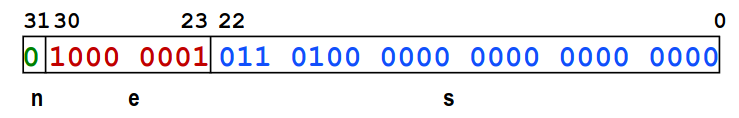
\includegraphics[scale=0.5]{img/float_encoding.png}
    \end{center}
    Doubles encode 64 bits, so not we have exponent having 11 bits (so bias is not 1023) and 52 bits for mantissa. 
  \end{theorem}

\section{Memory} 

  \begin{definition}[Memory]
    The \textbf{memory} is where the computer stores data and instructions, which can be though of as a giant array of memory addresses, with each containing a byte. This data consists of graphical things or even instructions to manipulate other data. It can be visualized  as a long array of boxes that each have an \textbf{address} (where it is located) and \textbf{contents} (what is stored in it).

    Memory simply works as a bunch of bits in your computer with each bit having some memory address, which is also a bit. For example, the memory address \texttt{0b0010} (2) may have the bit value of \texttt{0b1} (1) stored in it. 

    \begin{figure}[H]
      \centering 
      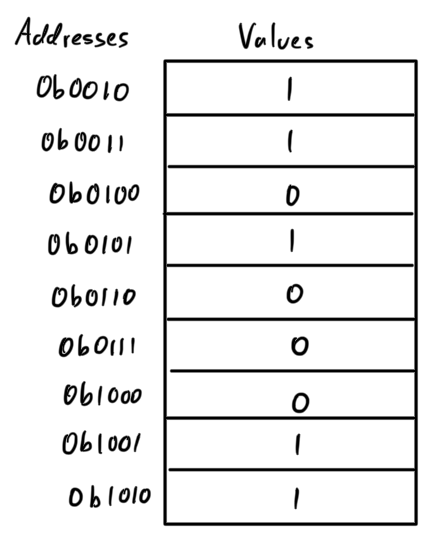
\includegraphics[scale=0.4]{img/memory_visual_bit.png}
      \caption{Visualization of memory as a long array of boxes of bits. }
      \label{fig:memory_visual_bit}
    \end{figure}

    However, computers do not need this fine grained level of control on the memory, and they really work at the Byte level rather than the bit level. Therefore, we can visualize the memory as a long array of boxes indexed by \textit{Bytes}, with each value being a byte as well. In short, the memory is \textbf{byte-addressable}. In certain arthitectures, some systems are \textbf{word-addressable}, meaning that the memory is addressed by words, which are 4 bytes.\footnote{Note that in here the size of a word is 2 bytes rather than 4 as stated above. This is just how it is defined in some \texttt{x86} architectures.}

    \begin{figure}[H]
      \centering 
      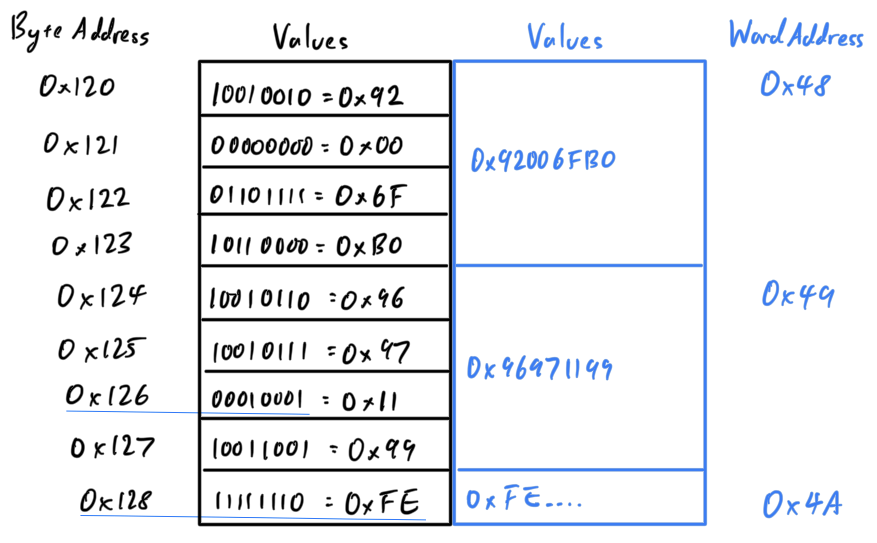
\includegraphics[scale=0.4]{img/memory_visual_byte.png}
      \caption{Visualization of memory as a long array of boxes of bytes. Every address is a byte and its corresponding value at that address is also a byte, though we represent it as a 2-digit hex. } 
      \label{fig:memory_visual_byte}
    \end{figure}
  \end{definition}

  In the examples above, I listed the memory addresses as a 3 hex character (1.5 bytes) for brevity. In reality, the number of bytes that a memory address takes is much longer. 

  \begin{definition}[32 and 64 Bit Machines]
    There are two types of machines that tend to format these boxes very differently: 32-bit and 64-bit machines. 
    \begin{enumerate}
      \item 32 bit machines store addresses in 32 bits, so they can have $2^{32}$ addresses, which is about 4 GB of memory. 
      \item 64 bit machines store addresses in 64 bits, so they can have $2^{64}$ addresses, which is about 16 EB of memory. This does not mean that the actual RAM is 16 EB, but it means that the machine can \textit{handle} that much memory. 
      \begin{lstlisting} 
        ...
        0x00007FFF7FBFF860 --> 0b000000000000000000000000011111111111
                               111101111111101111111111100001100000
        0x00007FFF7FBFF861 --> 0b000000000000000000000000011111111111
                               111101111111101111111111100001100001
        0x00007FFF7FBFF862 --> 0b000000000000000000000000011111111111
                               111101111111101111111111100001100010
        0x00007FFF7FBFF863 --> 0b000000000000000000000000011111111111
                               111101111111101111111111100001100011
        0x00007FFF7FBFF864 --> 0b000000000000000000000000011111111111
                               111101111111101111111111100001100100
        ...
      \end{lstlisting}
    \end{enumerate}
    The numbers typically mean the size of the type that the machine works best with, so all memory addresses will be 32 or 64 bits wide. Most machines are 64-bits, and so everything in this notes will assume that we are working with a 64 bit machine. As we will later see, this is why pointers are 8 bytes long, i.e. 64 bits. This is because the memory addresses are 64 bits long, though all of them are not used. 
  \end{definition}

  With this structure in mind and knowing the size of some primitive types, we can now focus on how declaring them works in the backend. 

  \begin{definition}[Declaration, Initialization]
    Assigning a value to a variable is a two step process, which is often not distinguished in high level languages like Python. 
    \begin{enumerate}
      \item You must first \textbf{initialize} the variable by setting aside the correct number of bytes in memory. 
      \item You must then \textbf{assign} that variable to be some actual value. 
    \end{enumerate}
    The two step process is often called declaration. 
  \end{definition}

  This is the reason why C is statically, or strongly, typed. In order to set aside some memory for a variable, you must know how big that variable will be, which you know by its type. This makes sense. We can first demonstrate how to both initialize and declare a variable. 

  \begin{figure}[H]
    \centering 
    \noindent\begin{minipage}{.5\textwidth}
    \begin{lstlisting}[]{Code}
      int main() {
        // declaring 
        int x = 4;   
        printf("%p\n", &x); 
        
        // initializing and assigning
        int y; 
        printf("%p\n", &y); 
        y = 3; 
        printf("%p\n", &y); 

        return 0; 
      }
    \end{lstlisting}
    \end{minipage}
    \hfill
    \begin{minipage}{.49\textwidth}
    \begin{lstlisting}[]{Output}
      0x16d37ee68
      0x16d37ee64
      0x16d37ee64 
      .
      .
      .
      .
      .
      .
      .
      .
      .
      .
    \end{lstlisting}
    \end{minipage}
    \caption{How to declare variables in C. As you can see, by initializing \texttt{y}, the memory address is already assigned and it doesn't change when you assign it. The address is only shown to be 9 hex digits long, but it is actually 16 hex digits long and simply 0 padded on the left. } 
    \label{fig:declaring_initializing_variables}
  \end{figure}

  One question that may come to mind is, what is the value of the variable if you just initialize it? After all the value at that address that is initialized must be either $0$s or $1$s. Let's find out. 

  \begin{figure}[H]
    \centering 
    \noindent\begin{minipage}{.5\textwidth}
    \begin{lstlisting}[]{Code}
      int main() { 
        int y; 
        printf("%d\n", y); 
        y = 3; 
        printf("%d\n", y); 

        return 0; 
      }
    \end{lstlisting}
    \end{minipage}
    \hfill
    \begin{minipage}{.49\textwidth}
    \begin{lstlisting}[]{Output}
      6298576 
      3
      .
      .
      .
      .
      .
      .
    \end{lstlisting}
    \end{minipage}
    \caption{The value of an uninitialized variable is some random number. } 
    \label{fig:uninitialized_variable}
  \end{figure}

  It may be interesting to see how this random unititialized value is generated. It is simply the value that was stored in that memory address before, and it is not cleared when you initialize it, so you should not use this as a unifom random number generator. 

  It is intuitive to think that given some multi-byte object like an \texttt{int} (4 bytes), the beginning of the int would be the lowest address and the end of the int would be the highest address, like how consecutive integers are stored in an array. However, this is not always the case (almost always not the case since most computers are little-endian).  

  \begin{definition}[Endian Architecture]
    Depending on the machine architecture, computers may store these types slightly differently in their \textit{byte} order. Say that we have an integer of value \texttt{0xA1B2C3D4} (4 bytes). Then, 
    \begin{enumerate} 
      \item A \textbf{big-endian architecture} (e.g. SPARC, z/Architecture) will store it so that the least significant byte has the highest address.
      \item A \textbf{little-endian architecture} (e.g. x86, x86-64, RISC-V) will store it so that the least significant byte has the lowest address. 
      \item A \textbf{bi-endian architecture} (e.g. ARM, PowerPC) can specify the endianness as big or little. 
    \end{enumerate}

    \begin{figure}[H]
      \centering 
      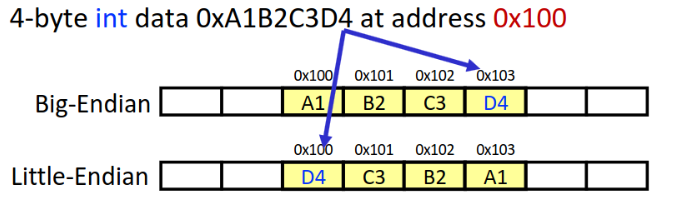
\includegraphics[scale=0.4]{img/endianness.png}
      \caption{The big vs little endian architectures. } 
      \label{fig:endianness}
    \end{figure}
  \end{definition}

  We can simply print out the hex values of primitive types to see how they are stored in memory, but it does not provide the level of details that we want on which bytes are stored where. At this point, we must use certain \textbf{debuggers} to directly look at the memory. For x86 architectures, we can use \texttt{gdb} and for ARM architectures, we can use \texttt{lldb}. At this point, we need to understand assembly to look through debuggers, so we will provide the example here. 

  \begin{example}[Endianness of C Int in x86]
    To do. 
  \end{example}

  \subsection{Type Casting}


  \subsection{Pointers}

    We have learned how to declare/initialize a variable, which frees up some space in the memory and possibly assigns a value to it. One great trait of C is that we can also store the memory address of a variable in another variable called a pointer. You access both the memory and the value at that memory with this pointer variable. 

    \begin{definition}[Pointer Variable]
      A \textbf{pointer} variable/type is a variable that stores the memory address of another variable. 
      \begin{enumerate}
        \item You can declare a pointer in the same way that you declare a variable, but you must add a asterisk in front of the variable name. 
        \item The size of this variable is the size of the memory address, which is 8 bytes in a 64-bit architecture. 
        \item To get the value of the variable that the pointer points to, called \textbf{dereferencing}, you simply put a asterisk in front of the pointer. This is similar to how you put a ampersand in front of a variable to get its memory address. 
      \end{enumerate}

      \begin{figure}[H]
        \centering 
        \noindent\begin{minipage}{.5\textwidth}
        \begin{lstlisting}[]{Code}
          int main() { 
            // declare an integer 
            int x = 4; 
            printf("x = %d\n", x); 
            printf("&x = %p\n", &x); 

            // declare pointer 
            int *p = &x; 
            printf("p = %p\n", p); 
            printf("*p = %d\n", *p); 

            // initialize pointer 
            int *q; 
            q = &x; 
            printf("q = %p\n", q); 
            printf("*q = %d\n", *q); 
            return 0; 
          }
          
        \end{lstlisting}
        \end{minipage}
        \hfill
        \begin{minipage}{.49\textwidth}
        \begin{lstlisting}[]{Output}
          x = 4
          &x = 0x16d49ae68
          p = 0x16d49ae68
          *p = 4
          q = 0x16d49ae68
          *q = 4
          .
          .
          .
          .
          .
          .
          .
          .
          .
          .
          .
          .
        \end{lstlisting}
        \end{minipage}
        \caption{} 
        \label{fig:pointer_variable}
      \end{figure}
    \end{definition}

    Since the size of addresses are predetermined by the architecture, it may not seem like we need to know the underlying data type of what it points to, so why do we need to write strongly type the underlying data type? Remember that to do pointer arithmetic, you need to know how large the underlying data type is so that you can know how many bytes to move when traversing down an array. 

    Just like for regular variables, you may be curious on the value of an unassigned pointer. Let's take a look. 

    \begin{example}[Uninitialized Pointers]
    \begin{figure}[H]
      \centering 
      \noindent\begin{minipage}{.5\textwidth}
      \begin{lstlisting}[]{Code}
        int main() { 
          int x = 4; 
          int *p; 
          printf("p = %p\n", p); 
          printf("*p = %x\n", *p); 

          return 0; 
        }
      \end{lstlisting}
      \end{minipage}
      \hfill
      \begin{minipage}{.49\textwidth}
      \begin{lstlisting}[]{Output}
        p = 0x10249ff20
        *p = d100c3ff
        .
        .
        .
        .
        .
        .
      \end{lstlisting}
      \end{minipage}
      \caption{The value of an uninitialized pointer is some random address and at a random address it would be some random byte. } 
      \label{fig:uninitialized_pointer}
    \end{figure}
    \end{example}

    This is clearly not good, especially since the program compiles correctly and runs without any errors. This kind of pointer that hasn't been initialized is called a wild pointer. 

    \begin{definition}[Wild Pointer]
      A \textbf{wild pointer} is a pointer that has not been initialized to a known value. 
    \end{definition}

    To fix this, we must always initialize a pointer to a known value. This may come at a disadvantage, since now we can't reap the benefits of initializing first and assigning later. A nice compromise is to initialize the pointer to a null pointer. 

    \begin{definition}[Null Pointer]
      A \textbf{null pointer} is a pointer that has been initialized to a known value, which is the address 0x0. You can set the type of the pointer and then initialize it to \texttt{NULL}. 
    \begin{figure}[H]
      \centering 
      \noindent\begin{minipage}{.5\textwidth}
      \begin{lstlisting}[]{Code}
        int main() { 
          int *p = NULL; 
          printf("p = %p\n", p); 
          
          // the code below gives seg fault
          /* printf("*p = %d\n", *p); */

          int x = 4; 
          p = &x; 
          printf("p = %p\n", p); 
          printf("*p = %d\n", *p);
          return 0; 
        }
      \end{lstlisting}
      \end{minipage}
      \hfill
      \begin{minipage}{.49\textwidth}
      \begin{lstlisting}[]{Output}
        p = 0x0
        p = 0x16da72e5c
        *p = 4
        .
        .
        .
        .
        .
        .
        .
        .
        .
        .
      \end{lstlisting}
      \end{minipage}
      \caption{Initializing a null pointer. It is a good practice to initialize a pointer to a null value. } 
      \label{fig:null_pointer}
    \end{figure}
    \end{definition}

    Therefore, the null pointer allows you to set the type of the underlying data type, but the actual address will be 0x0. You cannot dereference a null pointer, and doing so will give you a segmentation fault. There may be times when you do not even know the data type of the pointer, and for this you can use the void pointer, which now doesn't know the type of the variable that it points to but it does allocate address. 

    \begin{definition}[Void Pointer]
      A \textbf{void pointer} is a pointer that does not know the type of the variable that it points to. We can initialize it by simply setting the underlying type to be void. This initializes the address, which should always be 8 bytes, but trying to access the value of the variable is not possible. 
      \begin{figure}[H]
        \centering 
        \noindent\begin{minipage}{.5\textwidth}
        \begin{lstlisting}[]{Code}
          int main() { 
            void *p; 
            printf("p = %p\n", p); 
            int x = 4; 
            p = &x; 
            printf("%d", *((int*)p));
            return 0; 
          }
        \end{lstlisting}
        \end{minipage}
        \hfill
        \begin{minipage}{.49\textwidth}
        \begin{lstlisting}[]{Output}
          p = 0x102553f54
          4 
          .
          .
          .
          .
          .
          .
        \end{lstlisting}
        \end{minipage}
        \caption{Initialize a void pointer and then use typecasting to access the value of the variable that it points to. } 
        \label{fig:initialize_void_pointer}
      \end{figure}
    \end{definition}

  \subsection{Arrays and Pointer Arithmetic} 

    With pointers out of the way, we can talk about how arrays are stored in memory. 

    \begin{definition}[Array]
      A C array is a collection of elements of the same type, which are stored in contiguous memory locations. You can initialize and declare arrays in many ways, and access their elements with the index, e.g. \texttt{arr[i]}.
      \begin{enumerate}
        \item You declare an array of some constant number of elements $n$ with the elements themselves. 
          \begin{lstlisting} 
            int arr[5] = {1, 2, 3, 4, 5}; 
          \end{lstlisting}
        \item You declare an array with out its size $n$ and simply assign them. Then $n$ is automatically determined. 
          \begin{lstlisting} 
            int arr[] = {1, 2, 3, 4, 5}; 
          \end{lstlisting}
        \item You initialize an array of some constant size $c$, and then you assign each element of the array. 
          \begin{lstlisting} 
            int arr[5]; 
            for (int i = 0; i < 5; i++) {
              arr[i] = i + 1; 
            }
          \end{lstlisting}
      \end{enumerate}
      Unfortunately, C does not provide a built-in way to get the size of the array (like \texttt{len} in Python), so we must keep track of the size of the array ourselves. Furthermore, the address of the array is the address of where it begins at, i.e. the address of the first element. 
    \end{definition}

    You can literally see that the elements of the array are contiguous in memory by iterating through each element and printing out its address. 

    \begin{figure}[H]
      \centering 
      \noindent\begin{minipage}{.5\textwidth}
      \begin{lstlisting}[]{Code}
        int main(void) {
          // initialize array 
          int arr[5]; 
          for (int val = 1; val < 6; val++) {
            arr[val-1] = val * val;
          }

          int* p = &arr[0]; 
          for (int i = 0; i < 5; i++) {
            printf("Value at position %d : %d\n", i, arr[i]); 
            printf("Address at position %d : %p\n", i, p + i); 
          }

          return 0; 
        }        
      \end{lstlisting}
      \end{minipage}
      \hfill
      \begin{minipage}{.49\textwidth}
      \begin{lstlisting}[]{Output}
        Value at position 0 : 1
        Address at position 0 : 0x7ffd8636b0d0
        Value at position 1 : 4
        Address at position 1 : 0x7ffd8636b0d4
        Value at position 2 : 9
        Address at position 2 : 0x7ffd8636b0d8
        Value at position 3 : 16
        Address at position 3 : 0x7ffd8636b0dc
        Value at position 4 : 25
        Address at position 4 : 0x7ffd8636b0e0
        .
        .
        .
        .
        .
        .
        .
      \end{lstlisting}
      \end{minipage}
      \caption{Ints are 4 bytes long, so the address of the next element is 4 bytes away from the previous element, making this a contiguous array.} 
      \label{fig:contiguous_array}
    \end{figure}

    The most familiar implementation of an array is a string in C. 

    \begin{definition}[String]
      A string is an array of characters, which is terminated by a null character \texttt{\textbackslash 0}. You can initialize them in two ways: 
      \begin{enumerate}
        \item You can declare a string with the characters themselves, which you must make sure to end with the null character. 
          \begin{lstlisting} 
            char str[6] = {'H', 'e', 'l', 'l', 'o', '\0'}; 
          \end{lstlisting}
        \item You can declare them with double quotes, which automatically adds the null character. 
          \begin{lstlisting} 
            char str[] = "Hello"; 
          \end{lstlisting}
      \end{enumerate}
      Note that for whatever string we initialize, the size of the array is the number of characters plus 1. 
    \end{definition}

    To access elements of an array, you simply use the index of the element, e.g. \texttt{arr[i]}, but in the backend, this is implemented with \textit{pointer arithmetic}. 

    \begin{definition}[Pointer Arithmetic]
      Pointer arithmetic is the arithmetic of pointers, which is done by adding or subtracting an integer to a pointer. 
      \begin{enumerate}
        \item If you add an integer $n$ to a pointer $p$, e.g. \texttt{p + n}, then the new pointer will point to the $n$th element after the current element, with the next element being \texttt{sizeof(type)} bytes away from the pervious element. 
        \item If you subtract an integer $n$ from a pointer, then the pointer will point to the $n$th element before the current element. 
      \end{enumerate}
      This is why you can access the elements of an array with the index, since the index is simply the number of elements away from the first element.
    \end{definition}

    \begin{example}[Pointer Arithmetic with Arrays of Ints and Chars]
      Ints have a size of 4 bytes and chars 1 byte. You can see that using pointer arithmetic, the addresses of the elements of ints increment by 4 and those of the char array increment by 1. 
      \noindent\begin{minipage}{.5\textwidth}
      \begin{lstlisting}[]{Code}
        int main() { 
          int integers[3] = {1, 2, 3}; 
          char characters[3] = {'a', 'b', 'c'};
          int *p = &integers[0]; 
          char *q = &characters[0];
          
          printf("Array of Integers\n"); 
          for (int i = 0; i < 3; i++) { 
            printf("%p\n", integers+i); }

          printf("Array of Characters\n"); 
          for (int i = 0; i < 3; i++) { 
            printf("%p\n", characters+i); }
          return 0; 
        }
      \end{lstlisting}
      \end{minipage}
      \hfill
      \begin{minipage}{.49\textwidth}
      \begin{lstlisting}[]{Output}
        Array of Integers
        0x16d39ee58
        0x16d39ee5c
        0x16d39ee60
        .
        Array of Characters
        0x16d39ee50
        0x16d39ee51
        0x16d39ee52
        .
        .
        .
        .
        .
        .
      \end{lstlisting}
      \end{minipage}
    \end{example}

    Therefore, we can think of accessing the elements of an array as simply pointer arithmetic. 

    \begin{theorem}[Bracket Notation is Pointer Arithmetic]
      The bracket notation is simply pointer arithmetic in the backend. 
      \begin{figure}[H]
        \centering 
        \noindent\begin{minipage}{.5\textwidth}
        \begin{lstlisting}[]{Code}
          int main() { 
            int arr[3] = {1, 2, 3}; 
            int *p = &arr[0]; 

            for (int i = 0; i < 3; i++) { 
              printf("%d\n", arr[i]); 
              printf("%d\n", *(p+i)); 
            }
            return 0; 
          }
        \end{lstlisting}
        \end{minipage}
        \hfill
        \begin{minipage}{.49\textwidth}
        \begin{lstlisting}[]{Output}
          1
          1
          2
          2
          3
          3
          .
          .
          .
          .
        \end{lstlisting}
        \end{minipage}
        \caption{Accessing the elements of the list using both ways is indeed the same. } 
        \label{fig:bracket_pointer_arthimetic}
      \end{figure}
    \end{theorem}
   
  \subsection{Call by Value vs Call by Reference}
    When you call by reference, you are essentially modifying the value at a memory address, so it persists. 

  \subsection{Global, Stack, and Heap Memory}

    Everything in a program is stored in memory, variables, functions, and even the code itself. However, we will find out that they are stored in different parts of the memory. When a program runs, its application memory consists of four parts, as visualized in the Figure \ref{fig:memory_layout}. 
    \begin{enumerate} 
      \item The \textbf{code} is where the code text is stored. 
      \item The \textbf{global memory} is where all the global variables are stored. 
      \item The \textbf{stack} is where all of the functions and local variables are stored. 
      \item The \textbf{heap} is variable and can expand to as much as the RAM on the current system. We can specifically store whatever variables we want in the heap.
    \end{enumerate}

    We provide a visual of these four parts first, and we will go into them later. 
    \begin{figure}[H]
      \centering 
      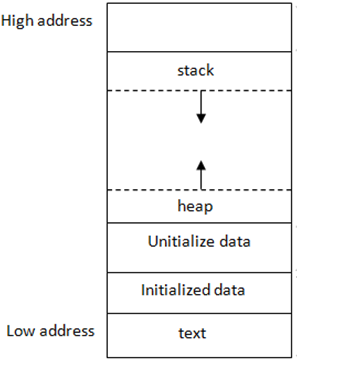
\includegraphics[scale=0.6]{img/memory_layout.png}
      \caption{The four parts of memory in a C program.} 
      \label{fig:memory_layout} 
    \end{figure}

    \begin{definition}[Code Memory]
      This is where the code text is stored. It is read-only and is not modifiable.
    \end{definition}

    In high level languages, we always talk about local and global scope. That is, variables defined within functions have a local scope in the sense that anything we modify in the local scope does not affect the global scope. We can now understand what this actually means by examining the backend.  The global scope variables are stored in the global memory, and all local variables (and functions) are stored in the stack. 


    \begin{definition}[Global Memory]
      This is where all the global variables are stored. 
    \end{definition}

    \begin{definition}[Stack Memory]
      This is where all of the functions and local variables are stored. As we will see later, the compiler will always run the main function, which must exist in your file. By the main function is a function itself, and therefore it has its own local scope. 

      Then, when you initialize any functions or local variables within those functions (which will be the majority of your code), all these will be stored in the stack, which is an literally an implementation of the stack data structure. It is LIFO, and the first thing that goes in is the \texttt{main} function and its local variables, which is referred to as the \textbf{stack frame}. You can't free memory in the stack unless its in the top of the stack. 
    \end{definition}

    To see what happens in the stack, we can go through an example. 

    \begin{example}[Going through the Stack]
      Say that you have the following code: 

      \begin{lstlisting} 
        int total; 
        int Square(int x) {
          return x*x; 
        }
        int SquareOfSum(int x, int y) {
          int z = Square(x + y); 
          return z; 
        }
        int main() { 
          int a = 4, b = 8;              
          total = SquareOfSum(a, b); 
          printf("output = %d", total); 
          return 0; 
        }
      \end{lstlisting}
      
      The memory allocation of this program will run as such: 
      \begin{enumerate} 
        \item The \texttt{total} variable is initialized and is put into global memory. 
        \item \texttt{main} is called. It is put into the stack. 
        \item The local variables \texttt{a=4} and \texttt{b=8} are initialized and are put into the stack. 
        \item The \texttt{SquareOfSum} function is called and put into the stack. 
        \item The input local variables \texttt{x=4}, \texttt{y=8}, \texttt{z} are initialized and put into the stack. 
        \item \texttt{x + y=12} is computed and put into the stack. 
        \item The \texttt{Square} function is called and put into the stack. 
        \item The \texttt{x=12} local variable of \texttt{Square} is initialized and put into the stack. 
        \item The CPU computes \texttt{x*x=144} and returns the output. The \texttt{Square} function is removed from the stack. 
        \item We assign \texttt{z=144} and \texttt{SquareOfSum} returns it. Now \texttt{SquareOfSum} is removed from the stack. 
        \item \texttt{total=144} is assigned in the global memory still. 
        \item The \texttt{printf} function is called and put into the stack. 
        \item The \texttt{printf} function prints the output and is removed from the stack. 
        \item The \texttt{main} function returns \texttt{0} and is removed from the stack, ending our application. 
      \end{enumerate}
    \end{example}


    One limitation of the stack is that its total available memory is fixed from the start, ranging from 1MB to 8MB, and so you can't initialize arrays of billions of integers in the stack. It will cause a memory overflow. In fact, the memory of the stack, along with the global and text memory, are assigned at compile time, making it a \textbf{static memory}. 

    Since the stack is really just a very small portion of available memory, the heap comes into rescue, which is the pool of memory available to you in RAM. 

    \begin{definition}[Heap Memory]
      The \textbf{heap memory} (nothing to do with the heap data structure) is a variable length (meaning it can grow at runtime) and \textbf{dynamically allocated} (meaning that we can assign memory addresses during runtime) memory that is limited to your computer's hardware. Unlike simply initializing variables to allocate memory as in the stack, we must use the \textbf{malloc} and \textbf{free} functions in C, and \textbf{new} and \textbf{delete} operations in C++. 
    \end{definition}

    \begin{definition}[malloc]
      
    \end{definition}

    \begin{definition}[free]
      
    \end{definition}

    The stack can store pointer variables that point to the memory address in the heap. So the only way to access variables in the heap is through pointer reference, and the stack provides you that window to access that big pool of heap memory. 


    One warning: if you allocate another address, the previous address does not get deallocated off the memory. 

    \begin{definition}[Memory Leak]
      
    \end{definition}

    On the other hand, if you free an address but have a pointer still pointing to that address, this is also a problem called the dangling pointer. 

    \begin{definition}[Dangling Pointer]
      
    \end{definition}

    At this point, we might be wondering why we need both a stack and a heap. Well the benefits of heaps are clearer since you can dynamically allocate memory, and you don't have the LIFO paradigm that is blocking you from deallocating memory that has been allocated in the beginning of your program. A problem with just having heap is that stacks can be orders of magnitude times faster when allocating/deallocating from it than the heap, and the sequence of function calls is naturally represented as a stack. 

  \subsection{Dynamic Memory Allocation}

    Let's talk about how \texttt{malloc} and \texttt{free} are implemented in C. If you make a for loop and simply print all the addresses that you allocate to. You will find that they can be quite random. After a program makes some calls to malloc and free, the heap memory can becomes fragmented, meaning that there are chunks of free heap space interspersed with chunks of allocated heap space. The heap memory manager typically keeps lists of different ranges of sizes of heap space to enable fast searching for a free extent of a particular size. In addition, it implements one or more policies for choosing among multiple free extents that could be used to satisfy a request.

    The free function may seem odd in that it only expects to receive the address of the heap space to free without needing the size of the heap space to free at that address. That’s because malloc not only allocates the requested memory bytes, but it also allocates a few additional bytes right before the allocated chunk to store a header structure. The header stores metadata about the allocated chunk of heap space, such as the size. As a result, a call to free only needs to pass the address of heap memory to free. The implementation of free can get the size of the memory to free from the header information that is in memory right before the address passed to free.


  \subsection{Structs}

\section{Central Processing Unit} 

    Now let's talk about how functions work on a deeper level. When we write a command, like \texttt{int x = 4}, we are manually looking for an address (in the stack, global, or heap) and rewriting the bits that are at that address. Functions are just an automated way to do this, and all these modifications and computations are done by the CPU. 

    \begin{definition}[Central Processing Unit]
      The CPU is responsible for taking instructions (data) from memory and executing them. 
      \begin{enumerate} 
        \item The CPU is composed of \textbf{registers} (different from the cache), which are small, fast storage locations. These registers can either be \textbf{general purpose} (can be used with most instructions) or \textbf{special purpose} (can be accessed through special instructions, or have special meanings/uses, or are simply faster when used in a specific way).
        \item The CPU also has an \textbf{arithmetic unit} and \textbf{logic unit}, which is responsible for performing arithmetic and logical operations. 
        \item The CPU also has a \textbf{control unit}, which is responsible for fetching instructions from memory through the \textbf{databus}, which is literally a wire connecting the CPU and RAM, and executing them. 
      \end{enumerate}
      It executes instructions from memory one at a time and executes them, known as the \textbf{fetch-execute cycle}. It consists of 4 main operations. 
      \begin{enumerate} 
        \item \textbf{Fetch}: The \textbf{program counter}, which holds the memory address of the next instruction to be executed, tells the control unit to fetch the instruction from memory through the databus. 
        \item \textbf{Decode}: The fetched data is passed to the \textbf{instruction decoder}, which figures out what the instruction is and what it does and stores them in the registers.
        \item \textbf{Execute}: The arithmetic and logic unit then carries out these operations. 
        \item \textbf{Store}: Then it puts the results back on the databus, and stores them back into memory.
      \end{enumerate} 
      The CPU's \textbf{clock cycle} is the time it takes for the CPU to execute one instruction. More specifically, the clock cycle refers to a single oscillation of the clock signal that synchronizes the operations of the processor and the memory (e.g. fetch, decode, execute, store), and decent computers have clock cycles of at least $2.60$GHz (2.6 billion clock cycles per second). 
    \end{definition}

    Therefore, in order to actually do computations on the data stored in the memory, the CPU must first fetch the data, perform the computations, and then store the results back into memory. This can be done in two ways.

    \begin{enumerate}
      \item Load and Store Operations: CPUs use load instructions to move data from memory to registers (where operations can be performed more quickly) and store instructions to move the modified data back into memory.
      \item If the data is too big to fit into the registers, the CPU will use the \textbf{cache} to store the data, and in worse cases, the actual memory itself. Compilers optimize code by maximizing the use of registers for operations to minimize slow memory access. This is why you often see assembly code doing a lot in registers.
    \end{enumerate}

    To clarify, let us compare registers and memory. Memory is addressed by an unsigned integer while registers have names like \texttt{\%rsi}. Memory is much bigger at several GB, while the total register space is much smaller at around 128 bytes (may differ depending on the architecture). The memory is much slower than registers, which is usually on a sub-nanosecond timescale. The memory is dynamic and can grow as needed while the registers are static and cannot grow.

    The specific structure/architecture of the CPU is determined by the instruction set architecture (ISA), which can be thought of as a subset of the general computer architecture. 

    \begin{definition}[Instruction Set Architecture]
      The \textbf{ISA} or just \textbf{architecture} of a CPU is a high level description of what it can do. Some differences are listed here: 
      \begin{enumerate} 
        \item What instructions it can execute. 
        \item The instruction length and decoding, along with its complexity. 
        \item The performance vs power efficiency. 
      \end{enumerate}
      ISAs can be classified into two types. 
      \begin{enumerate} 
        \item The \textbf{complex instruction set computer} (CISC) is characterized by a large set of complex instructions, which can execute a variety of low-level operations. This approach aims to reduce the number of instructions per program, attempting to achieve higher efficiency by performing more operations with fewer instructions.
        \item The \textbf{reduced instruction set computer} (RISC) emphasizes simplicity and efficiency with a smaller number of instructions that are generally simpler and more uniform in size and format. This approach facilitates faster instruction execution and easier pipelining, with the philosophy that simpler instructions can provide greater performance when optimized.
      \end{enumerate}
    \end{definition}

    Just like how memory addressing is different between 32 and 64 bit machines, CPUs also use these schemes. While 32-bit processors have $2^{32}$ possible addresses in their cache, it turns out that 64-bit processors have a 48-address space. This is because CPU manufacturers took a shortcut. They use an instruction set which allows a full 64-bit address space, but current CPUs just only use the last 48-bits. The alternative was wasting transistors on handling a bigger address space which wasn't going to be needed for many years (since 48-bits is about 256TB). Just a bit of history for you. Finally, just to briefly mention, the input/output device, as the name suggests, processes inputs and displays outputs, which is how you can see what the program does. 

    \begin{example}[x86 Architecture]
      The x86 architecture is a CISC architecture, which is the most common architecture for personal computers. Here are important properties: 
      \begin{enumerate} 
        \item It is a complex instruction set computer (CISC) architecture, which means that it has a large set of complex instructions\footnote{https://en.wikipedia.org/wiki/X86\_instruction\_listings}. 
        \item Byte-addressing is enabled and words are stored in little-endian format.
        \item In the x86\_64 architecture, registers are 8 bytes long (and 4 bytes in x86\_32) and there are 16 total general purpose registers, for a total of only 128 bytes (very small compared to many GB of memory). Other special purpose registers are also documented in the wikipedia page, but it is not fully documented. 
      \end{enumerate}
    \end{example}

    \begin{example}[ARM Archiecture]
      Mainly in phones, tablets, laptops. 
    \end{example}

    \begin{example}[MIPS Architecture]
      MIPS is a RISC architecture, which is used in embedded systems such as digital home and networking equipment. 
    \end{example}


    \begin{definition}[Input/Output Device]
      The input device can read/load/write/store data from the outside world. The output device, which has \textbf{direct memory address}, can display data to the outside world. 
    \end{definition}

    One final note to mention, there are many assembly languages out there and various syntaxes. 

    \begin{example}[Assembly Syntax]
      The two most popular syntaxes are AT\&T and Intel. 
      \begin{enumerate}
        \item \textbf{Intel Syntax}: Specifies memory operands without any special prefixes. Square brackets [] are used to denote memory addresses. For example, mov eax, [ebx] means move the contents of the memory location pointed to by ebx into eax.

        \item \textbf{AT\&T Syntax}: Memory operands are denoted with parentheses () and include the \% prefix for registers. An instruction moving data from a memory location into a register might look like movl (\%ebx), \%eax, with additional prefixes for immediate values and segment overrides.
      \end{enumerate}
    \end{example}

    \begin{example}[Assembly Languages]
      The various assembly languages are as follows: 
      \begin{enumerate}
        \item \textbf{x86 Assembly} : The assembly language for Intel and AMD processors using the x86 architecture. Both AT\&T and Intel syntax are available. Tools or environments often allow switching between the two, with AT\&T being the default in GNU tools like GDB.
        
        \item \textbf{ARM Assembly} : The assembly language for ARM processors. Has its own unique syntax, not categorized as AT\&T or Intel. ARM syntax is closely tied to its instruction set architecture and is distinct from the x86 conventions.
        
        \item \textbf{MIPS Assembly} : The assembly language for MIPS processors. MIPS uses its own assembly language syntax, which is neither AT\&T nor Intel. MIPS syntax is designed around the MIPS instruction set architecture.
        
        \item \textbf{PowerPC Assembly} : The assembly language for PowerPC processors. PowerPC has its own syntax style, tailored to its architecture and instruction set, distinct from the AT\&T and Intel syntax models.
        
        \item \textbf{6502 Assembly} : Used in many early microcomputers and gaming consoles. Utilizes a syntax unique to the 6502 processor, not following AT\&T or Intel conventions.
        
        \item \textbf{AVR Assembly} : The assembly language for Atmel's AVR microcontrollers. AVR assembly follows its own syntax style, designed specifically for AVR microcontrollers and not based on AT\&T or Intel syntax.
        
        \item \textbf{Z80 Assembly} : Associated with the Z80 microprocessor, used in numerous computing devices in the late 20th century. Z80 assembly language has its own syntax that does not adhere to AT\&T or Intel syntax guidelines.
      \end{enumerate}
    \end{example}

    The most common one is the x86\_64, which is the one that we will be focusing on, with the AT\%T syntax. 

  \subsection{Circuits} 

    Let's go over some common logic gates. 
    
    \begin{definition}[AND, NOT, OR]
      
    \end{definition}

    \begin{definition}[XOR, NAND, NOR]
      
    \end{definition}

    \begin{definition}[NAND]
      
    \end{definition}

  \subsection{Registers}

    To understand anything that the CPU does, we must understand assembly language. In here, everything is done within registers, and we can see how the CPU fetches, decodes, and executes instructions. So what exactly are these registers? 

    \begin{definition}[Register]
      A register is a small, fast storage location within the CPU. It is used to store data that is being used immediately, and is the only place where the CPU can perform operations, which is why it must move data from memory to registers before it can perform operations on it. Everything in a register is in binary, at most 8 bytes, or 64 bits. 
    \end{definition}

    The specific type of registers that are available to a CPU depends on the computer architecture, or more specifically, the ISA, but here is a list of common ones for the x86-64. We have \texttt{\%rax}, \texttt{\%rbx}, \texttt{\%rcx}, \texttt{\%rdx}, \texttt{\%rsi}, \texttt{\%rdi}, \texttt{\%rbp}, \texttt{\%rsp}, \texttt{\%r8}, \texttt{\%r9}, \texttt{\%r10}, \texttt{\%r11}, \texttt{\%r12}, \texttt{\%r13}, \texttt{\%r14}, \texttt{\%r15}. Therefore, the x86-64 Intel CPU has a total of 16 registers for storing 64 bit data. However, it is important to know which registers are used for what. 

    \begin{definition}[Parameter Registers]
      Compilers typically store the first six parameters of a function in registers 
      \begin{equation}
        \texttt{\%rdi}, \texttt{\%rsi}, \texttt{\%rdx}, \texttt{\%rcx}, \texttt{\%r8}, \texttt{\%r9}, 
      \end{equation}
      respectively. 
    \end{definition}

    \begin{definition}[Return Register]
      The return value of a function is stored in the 
      \begin{equation}
        \texttt{\%rax} 
      \end{equation}
      register.
    \end{definition}

    \begin{definition}[Stack and Frame Pointers]
      The \texttt{\%rsp} register is the \textbf{stack pointer}, which points to the top of the stack. The \texttt{\%rbp} register is the \textbf{frame pointer}, or \textbf{base pointer}, which points to the base of the current stack frame. In a typical function prologue, \textbf{\%rbp} is set to the current stack pointer (\textbf{\%rsp}) value, and then \texttt{\%rsp} is adjusted to allocate space for the local variables of the function. This establishes a fixed point of reference (\texttt{\%rbp}) for accessing those variables and parameters, even as the stack pointer (\texttt{\%rbp}) moves.
    \end{definition}

    \begin{definition}[Instruction Pointer]
      The \texttt{\%rip} register is the \textbf{instruction pointer}, which points to the next instruction to be executed. Unlike all the registers that we have shown so far, programs cannot write directly to \texttt{\%rip}. 
    \end{definition}


    \begin{definition}[Notation for Accessing Lower Bytes of Registers]
      Sometimes, we need a more fine grained control of these registers, and x86-64 provides a way to access the lower bits of the 64 bit registers. We can visualize them with the diagram below. 
      \begin{figure}[H]
        \centering 
        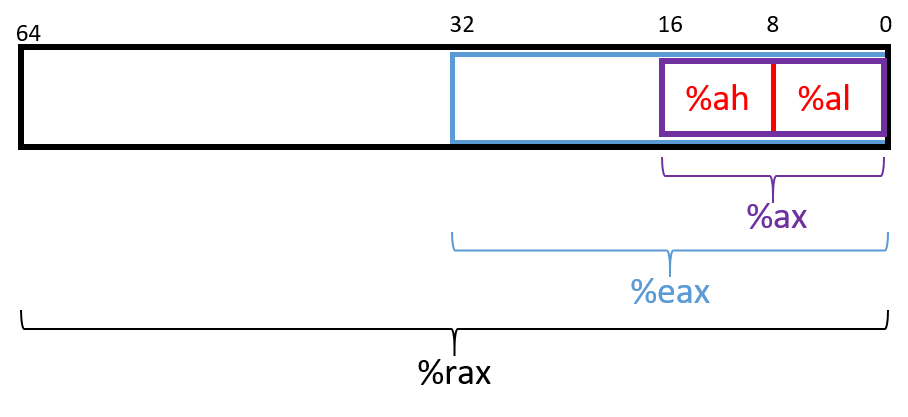
\includegraphics[scale=0.6]{img/register_subsets.png}
        \caption{The names that refer to subsets of register \texttt{\%rax}.} 
        \label{fig:register_subsets}
      \end{figure}
      A complete list is shown below. 
      \begin{table}[H]
        \centering
        \begin{tabular}{|l|l|l|l|}
        \hline
        \textbf{64-bit Register} & \textbf{32-bit Register} & \textbf{Lower 16 Bits} & \textbf{Lower 8 Bits} \\ \hline
        \%rax & \%eax & \%ax & \%al \\ \hline
        \%rbx & \%ebx & \%bx & \%bl \\ \hline
        \%rcx & \%ecx & \%cx & \%cl \\ \hline
        \%rdx & \%edx & \%dx & \%dl \\ \hline
        \%rdi & \%edi & \%di & \%dil \\ \hline
        \%rsi & \%esi & \%si & \%sil \\ \hline
        \%rsp & \%esp & \%sp & \%spl \\ \hline
        \%rbp & \%ebp & \%bp & \%bpl \\ \hline
        \%r8 & \%r8d & \%r8w & \%r8b \\ \hline
        \%r9 & \%r9d & \%r9w & \%r9b \\ \hline
        \%r10 & \%r10d & \%r10w & \%r10b \\ \hline
        \%r11 & \%r11d & \%r11w & \%r11b \\ \hline
        \%r12 & \%r12d & \%r12w & \%r12b \\ \hline
        \%r13 & \%r13d & \%r13w & \%r13b \\ \hline
        \%r14 & \%r14d & \%r14w & \%r14b \\ \hline
        \%r15 & \%r15d & \%r15w & \%r15b \\ \hline
        \end{tabular}
        \caption{Register mapping in x86-64 architecture}
        \label{table:register_mapping}
      \end{table}
    \end{definition}

  \subsection{Addressing Modes}

    Registers being 8 bytes mean that we can store memory addresses, and if we can store memory addresses, we can access memory, i.e. the values at those memory addresses. There are 4 ways to do this, called \textbf{addressing modes}: immediate, normal, displacement, and indexed. When we parse an instruction, its operands are either 
    \begin{enumerate}
      \item Constant (literal) values 
      \item Registers 
      \item Memory forms
    \end{enumerate}

    \begin{definition}[Immediate Addressing]
      Immediate addressing is when the operand is a constant value, used with a \$ sign. 
      \begin{equation}
        \texttt{\$val}
      \end{equation}
    \end{definition}

    \begin{example}[Immediate Addressing]
      \begin{lstlisting} 
        movq $0x4, %rax
      \end{lstlisting}
    \end{example}

    \begin{definition}[Normal Addressing]
      Normal addressing is when the operand is a register, used with a \% sign and the following syntax. The parentheses are used to dereference the memory address like dereferencing a pointer in C. 
      \begin{equation}
        \texttt{(R) = Mem[Reg[R]]}
      \end{equation}
      where \texttt{R} is the register name, \texttt{Reg[R]} is the value in the register, and \texttt{Mem[Reg[R]]} is the value in the memory address pointed to by the register. 
    \end{definition}

    \begin{example}[Normal Addressing]
      The following example shows the source operand being a memory address, with normal addressing, and the destination operand being a register.  
      \begin{lstlisting} 
        movq (%rax), %rbx
      \end{lstlisting}
    \end{example}

    \begin{definition}[Displacement Addressing]
      When we have a memory address stored in a register, we can add an offset to it to access a different memory address. 
      \begin{equation}
        \texttt{D(R) = Mem[Reg[R] + D]}
      \end{equation}
      where \texttt{R} is the register name and \texttt{D} is a constant displacement that specifies offset. 
    \end{definition}

    \begin{example}[Displacement Addressing]
      The following example shows the source operand being a memory address and the destination operand being a register. They are both addressed normally. 
      \begin{lstlisting} 
        movq 8(%rdi), %rdx
      \end{lstlisting}
    \end{example}

    \begin{definition}[Indexed Addressing]
      Indexed addressing gives us more flexibility, allowing us to multiply the value in the register by a constant and add it to the value in another register. The general formula is shown as the top, but there are special cases: 
      \begin{align*}
        \texttt{D(Rb, Ri, S)} && = \texttt{Mem[Reg[Rb] + S*Reg[Ri] + D]} \\ 
        \texttt{D(Rb, Ri)} && = \texttt{Mem[Reg[Rb] + Reg[Ri] + D]} \\
        \texttt{(Rb, Ri, S)} && = \texttt{Mem[Reg[Rb] + S*Reg[Ri]]} \\ 
        \texttt{(Rb, Ri)} && = \texttt{Mem[Reg[Rb] + Reg[Ri]]} \\
        \texttt{(, Ri, S)} && = \texttt{Mem[S*Reg[Ri]]} 
      \end{align*}
      where \texttt{D} is a constant displacement of 1, 2, or 4 bytes, \texttt{Rb} is the base register (can be any of 8 integer registers), \texttt{Ri} is the index register (can be any register except \texttt{rsp}), and \texttt{S} is the scale factor (1, 2, 4, or 8).
      
    \end{definition}

    \begin{example}[Indexed Addressing]
      The following shows the source operand being a memory address and the destination operand being a register. Say that \texttt{\%rdx = 0xf000} and \texttt{\%rcx = 0x0100}. Then 
      \begin{equation}
        \texttt{0x80(,\%rdx,2) = Mem[2*0xF000 + 0x80] = Mem[0x1E080]}
      \end{equation}

      We see that 
      \begin{lstlisting} 
        movq 0x100(%rdi, %rsi, 8), %rdx
      \end{lstlisting}
    \end{example}

  \subsection{Instructions} 

      Now that we've gotten a sense of what these registers are and some commonalities between them, let's do some operations on them with instructions. 

      \begin{definition}[Instruction]
        An instruction is a single line of assembly code. It consists of some instruction followed by its (one or more) operands. The instruction is a mnemonic for a machine language operation (e.g. \texttt{mov}, \texttt{add}, \texttt{sub}, \texttt{jmp}, etc.). The \textbf{size specifier} can be appended to this instruction mnemonic to specify the size of the operands. 
        \begin{enumerate} 
          \item \textbf{b} (byte) for 1 byte 
          \item \textbf{w} (word) for 2 bytes
          \item \textbf{l} (long) for 4 bytes 
          \item \textbf{q} (quad word) for 8 bytes
        \end{enumerate}
        Note that due to backwards compatibility, word means 2 bytes in instruction names. Furthermore, the maximum size is 8 bytes since that is the size of each register in x86\_64. An operand can be of 3 types, determined by their \textbf{mode of access}:
        \begin{enumerate} 
          \item \textbf{Immediate addressing} is denoted with a \texttt{\$} sign, e.g. a constant integer data \texttt{\$1}. 
          \item \textbf{Register addressing} is denoted with a \texttt{\%} sign with the following register name, e.g. \texttt{\%rax}.
          \item \textbf{Memory addressing} is denoted with the hexadecimal address in memory, e.g. \texttt{0x034AB}.
        \end{enumerate}
      \end{definition}

      Like higher level programming languages, we can perform operations, do comparisons, and jump to different parts of the code. Instructions can be generally categorized into three types: 
      \begin{enumerate} 
        \item \textbf{Data Movement}: These instructions move data between memory and registers or between the registery and registery. Memory to memory transfer cannot be done with a single instruction. 
          \begin{lstlisting} 
            %reg = Mem[address]     # load data from memory into register
            Mem[address] = %reg     # store register data into memory
          \end{lstlisting}
        \item \textbf{Arithmetic Operation}: Perform arithmetic operation on register or memory data. 
          \begin{lstlisting} 
            %reg = %reg + Mem[address]     # add memory data to register
            %reg = %reg - Mem[address]     # subtract memory data from register
            %reg = %reg * Mem[address]     # multiply memory data to register
            %reg = %reg / Mem[address]     # divide memory data from register
          \end{lstlisting}
        \item \textbf{Control Flow}: What instruction to execute next both unconditional and conditional (if statements) ones. With if statements, loops can then be defined. 
          \begin{lstlisting} 
            jmp label     # jump to label
            je label      # jump to label if equal
            jne label     # jump to label if not equal
            jg label      # jump to label if greater
            jl label      # jump to label if less
            call label    # call a function
            ret           # return from a function
          \end{lstlisting}
      \end{enumerate}

      Now unlike compiled languages, which are translated into machine code by a compiler, assembly code is translated into machine code through a two-step process. First, we \textbf{assemble} the assembly code into an \textbf{object file} by an \textbf{assembler}, and then we \textbf{link} the object file into an executable by a \textbf{linker}. Some common assemblers are \textbf{NASM} (Netwide Assembler) and \textbf{GAS/AS} (GNU Assembler), and common linkers are \textbf{ld} (GNU Linker) and \textbf{lld} (LLVM Linker), both installable with \textbf{sudo pacman -S nasm ld}. 

    \subsubsection{Moving Instructions}

      \begin{definition}[mov]
        Let's talk about the \texttt{mov} instruction which copies data from the source to the destination (the data in the source still remains!) and has the syntax 
        \begin{equation}
          \texttt{mov\_ src, dest}
        \end{equation}
        \begin{enumerate}
          \item The source can be a register (\texttt{\%rsi}), a value (\texttt{\$0x4}), or a memory address (\texttt{0x4}).
          \item The destination can be a register or a memory address. 
          \item The \texttt{\_} is defined to be one of the size operands, which determine how big the data is. For example, we can call \texttt{movq} to move 8 bytes of data (which turns about to be the maximum size of a register). 
        \end{enumerate}
        A good diagram to see is the following: 
        \begin{center}  
          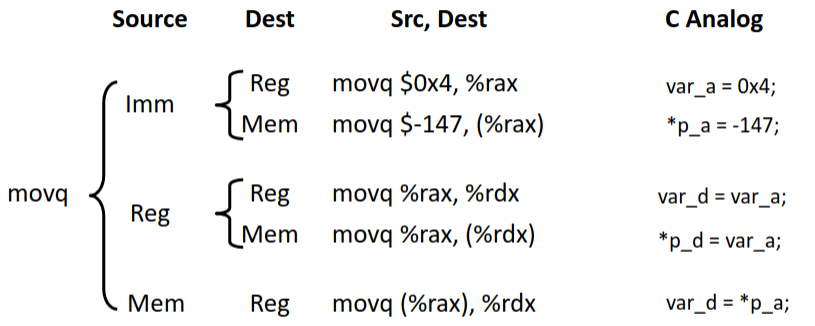
\includegraphics[scale=0.5]{img/movq.png}
        \end{center} 
      \end{definition}

      Even with just the mov instruction, we can look at a practical implementation of a C program in Assembly. 

      \begin{example}[Swap Function]
        Let us take a look at a function that swaps two integers. Let's see what they do. 
        \begin{enumerate}
          \item In C, we dereference both \texttt{xp} and \texttt{yp} (note that they are pointers to longs, so they store 8 bytes), and assign these two values to two temporary variables. Then, we assign the value of \texttt{yp} to \texttt{xp} and the value of \texttt{xp} to \texttt{yp}.
          \item In Assembly, we first take the registers \texttt{\%rdi} and \texttt{\%rsi}, which are the 1st and 2nd arguments of the function, dereference them with the parantheses, and store them in the temporary registers \texttt{\%rax} and \texttt{\%rdx}. Then, we store the value of \texttt{\%rdx} into the memory address of \texttt{\%rdi} and the value of \texttt{\%rax} into the memory address of \texttt{\%rsi}. Note that the input values (the actual of )
        \end{enumerate}

        \noindent\begin{minipage}{.5\textwidth}
        \begin{lstlisting}[]{Code}
          void swap(long *xp, long *yp) {
            long t0 = *xp;
            long t1 = *yp;
            *xp = t1;
            *yp = t0;
          }
        \end{lstlisting}
        \end{minipage}
        \hfill
        \begin{minipage}{.49\textwidth}
        \begin{lstlisting}[]{Output}
          swap:
            movq (%rdi), %rax
            movq (%rsi), %rdx
            movq %rdx, (%rdi)
            movq %rax, (%rsi)
            ret
        \end{lstlisting}
        \end{minipage}
      \end{example}

      \begin{definition}[movz and movs]
        The \texttt{movz} and \texttt{movs} instructions are used to move data from the source to the destination, but with zero and sign extension, respectively. It is used to copy from a smaller source value to a larger destination, with the syntax 
        \begin{align*}
          \texttt{movz\_\_ src, dest} \\ 
          \texttt{movs\_\_ src, dest} 
        \end{align*}
        where the first $\_$ is the size of the source and the second $\_$ is the size of the destination. 
        \begin{enumerate}
          \item The source can be from a memory or register. 
          \item The destination must be a register. 
        \end{enumerate}
      \end{definition}

      \begin{example}[Simple example with movz]
        Take a look at the code below. 
        \begin{lstlisting}
          movzbq %al, %rbx
        \end{lstlisting}
        The \texttt{\%al} represents the last byte of the \texttt{\%rax} register. It is 1 byte long. The \texttt{\%rbx} register is 8 bytes long, so we can fill in the rest of the 7 bytes with zeros. 
        \begin{center}  
          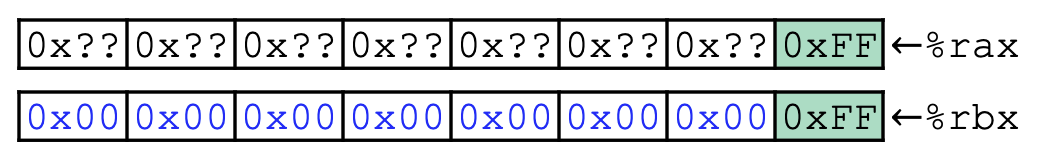
\includegraphics[scale=0.5]{img/movzbq.png}
        \end{center}
      \end{example}

      \begin{example}[Harder example with movs]
        Take a look at the code below. 
        \begin{lstlisting}
          movsbl (%rax), %ebx
        \end{lstlisting}
        You want to move the value at the memory address in \texttt{\%rax} into \texttt{\%ebx}. Since the source size is set to 1 byte, you take that byte, say it is \texttt{0x80}, from the memory, and then sign extend it (by a size of 4 bytes!) into \texttt{\%ebx}. Note that therefore, the first four bytes of \texttt{\%rbx} will not be affected since it's not a part of \texttt{\%ebx}. An exception to this is that in x86-64, any instruction that generates a 32-bit long word value for a register also sets the high-order 32 bits of the register to 0, so this ends up clearing the first 4 bytes to 0. 
        \begin{center}  
          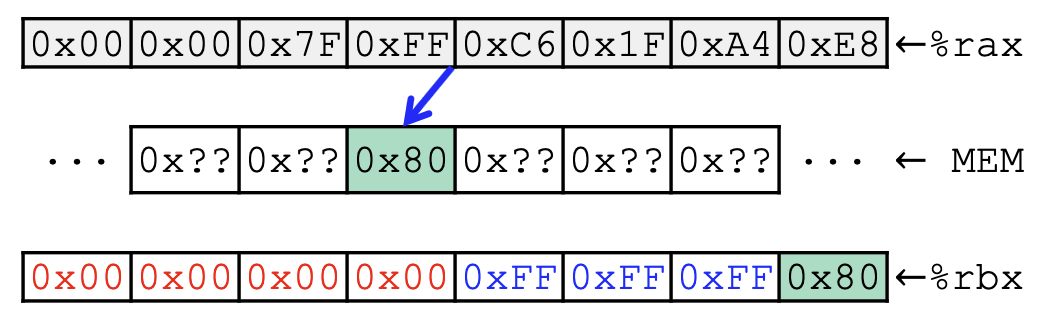
\includegraphics[scale=0.5]{img/movsbl.png}
        \end{center}
      \end{example}

    \subsubsection{Control Transfer on Stack}

      Say that you have the following C and Assembly code. 
      
      \begin{figure}[H]
        \centering 
        \noindent\begin{minipage}{.5\textwidth}
        \begin{lstlisting}[]{Code}
          int add(int x) {
            return x + 2; 
          }

          int main() {
            int a = 2; 
            int b = add(a); 
            return 0; 
          }
        \end{lstlisting}
        \end{minipage}
        \hfill
        \begin{minipage}{.49\textwidth}
        \begin{lstlisting}[]{Output}
          add: 
            movq %rdi, %rax 
            addq $2, %rax 
            ret 
          main:
            movq $3, $rdi 
            call add 
            movq $0, %rax 
            ret 
        \end{lstlisting}
        \end{minipage}
        \caption{A simple function. } 
        \label{fig:stack_example}
      \end{figure}

      If you go through the instructions, you see that in main, you first move \texttt{\$3} into the \texttt{\%rdi} register. Then, you call the \texttt{add} function, and within it you also have the \texttt{\%rdi} register. This is a conflict in the register, and we don't want to simply overwrite the value of \texttt{\%rdi} in the \texttt{main} function. Simply putting it to another register isn't a great idea since we can't always guarantee that it will be free. Therefore, we must use the memory itself. 

      Recall the stack, which we can think of as a giant array in which data gets pushed and popped in a last-in-first-out manner. The stack is used to store data and return addresses, and is used to manage function calls. Visually, we want to think of the elements getting pushed in from the bottom (upside down) towards lower memory addresses. 

      \begin{definition}[Stack Pointer]
        Note that every time we want to push or pop something from the stack, we must know \textit{where} to push or pop it. This is where the \textbf{stack pointer} comes in. It is a special register that always points to the top of the stack, and is used to keep track of the stack.
      \end{definition}

      \begin{definition}[Push and Pop]
        The \texttt{push} and \texttt{pop} instructions are used to push and pop data onto and off the stack, respectively. 
        \begin{align*}
          \texttt{push\_ src} && \texttt{rsp = rsp - 8; Mem[rsp] = src} \\
          \texttt{pop\_ dest} && \texttt{dest = Mem[rsp]; rsp = rsp + 8} 
        \end{align*}
        \begin{enumerate}
          \item When we push the source, we fetch the value at the source and store it at the memory address pointed to by the stack pointer \texttt{\%rsp}. Then, we decrement \texttt{\%rsp} by 8.
          \item When we pop from the stack, we fetch the value at the memory address pointed to by the stack pointer \texttt{\%rsp} and store it in the destination. Then, we increment \texttt{\%rsp} by 8.
        \end{enumerate}
        Note that no matter what the size of the operand, we always subtract 8 from the stack pointer. This is because the stack grows downwards, and we want to make sure that the next element is pushed into the next available space.
      \end{definition}

      Note that the register \texttt{\%rsp} is the stack pointer, which points to the top of the stack. The stack is used to store data and return addresses, and is used to manage function calls. 

      \begin{definition}[Push and Pop]
        The \texttt{push} and \texttt{pop} instructions are used to push and pop data onto and off the stack, respectively. 
        \begin{align*}
          \texttt{push\_ src} && \texttt{rsp = rsp - 8; Mem[rsp] = src} \\
          \texttt{pop\_ dest} && \texttt{dest = Mem[rsp]; rsp = rsp + 8} 
        \end{align*}
        The \texttt{\_} is a size operand, which determines how big the data is.
      \end{definition}

      \begin{definition}[Call and Ret]
        The \texttt{call} instruction pushes the return address onto the stack and jumps to the function. The \texttt{ret} instruction pops the return address from the stack and jumps to it.
      \end{definition}

      We also talked about how there is instruction code that is even below the stack that is stored. This is where all the machine code/assembly is stored, and we want to find out where we are currently at in this code. This is done with the program counter. 

      \begin{definition}[Program Counter, Instruction Pointer] 
        The \textbf{program counter}, or \textbf{instruction pointer}, is a special register \textbf{rip} that points to the current instruction in the program. It is used to keep track of the next instruction to be executed.
      \end{definition}

      Let's go through one long example to see in detail how this is calculated. 
      
      \begin{example}[Evaluating a Function]
        Say that we have the following C code. 
        \begin{lstlisting}
          int adder2(int a) {
            return a + 2; 
          }

          int main() {
            int x = 40; 
            x = adder2(x); 
            printf("x is: %d\n", x);
            return 0; 
          }
        \end{lstlisting}
        When we compile this program, we can view its full assembly code by calling \texttt{objdump -d a.out}. The output is quite long, so we will focus on the instruction for the \texttt{adder2} function. 
        \begin{figure}[H]
          \centering 
          \begin{lstlisting}
            0000000000400526 <adder2>:
            400526:       55                      push   %rbp
            400527:       48 89 e5                mov    %rsp,%rbp
            40052a:       89 7d fc                mov    %edi,-0x4(%rbp)
            40052d:       8b 45 fc                mov    -0x4(%rbp),%eax
            400530:       83 c0 02                add    $0x2,%eax
            400533:       5d                      pop    %rbp
            400534:       c3                      retq
          \end{lstlisting}
          \caption{The output of objdump for the \texttt{adder2} function. The leftmost column represents the addresses (in hex) of where the actual instructions lie. The second column represents the machine code that is being executed. The third column represents the assembly code.}
          \label{fig:adder2} 
        \end{figure}
        Note some things. Since \texttt{adder2} is taking in an integer input value, we want to load it into the lower 32 bits (4 bytes) of the \texttt{\%rdi} register, which is the first parameter. So we use \texttt{\%edi}. Likewise for the return value, we want to output an int so we use \texttt{\%eax} rather than \texttt{\%rax}. Let's go through some of the steps. 
        \begin{enumerate}
          \item By the time we get into calling \texttt{adder2}, we can take a look at the relevant registers. 

            \begin{center}
              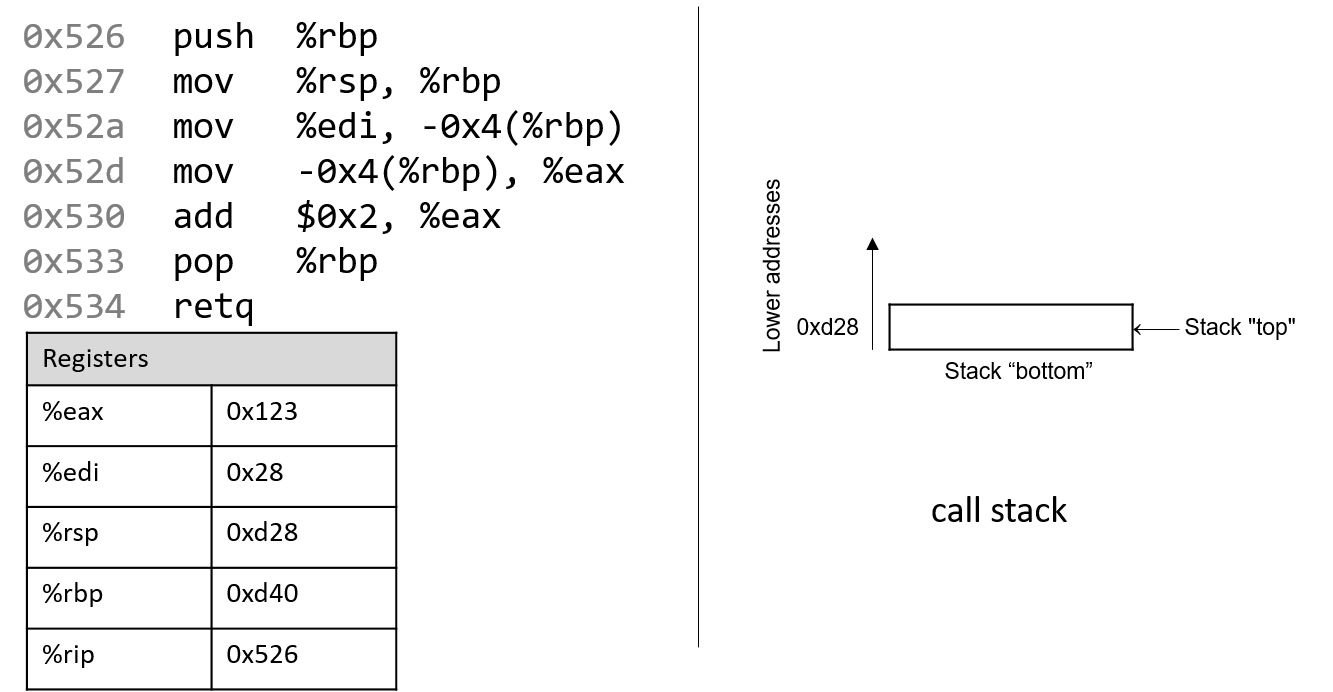
\includegraphics[scale=0.5]{img/ex1_1.png}
            \end{center}
            \begin{enumerate}
              \item First, the \texttt{\%eax} is filled with garbage, which are leftovers from previous programs that haven't been overwritten yet. 
              \item Second, the \texttt{\%edi=0x28} since we have set \texttt{x=40} in \texttt{main}, before calling \texttt{adder2}, so it lingers on. 
              \item \texttt{\%rsp=0xd28} since that is where the top of the stack is. 
              \item \texttt{\%rbp=0xd40} 
              \item \texttt{\%rip=0x526} since that is where we are currently at in our instruction (we are about to do it, but haven't done it yet). 
            \end{enumerate}

          \item When we execute the first line of code, we simply push the value at \texttt{\%rbp} into the stack. The top of the stack gets decremeneted by 8 and the value at \texttt{\%rbp} is stored there. This means that the top of the stack is at \texttt{\%rsp=0xd20} and the next instruction will be at \texttt{\%rip=0x527}.  

            \begin{center}
              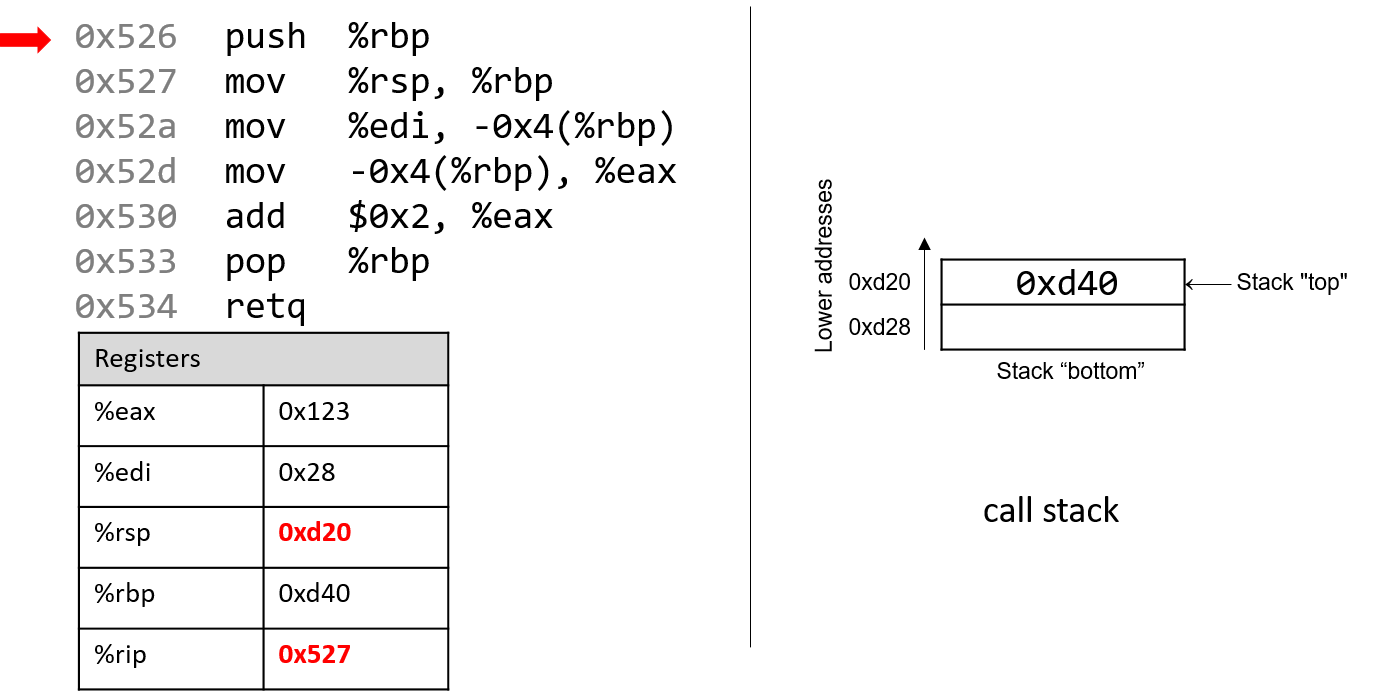
\includegraphics[scale=0.5]{img/ex1_2.png}
            \end{center}

          \item The reason we have pushed \texttt{\%rbp} onto the stack is that we want to save it before it gets overwritten by this next execution. We basically move the value of \texttt{\%rsp} into \texttt{\%rbp}, and the \texttt{\%rip} advances to the next instruction. \texttt{\%rip} moves to the next instruction. 

            \begin{center}
              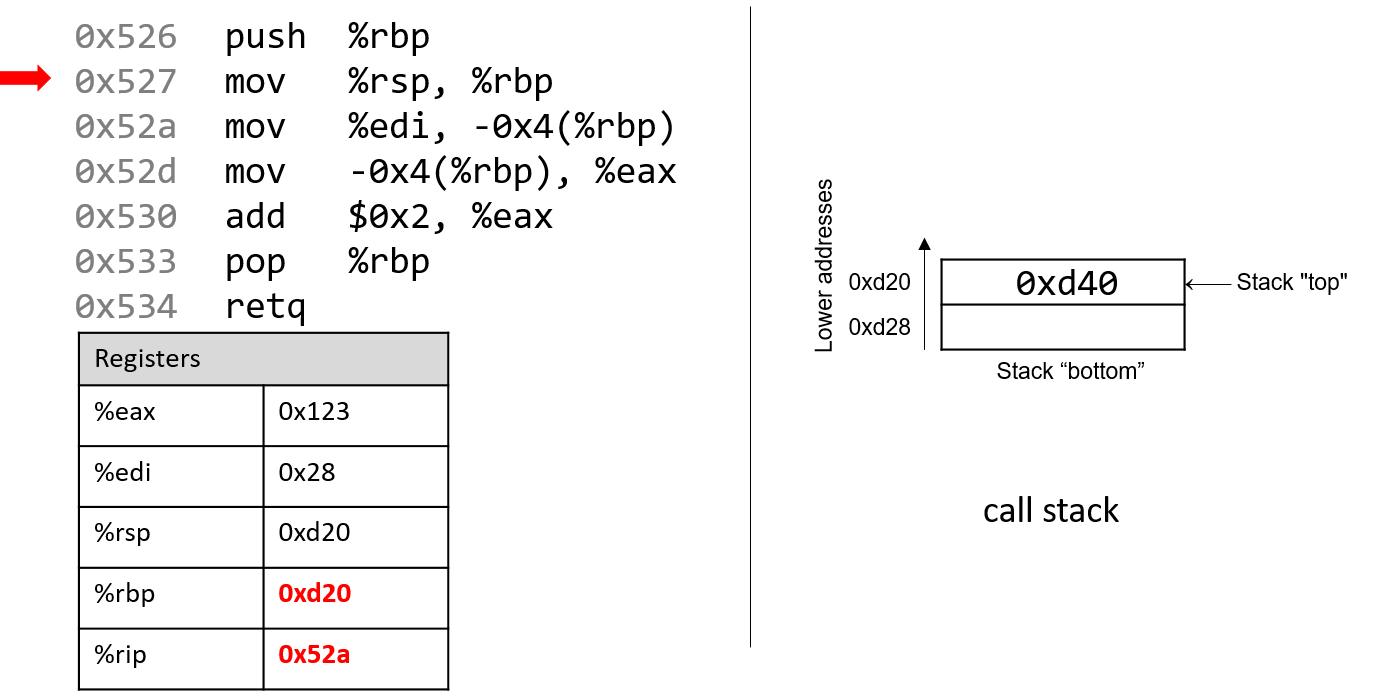
\includegraphics[scale=0.5]{img/ex1_3.png}
            \end{center}

          \item Now we want to take our first argument \texttt{\%edi} and store it in memory. Note that since this is 4 bytes, we can move this value into memory that is 4 bytes below the stack (\texttt{-0x4(\%rbp)}). Note that the storing the value of \texttt{\%edi} into memory doesn't affect the stack pointer \texttt{\%rsp}. As far as the program is concerned, the top of this stack is still address \texttt{0xd20}. 

            \begin{center}
              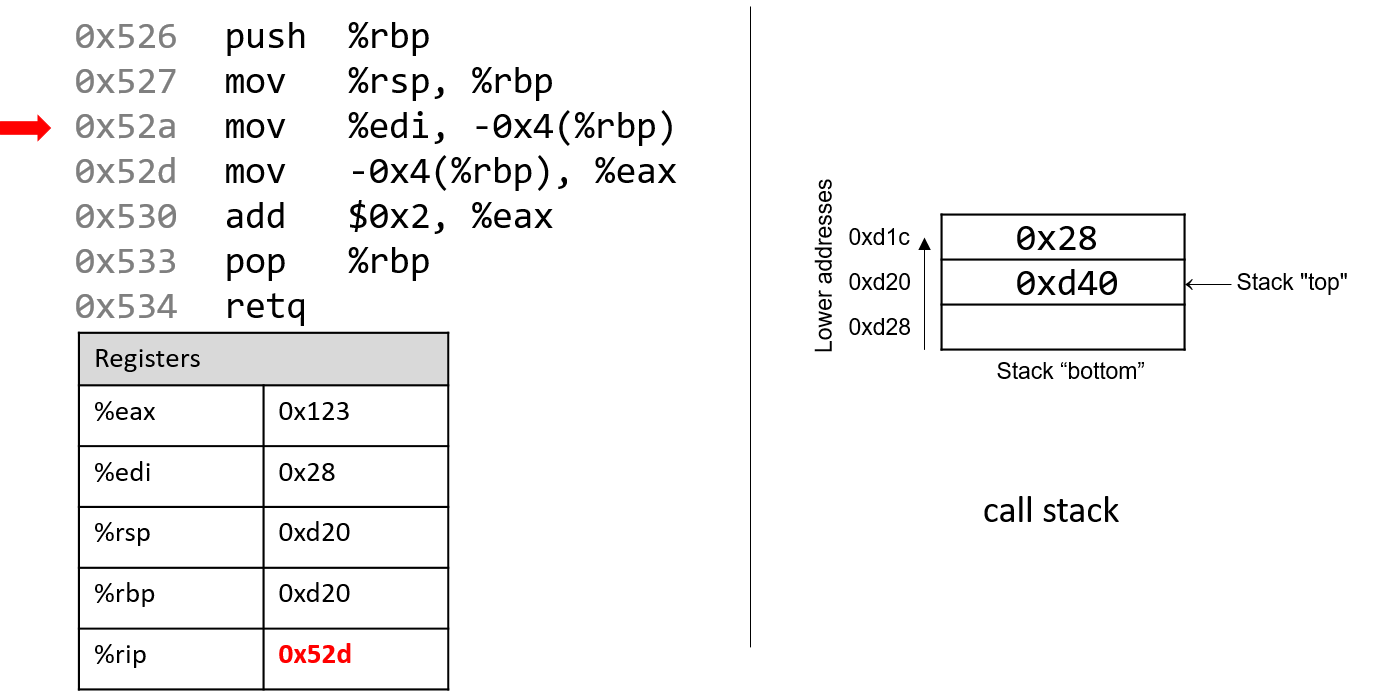
\includegraphics[scale=0.5]{img/ex1_4.png}
            \end{center}

          \item The next instruction simply goes into memory 4 bytes below the stack pointer, takes the value there, and stores it into \texttt{\%eax}. This is the value of \texttt{\%edi} that we just stored. This may seem redundant since we are making a round trip to memory and back to ultimately move the value of \texttt{\%edi} into \texttt{\%eax}, but compilers are not smart and just follow these instructions. 

            \begin{center}
              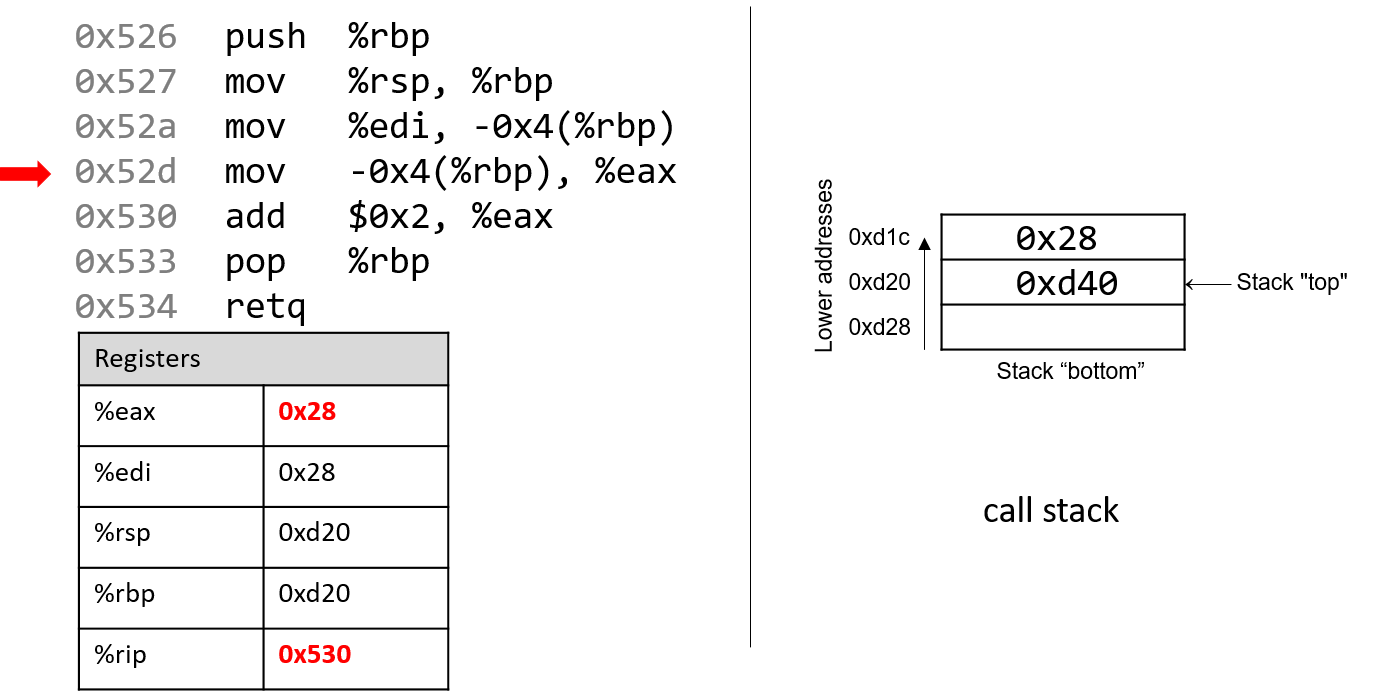
\includegraphics[scale=0.5]{img/ex1_5.png}
            \end{center}

          \item Finally, we add the value \texttt{\$0x2} to \texttt{\%eax} and store it back into \texttt{\%eax}. 

            \begin{center}
              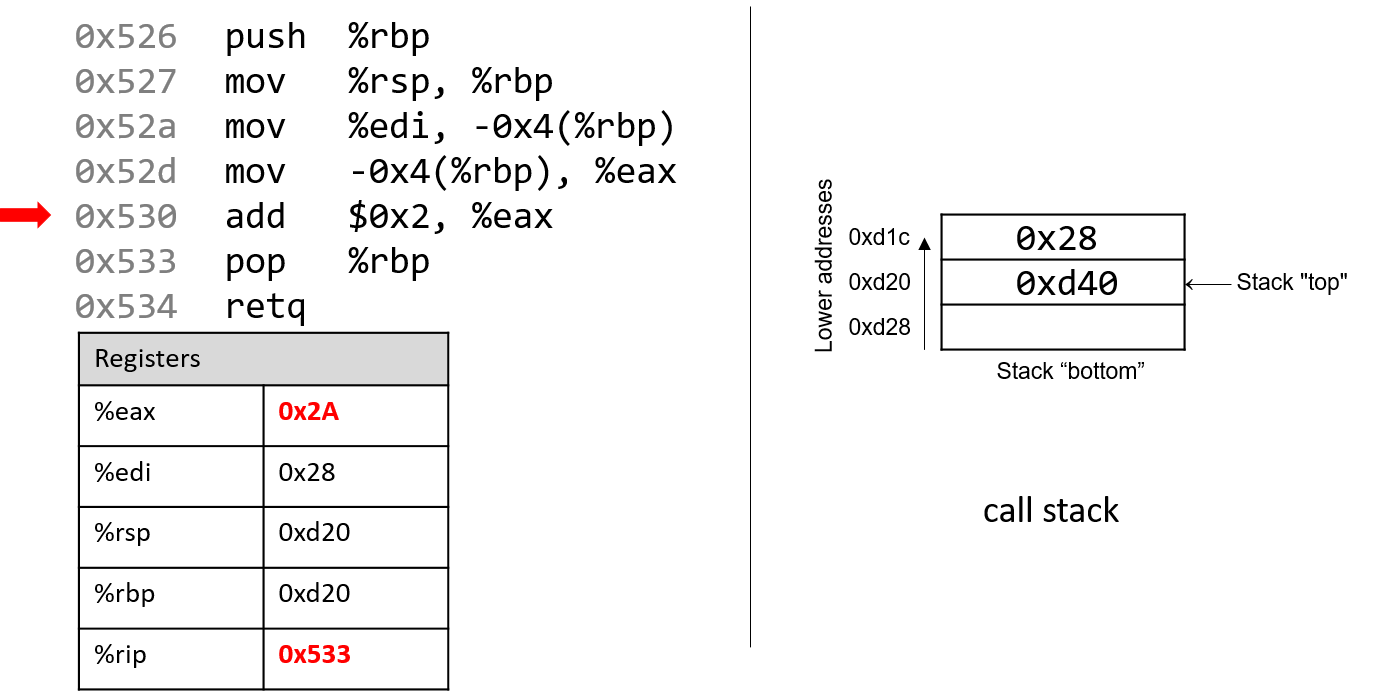
\includegraphics[scale=0.5]{img/ex1_6.png}
            \end{center}

          \item Finally, we pop the value at the top of the stack and store it into \texttt{\%rbp}. Note that this is \textit{not} the value \texttt{0x28}. It is simply the value that is stored at \texttt{\%rsp=0xd20}, which is \texttt{(\%rsp)=0xd40}. 

            \begin{center}
              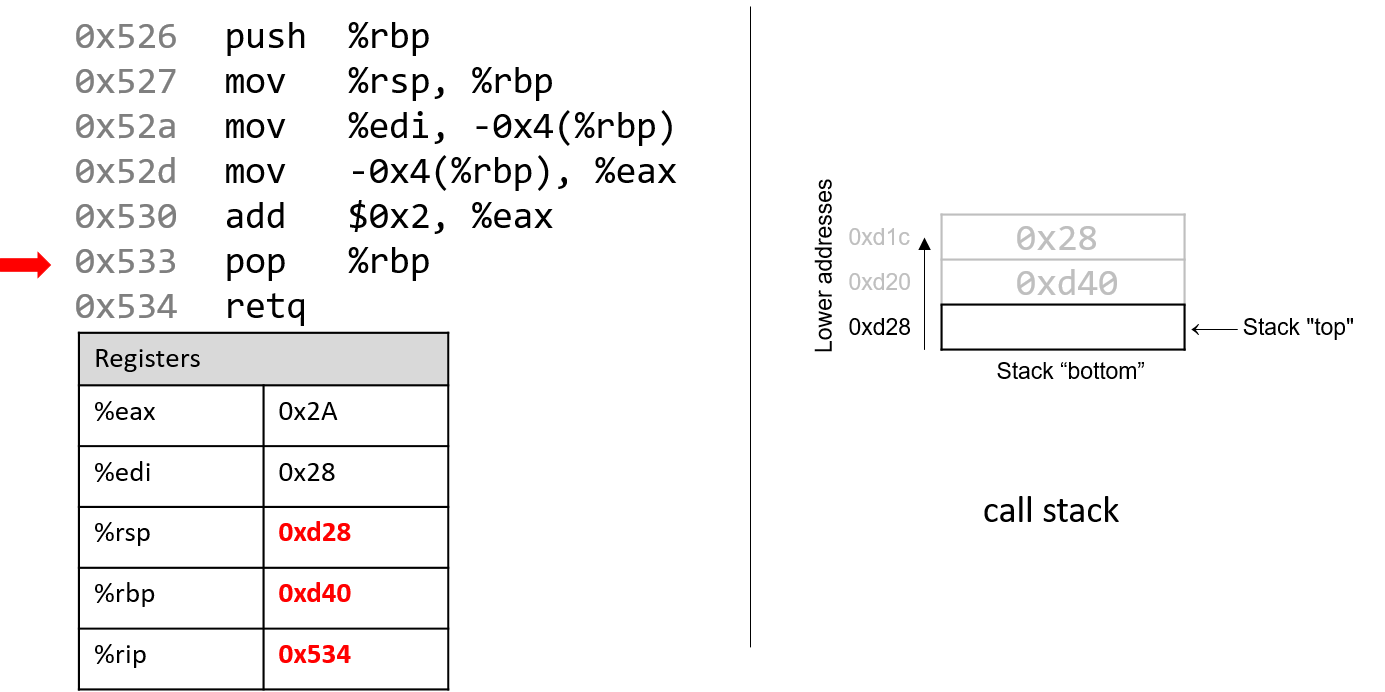
\includegraphics[scale=0.5]{img/ex1_7.png}
            \end{center}

          \item Finally, we return the value with \texttt{retq}. 
        \end{enumerate}
      \end{example}

      Note that the final values in the registers \texttt{\%rsp} and \texttt{\%rip} are \texttt{0xd28} and \texttt{0x534}, respectively, which are the same values as when the function started executing! This is normal and expected behavior with the call stack, which just stores temporary variable sand data of each function as it executes a program. Once a function completes executing, the stack returns to the state it was in prior to the function call. Therefore, it is common to see the following two instructions at the beginning of a function: 
      \begin{lstlisting}
        push %rbp 
        mov %rsp, %rbp
      \end{lstlisting}
      and the following two at the end of a function 
      \begin{lstlisting}
        pop %rbp 
        retq
      \end{lstlisting}

    \subsubsection{Arithmetic Operations}

      \begin{definition}[Add, Subtract, Multiply]
        The \textbf{add} and \textbf{sub} instructions are used to add and subtract data from the destination. 
        \begin{align*}
          \texttt{add\_ src, dest} && \texttt{dest = dest + src} \\
          \texttt{sub\_ src, dest} && \texttt{dest = dest - src}
        \end{align*}
        The \textbf{imul} instruction is used to multiply data between the source and destination and store it in the destination.  
        \begin{align*}
          \texttt{imul\_ src, dest} && \texttt{dest = dest * src} 
        \end{align*}
        Again the \texttt{\_} is a size operand, which determines how big the data is. 
      \end{definition}

      \begin{definition}[Increment, Decrement]
        The \textbf{inc} and \textbf{dec} instructions are used to increment and decrement the value in the destination. 
        \begin{align*}
          \texttt{inc\_ dest} && \texttt{dest = dest + 1} \\
          \texttt{dec\_ dest} && \texttt{dest = dest - 1}
        \end{align*}
      \end{definition}

      \begin{definition}[Negative]
        The \textbf{neg} instruction is used to negate the value in the destination. 
        \begin{align*}
          \texttt{neg\_ dest} && \texttt{dest = -dest} 
        \end{align*}
      \end{definition}

      \begin{example}[Basic Arithmetic Function]
        The following represents the same program in C and in assembly. Let's go through each one: 
        \begin{enumerate}
          \item In C, we first initialize \texttt{a = 4}, then \texttt{b = 8}, add them together to get \texttt{c}, and then return \texttt{c}.
          \item In Assembly, we move the value $4$ to the \texttt{\%rax} register, then move the value $8$ to the \texttt{\%rbx} register, add the two values together to store it into \texttt{\%rax}, and then return the value in the \texttt{\%rax} register.
        \end{enumerate}
        \noindent\begin{minipage}{.5\textwidth}
        \begin{lstlisting}[]{Code}
          int main() {
            int a = 4, b = 8; 
            int c = a + b; 
            return c; 
          }
        \end{lstlisting}
        \end{minipage}
        \hfill
        \begin{minipage}{.49\textwidth}
        \begin{lstlisting}[]{Output}
          main:
            movq $4, %rax
            movq $8, %rbx
            addq %rbx, %rax
            ret
        \end{lstlisting}
        \end{minipage}
        It is slightly different in Assembly since rather than storing $4$ in some intermediate register, we immediately store it in the return register. In a way it is more optimized, and this is what the compiler does for you so that as few registers are used. 
      \end{example}

      A shorthand way to do this is with \texttt{lea}, which stands for load effective address. 

      \begin{definition}[Load Effective Address]
        The \textbf{lea} instruction is used to load the effective address of the source into the destination. For now, we will focus on the arithmetic operations that it can do
        \begin{align*}
          \texttt{lea\_ (src1, src2), dest} && \texttt{dest = src1 + src2}  \\ 
          \texttt{lea\_ (src1, src2, scale), dest} && \texttt{dest = src1 + src2*scale}  \\ 
          \texttt{lea\_ const(src1, src2), dest} && \texttt{dest = src1 + src2 + const} \\ 
          \texttt{lea\_ const(src1, src2, scale), dest} && \texttt{dest = src1 + src2*scale + const}
        \end{align*}
        This is useful for doing arithmetic operations on the address of a variable.
      \end{definition}

      \begin{definition}[Bitwise]
        The \textbf{and}, \textbf{or}, \textbf{xor}, and \textbf{not} instructions are used to perform bitwise operations on the source and destination. 
        \begin{align*}
          \texttt{and src, dest} && \texttt{dest = dest \& src}  \\
          \texttt{or src, dest} && \texttt{dest = dest | src}  \\
          \texttt{xor src, dest} && \texttt{dest = dest \^ src}  \\
          \texttt{neg dest} && \texttt{dest = -dest}  \\
          \texttt{not dest} && \texttt{dest = $\sim$dest}  
        \end{align*}
      \end{definition}

      \begin{definition}[Arithmetic and Logical Bit Shift]
        The \texttt{sal} arithmetic instruction is used to shift the bits of the destination to the left by the number of bits specified in the source. The \texttt{shr} instruction is used to shift the bits of the destination to the right by the number of bits specified in the source.
        \begin{align*}
          \texttt{sal src, dest} && \texttt{dest = dest << src}  \\
          \texttt{shr src, dest} && \texttt{dest = dest >> src}
        \end{align*}
        The \texttt{sar} instruction is used to shift the bits of the destination to the right by the number of bits specified in the source, and fill the leftmost bits with the sign bit. The \texttt{shl} instruction is used to shift the bits of the destination to the left by the number of bits specified in the source, and fill the rightmost bits with zeros. 
        \begin{align*}
          \texttt{sar src, dest} && \texttt{dest = dest >> src}  \\
          \texttt{shl src, dest} && \texttt{dest = dest << src}
        \end{align*}
      \end{definition}

      \begin{example}[Harder Arithmetic Example]
        The following two codes are equivalent. 

        \noindent\begin{minipage}{.5\textwidth}
        \begin{lstlisting}[]{Code}
          long arith(long x, long y, long z) {
            long t1 = x + y; 
            long t2 = z + t1; 
            long t3 = x + 4; 
            long t4 = y * 48; 
            long t5 = t3 + t4;
            long rval = t2 * t5; 
            return rval; 
          }
          .
          .
          .
          .
          .
        \end{lstlisting}
        \end{minipage}
        \hfill
        \begin{minipage}{.49\textwidth}
        \begin{lstlisting}[]{Output}
          arith: 
            # rax/t1 = x + y
            leaq  (%rdi, %rsi), %rax
            # rax/t2 = z + t1
            addq  %rdx, %rax
            #rdx = 3 * y 
            leaq  (%rsi, %rsi, 2), %rdx
            #rdx/t4 = (3*y) * 16
            salq  $4, %rdx 
            #rcx/t5 = x + t4 + 4
            leaq  4(%rdi, %rdi), %rcx 
            # rax/rval = t5 * t2
            imulq %rcx, %rax 
            ret 
        \end{lstlisting}
        \end{minipage}
      \end{example}
    
    \subsubsection{Condition Codes}

      Sometimes, we want to move (really copy) some value to another register if some condition is met. This is where we use conditional moves. These conditions are met by the flags register, which is a special register that stores the status of the last operation. It is the value of these flags that determine whether all future conditional statements are met in assembly. 
      
      \begin{definition}[Condition Code Flags]
        The flags register in the x86 CPU keeps 4 \textit{condition code} flag bits internally. Think of these as status flags that are \textit{implicitly} set by the most recent arithmetic operation (think of it as side effects). Note that condition codes are NOT set by \texttt{lea} or \texttt{mov} instructions! 
        \begin{enumerate}
          \item \textbf{Zero Flag}: if the last operation resulted in a zero value.
          \item \textbf{Sign Flag}: if the last operation resulted in a negative value (i.e. the most significant bit is 1).
          \item \textbf{Overflow Flag}: if the last operation resulted in a signed overflow.
          \item \textbf{Carry Flag}: if the last operation resulted in a carry out of the most significant bit, i.e. an unsigned overflow. 
        \end{enumerate}
        Every operation may or may not changes these flags to test for zero or nonzero, positive or negative, or overflow conditions, and combinations of these flags express the full range of conditions and cases, e.g. for signed and unsigned values. 
      \end{definition}

      \begin{example}[Zero Flag]
        If the code below was just run, then ZF would be set to 1. 
        \begin{lstlisting}
          movq $2, %rax 
          subq $2, %rax
        \end{lstlisting}
      \end{example}

      \begin{example}[Sign Flag]
        If the code below was just run, then SF would be set to 1. 
        \begin{lstlisting}
          movq $2, %rax 
          subq $4, %rax
        \end{lstlisting}
      \end{example}

      \begin{example}[Overflow Flag]
        If either code below was just run, then OF would be set to 1. 

        \noindent\begin{minipage}{.5\textwidth}
        \begin{lstlisting}[]{Code}
          movq $0x7fffffffffffffff, %rax 
          addq $1, %rax
        \end{lstlisting}
        \end{minipage}
        \hfill
        \begin{minipage}{.49\textwidth}
        \begin{lstlisting}[]{Output}
          movq 0x8000000000000000, %rax 
          addq 0xffffffffffffffff, %rax
        \end{lstlisting}
        \end{minipage}
        This is because in the left in signed arithmetic, we have a positive + positive = negative (result is \texttt{0x8000000000000000}), which is a signed overflow. Furthermore, in the right we have negative + negative = positive (result is \texttt{0x7fffffffffffffff}). 
      \end{example}

      \begin{example}[Carry Flag]
        If the code below was just run, then CF would be set to 1. 
        \begin{lstlisting}
          movq $0xffffffffffffffff, %rax 
          addq $1, %rax
        \end{lstlisting}
        This is because the result is $0x0$, which is a carry out of the most significant bit and an unsigned overflow.
      \end{example}

      It would be tedious to always set these flags manually, so there are two methods that can be used to \textit{explicitly} set these flags. 

      \begin{definition}[Compare]
        The \textbf{cmp} instruction is used to perform a subtraction between the source and destination, and set the flags accordingly, but it does not store the result.
        \begin{align*}
          \texttt{cmp\_ src, dest} && \texttt{dest - src} 
        \end{align*}
        The following flags are set if the conditions are met: 
        \begin{enumerate}
          \item \textbf{ZF = 1} if \texttt{dest == src} 
          \item \textbf{SF = 1} if \texttt{dest < src} (MSB is 1) 
          \item \textbf{OF = 1} if signed overflow 
          \item \textbf{CF = 1} if unsigned overflow
        \end{enumerate}
      \end{definition}

      \begin{definition}[Test]
        The \textbf{test} instruction is used to perform a bitwise AND operation between the source and destination, and set the flags accordingly. 
        \begin{align*}
          \texttt{test\_ src, dest} && \texttt{dest \& src} 
        \end{align*}
        The following flags are set if the conditions are met. Note that you can't have carry out (CF) or overflow (OF) if these flags are set. 
        \begin{enumerate}
          \item \textbf{ZF = 1} if \texttt{dest \& src == 0} 
          \item \textbf{SF = 1} if \texttt{dest \& src < 0} (MSB is 1) 
        \end{enumerate}
      \end{definition}

      \begin{example}[Compare] 
        Assuming that \texttt{\%al = 0x80} and \texttt{\%bl = 0x81}, which flags are set when we execute \texttt{cmpb \%al, \%bl}? Well we must first compute 
        \begin{equation}
          \texttt{\%bl - \%al = 0x81 - 0x80 = 0x81 + $\sim$ 0x80 + 1 = 0x81 + 0x7F + 1 = 0x101 = 0x01}
        \end{equation}
        \begin{enumerate}
          \item CF=1 since the result is greater than 0xFF (i.e. larger than byte) 
          \item ZF=0 since the result is not 0 
          \item SF=0 since the MSB is 0, i.e. there is unsigned overflow
          \item OF=0 since there is no signed overflow
        \end{enumerate}
      \end{example}

      For conditional moves and jumps later shown, it basically uses these explicit sets and always compares them to $0$. We will see what this means later. 

      Finally, we can actually set a byte in a register to 1 or 0 based on the value of a flag. 

      \begin{definition}[Set]
        
      \end{definition}

    \subsubsection{Conditional Move and Jumps}
    
      \begin{definition}[Equality with 0]
        The \texttt{test} instruction is used to perform a bitwise AND operation between the source and destination, and set the flags accordingly. 
        \begin{align*}
          \texttt{test\_ src, dest} && \texttt{dest \& src} 
        \end{align*}
        The \texttt{sete} instruction is used to set the destination to 1 if the zero flag is set, and 0 otherwise. 
        \begin{align*}
          \texttt{sete\_ dest} && \texttt{dest = (ZF == 1) ? 1 : 0} 
        \end{align*}
        The \texttt{cmovne} instruction is used to move the source to the destination if the zero flag is not set. 
        \begin{align*}
          \texttt{cmovne\_ src, dest} && \texttt{dest = (ZF == 0) ? src : dest} 
        \end{align*}
      \end{definition}


      \begin{definition}[Jump]
        There are several jump instructions, but essentially they are used to jump to another part of the code. We can use the following mnemonic to jump to a label. 

        \begin{figure}[H]
          \centering 
          \begin{table}[H]
            \centering
            \begin{tabular}{|l|l|}
            \hline
            \textbf{Letter} & \textbf{Word} \\ \hline
            j & jump \\ \hline
            n & not \\ \hline
            e & equal \\ \hline
            s & signed \\ \hline
            g & greater (signed interpretation) \\ \hline
            l & less (signed interpretation) \\ \hline
            a & above (unsigned interpretation) \\ \hline
            b & below (unsigned interpretation) \\ \hline
            \end{tabular}
            \caption{Letter to Word Mapping}
            \label{table:letter_word_mapping}
          \end{table}
          \caption{Mnemonic for Jump Instructions} 
          \label{fig:jump_instructions_mnemonic}
        \end{figure}

        For completeness, we include all the jump instructions. 
          
        \begin{figure}[H]
          \centering 
          \begin{table}[H]
            \centering
            \begin{tabular}{|l|l|l|}
            \hline
            \textbf{Signed Comparison} & \textbf{Unsigned Comparison} & \textbf{Description} \\ \hline
            je (jz) & & jump if equal (==) or jump if zero \\ \hline
            jne (jnz) & & jump if not equal (!=) \\ \hline
            js & & jump if negative \\ \hline
            jns & & jump if non-negative \\ \hline
            jg (jnle) & ja (jnbe) & jump if greater (>) \\ \hline
            jge (jnl) & jae (jnb) & jump if greater than or equal (>=) \\ \hline
            jl (jnge) & jb (jnae) & jump if less (<) \\ \hline
            jle (jng) & jbe (jna) & jump if less than or equal (<=) \\ \hline
            \end{tabular}
            \caption{Comparison Instructions in Assembly}
            \label{table:comparison_instructions}
          \end{table}
          \caption{All jump instructions} 
          \label{fig:jump_instructions_all}
        \end{figure}
      \end{definition}

      \begin{definition}[int]
        The \texttt{int} instruction is used to generate a software interrupt. It is often used to invoke a system call.
      \end{definition}

      \begin{definition}[ret]
        The \texttt{ret} instruction is used to return from a function. It returns the value in the \texttt{\%rax} register. 
      \end{definition}

    \subsubsection{If Statements}

      Now we can have a basic idea of how if statements can be used as a sequence of conditionals and jump operators. Let's first look at the \textbf{goto} version of C. 

      \begin{definition}[Goto Syntax]
        The goto version processes instructions sequentially as long as there is no jump. This is useful because compilers translating code into assembly designate a jump when a condition is true. Contrast this behavior with the structure of an if statement, where a "jump" (to the else) occurs when conditions are not true. The goto form captures this difference in logic.
      \end{definition}

      \begin{figure}[H]
        \centering 
        \noindent\begin{minipage}{.5\textwidth}
        \begin{lstlisting}[]{Code}
          int getSmallest(int x, int y) {
            int smallest;
            if ( x > y ) { //if (conditional)
              smallest = y; //then statement
            }
            else {
              smallest = x; //else statement
            }
            return smallest;
          }
          .
          .
          .
          .
          .
        \end{lstlisting}
        \end{minipage}
        \hfill
        \begin{minipage}{.49\textwidth}
        \begin{lstlisting}[]{Output}
          int getSmallest(int x, int y) {
            int smallest;

            if (x <= y ) { //if (!conditional)
              goto else_statement;
            }
            smallest = y; //then statement
            goto done;

          else_statement:
            smallest = x; //else statement

          done:
            return smallest;
          }      
        \end{lstlisting}
        \end{minipage}
        \caption{C vs GoTo code of the same function. While GoTo code allows us to view C more like assmebly, it is generally not readable and is not considered best practice. } 
        \label{fig:c_vs_goto}
      \end{figure}

      Now let's see how if statements are implemented by taking a look at this function straight up in assembly. 

      \begin{figure}[H]
        \centering 
        \noindent\begin{minipage}{.4\textwidth}
        \begin{lstlisting}[]{Code}
          int getSmallest(int x, int y) {
            int smallest;
            if ( x > y ) { //if (conditional)
              smallest = y; //then statement
            }
            else {
              smallest = x; //else statement
            }
            return smallest;
          }
          .
        \end{lstlisting}
        \end{minipage}
        \hfill
        \begin{minipage}{.59\textwidth}
        \begin{lstlisting}[]{Output}
          Dump of assembler code for function getSmallest:
          0x40059a <+4>:   mov    %edi,-0x14(%rbp)
          0x40059d <+7>:   mov    %esi,-0x18(%rbp)
          0x4005a0 <+10>:  mov    -0x14(%rbp),%eax
          0x4005a3 <+13>:  cmp    -0x18(%rbp),%eax
          0x4005a6 <+16>:  jle    0x4005b0 <getSmallest+26>
          0x4005a8 <+18>:  mov    -0x18(%rbp),%eax
          0x4005ae <+24>:  jmp    0x4005b9 <getSmallest+35>
          0x4005b0 <+26>:  mov    -0x14(%rbp),%eax
          0x4005b9 <+35>:  pop    %rbp
          0x4005ba <+36>:  retq
        \end{lstlisting}
        \end{minipage}
        \caption{Assembly code of a simple if statement} 
        \label{fig:if_statement}
      \end{figure}

      Again, note that since we are working with int types, the respective parameter registers are \texttt{\%edi} and \texttt{\%esi}, the respective lower 32-bits of the registers \texttt{\%rdi} and \texttt{\%rsi}. Let's walk through this again. 
      \begin{enumerate}
        \item The first mov instruction copies the value located in register \%edi (the first parameter, x) and places it at memory location \%rbp-0x14 on the call stack. The instruction pointer (\%rip) is set to the address of the next instruction, or 0x40059d.
        \item The second mov instruction copies the value located in register \%esi (the second parameter, y) and places it at memory location \%rbp-0x18 on the call stack. The instruction pointer (\%rip) updates to point to the address of the next instruction, or 0x4005a0.
        \item The third mov instruction copies x to register \%eax. Register \%rip updates to point to the address of the next instruction in sequence.
        \item The cmp instruction compares the value at location \%rbp-0x18 (the second parameter, y) to x and sets appropriate condition code flag registers. Register \%rip advances to the address of the next instruction, or 0x4005a6.
        \item The jle instruction at address 0x4005a6 indicates that if x is less than or equal to y, the next instruction that should execute should be at location <getSmallest+26> and that \%rip should be set to address 0x4005b0. Otherwise, \%rip is set to the next instruction in sequence, or 0x4005a8.
      \end{enumerate}

      With the \texttt{cmov} instruction, this can be a lot shorter. With the gcc compiler with level 1 optimizations turned on, we can see that a lot of redundancies are turned off. 

      \begin{figure}[H]
        \centering 
        \begin{lstlisting}
          <getSmallest>:
          0x400546 <+0>: cmp    %esi,%edi      #compare x and y
          0x400548 <+2>: mov    %esi,%eax      #copy y to %eax
          0x40054a <+4>: cmovle %edi,%eax      #if (x<=y) copy x to %eax
          0x40054d <+7>: retq                  #return %eax
        \end{lstlisting}
        \caption{Compiled with \texttt{gcc -01 -o getSmallest getSmallest.c} } 
        \label{fig:if_statement_optimized}
      \end{figure}

    \subsubsection{Loops}
      
      Like if statements, loops in assembly can be implementing using jump functions that revisit some instruction address based on the result on an evaluated condition. Let's take a look at a basic loop function. 

      \begin{figure}[H]
        \centering 
        \noindent\begin{minipage}{.5\textwidth}
        \begin{lstlisting}[]{Code}
          int sumUp(int n) {
            int total = 0;
            int i = 1;

            while (i <= n) {  
              total += i;   
              i++; 
            }
            return total;
          }
          .
          .
          .
          .
          .
          .
        \end{lstlisting}
        \end{minipage}
        \hfill
        \begin{minipage}{.49\textwidth}
        \begin{lstlisting}[]{Output}
          Dump of assembler code for function sumUp:
          0x400526 <+0>:   push   %rbp
          0x400527 <+1>:   mov    %rsp,%rbp
          0x40052a <+4>:   mov    %edi,-0x14(%rbp)
          0x40052d <+7>:   mov    $0x0,-0x8(%rbp)
          0x400534 <+14>:  mov    $0x1,-0x4(%rbp)
          0x40053b <+21>:  jmp    0x400547 <sumUp+33>
          0x40053d <+23>:  mov    -0x4(%rbp),%eax
          0x400540 <+26>:  add    %eax,-0x8(%rbp)
          0x400543 <+29>:  add    $0x1,-0x4(%rbp)
          0x400547 <+33>:  mov    -0x4(%rbp),%eax
          0x40054a <+36>:  cmp    -0x14(%rbp),%eax
          0x40054d <+39>:  jle    0x40053d <sumUp+23>
          0x40054f <+41>:  mov    -0x8(%rbp),%eax
          0x400552 <+44>:  pop    %rbp
          0x400553 <+45>:  retq
        \end{lstlisting}
        \end{minipage}
        \caption{Simple loop function in C and assembly. } 
        \label{fig:loop_function}
      \end{figure}

    \subsubsection{Functions}

      So far, we've traced through simple functions in assembly. n this section, we discuss the interaction between multiple functions in assembly in the context of a larger program. We also introduce some new instructions involved with function management. 

      Let’s begin with a refresher on how the call stack is managed. Recall that \texttt{\%rsp} is the stack pointer and always points to the top of the stack. The register \texttt{\%rbp} represents the base pointer (also known as the frame pointer) and points to the base of the current stack frame. The stack frame (also known as the activation frame or the activation record) refers to the portion of the stack allocated to a single function call. The currently executing function is always at the top of the stack, and its stack frame is referred to as the active frame. The active frame is bounded by the stack pointer (at the top of stack) and the frame pointer (at the bottom of the frame). The activation record typically holds local variables for a function.

      \begin{figure}[H]
        \centering 
        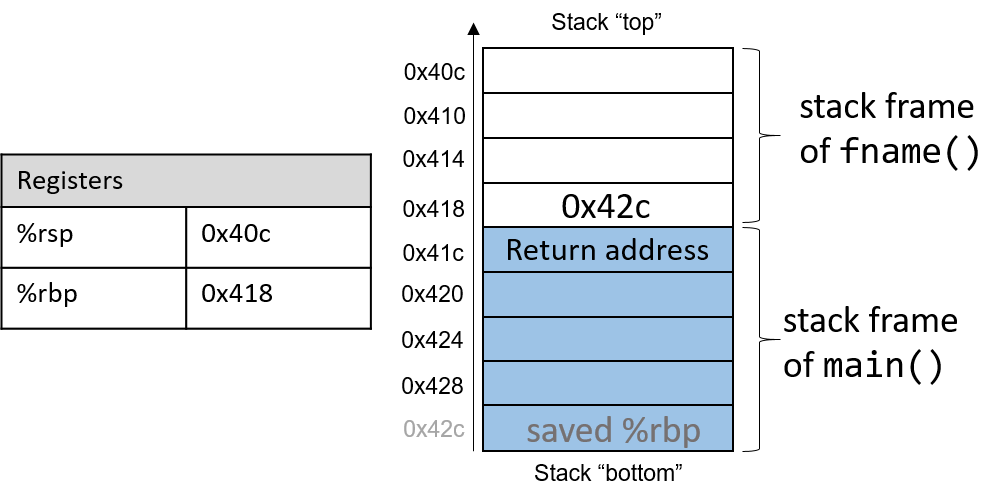
\includegraphics[scale=0.6]{img/stackFrame.png}
        \caption{The current active frame belongs to the callee function (fname). The memory between the stack pointer and the frame pointer is used for local variables. The stack pointer moves as local values are pushed and popped from the stack. In contrast, the frame pointer remains relatively constant, pointing to the beginning (the bottom) of the current stack frame. As a result, compilers like GCC commonly reference values on the stack relative to the frame pointer. In Figure 1, the active frame is bounded below by the base pointer of fname, which is stack address 0x418. The value stored at address 0x418 is the "saved" \texttt{\%rbp} value (0x42c), which itself is an address that indicates the bottom of the activation frame for the main function. The top of the activation frame of main is bounded by the return address, which indicates where in the main function program execution resumes once the callee function fname finishes executing. }
        \label{fig:stack_frame_management}
      \end{figure}

      In here, we introduce three common instructions that are used to manage the call stack. 

      \begin{definition}[Leave]
        The \textbf{leave} instruction is used to deallocate the current stack frame. For example, the leaveq instruction is a shorthand that the compiler uses to restore the stack and frame pointers as it prepares to leave a function. When the callee function finishes execution, leaveq ensures that the frame pointer is restored to its previous value. It is equivalent to the following two instructions: 
        \begin{align*}
          \texttt{leaveq} && \texttt{movq \%rbp, \%rsp} \\
                          && \texttt{popq \%rbp}
        \end{align*}
      \end{definition}
    
      \begin{definition}[Call and Return]
        The \textbf{call} instruction is used to call a function and the \textbf{ret} to return from a function. The callq and retq instructions play a prominent role in the process where one function calls another. Both instructions modify the instruction pointer (register \%rip). 

        \begin{enumerate}
          \item When the caller function executes the callq instruction, the current value of \%rip is saved on the stack to represent the return address, or the program address at which the caller resumes executing once the callee function finishes. The callq instruction also replaces the value of \%rip with the address of the callee function. 
            \begin{align*}
              \texttt{callq addr <fname>} && \texttt{push \%rip} \\
                                          && \texttt{mov addr, \%rip}
            \end{align*}
          \item The retq instruction restores the value of \%rip to the value saved on the stack, ensuring that the program resumes execution at the program address specified in the caller function. Any value returned by the callee is stored in \%rax or one of its component registers (e.g., \%eax). The retq instruction is usually the last instruction that executes in any function.
            \begin{align*}
              \texttt{retq} && \texttt{pop \%rip} \\
            \end{align*}
        \end{enumerate}
      \end{definition}

      Let's work through an example to solidify our knowledge. 

      \begin{example}[Calling Functions in Assembly]
        Let's take the following code and trace through main. 
        \begin{figure}[H]
          \centering 
          \noindent\begin{minipage}{.25\textwidth}
          \begin{lstlisting}[]{Code}
            #include <stdio.h>

            int assign(void) {
                int y = 40;
                return y;
            }

            int adder(void) {
                int a;
                return a + 2;
            }

            int main(void) {
                int x;
                assign();
                x = adder();
                printf("x is: %d\n", x);
                return 0;
            }
            .
            .
            .
            .
            .
            .
            .
            .
            .
            .
            .
            .
          \end{lstlisting}
          \end{minipage}
          \hfill
          \begin{minipage}{.74\textwidth}
          \begin{lstlisting}[]{Output}
            0000000000400526 <assign>:
              400526:       55                      push   %rbp
              400527:       48 89 e5                mov    %rsp,%rbp
              40052a:       c7 45 fc 28 00 00 00    movl   $0x28,-0x4(%rbp)
              400531:       8b 45 fc                mov    -0x4(%rbp),%eax
              400534:       5d                      pop    %rbp
              400535:       c3                      retq

            0000000000400536 <adder>:
              400536:       55                      push   %rbp
              400537:       48 89 e5                mov    %rsp,%rbp
              40053a:       8b 45 fc                mov    -0x4(%rbp),%eax
              40053d:       83 c0 02                add    $0x2,%eax
              400540:       5d                      pop    %rbp
              400541:       c3                      retq

            0000000000400542 <main>:
              400542:       55                      push   %rbp
              400543:       48 89 e5                mov    %rsp,%rbp
              400546:       48 83 ec 10             sub    $0x10,%rsp
              40054a:       e8 e3 ff ff ff          callq  400526 <assign>
              40054f:       e8 d2 ff ff ff          callq  400536 <adder>
              400554:       89 45 fc                mov    %eax,-0x4(%rbp)
              400557:       8b 45 fc                mov    -0x4(%rbp),%eax
              40055a:       89 c6                   mov    %eax,%esi
              40055c:       bf 04 06 40 00          mov    $0x400604,%edi
              400561:       b8 00 00 00 00          mov    $0x0,%eax
              400566:       e8 95 fe ff ff          callq  400400 <printf@plt>
              40056b:       b8 00 00 00 00          mov    $0x0,%eax
              400570:       c9                      leaveq
              400571:       c3                      retq
          \end{lstlisting}
          \end{minipage}
          \caption{C code and its assembly equivalent. Main function calls two other functions. } 
          \label{fig:calling_functions}
        \end{figure}

        Let's trace through what happens here in detail. This will be long. 

        \begin{enumerate}
          \item \texttt{\%rbp} is the base pointer that is initialized to something. Before we even begin main, say that we have the following initializations, where \texttt{\%eax}, \texttt{\%edi} is garbage. \texttt{\%rsp} denotes where on the stack we are right before calling to main, \textbf{\%rbp} is the base pointer to the current program, and \textbf{\%rip} should be the address of the first instruction in main. Again since we work with integers we use the lower 32-bits of the registers. \texttt{\%rip} now points to the next instruction. 
            \begin{center}
              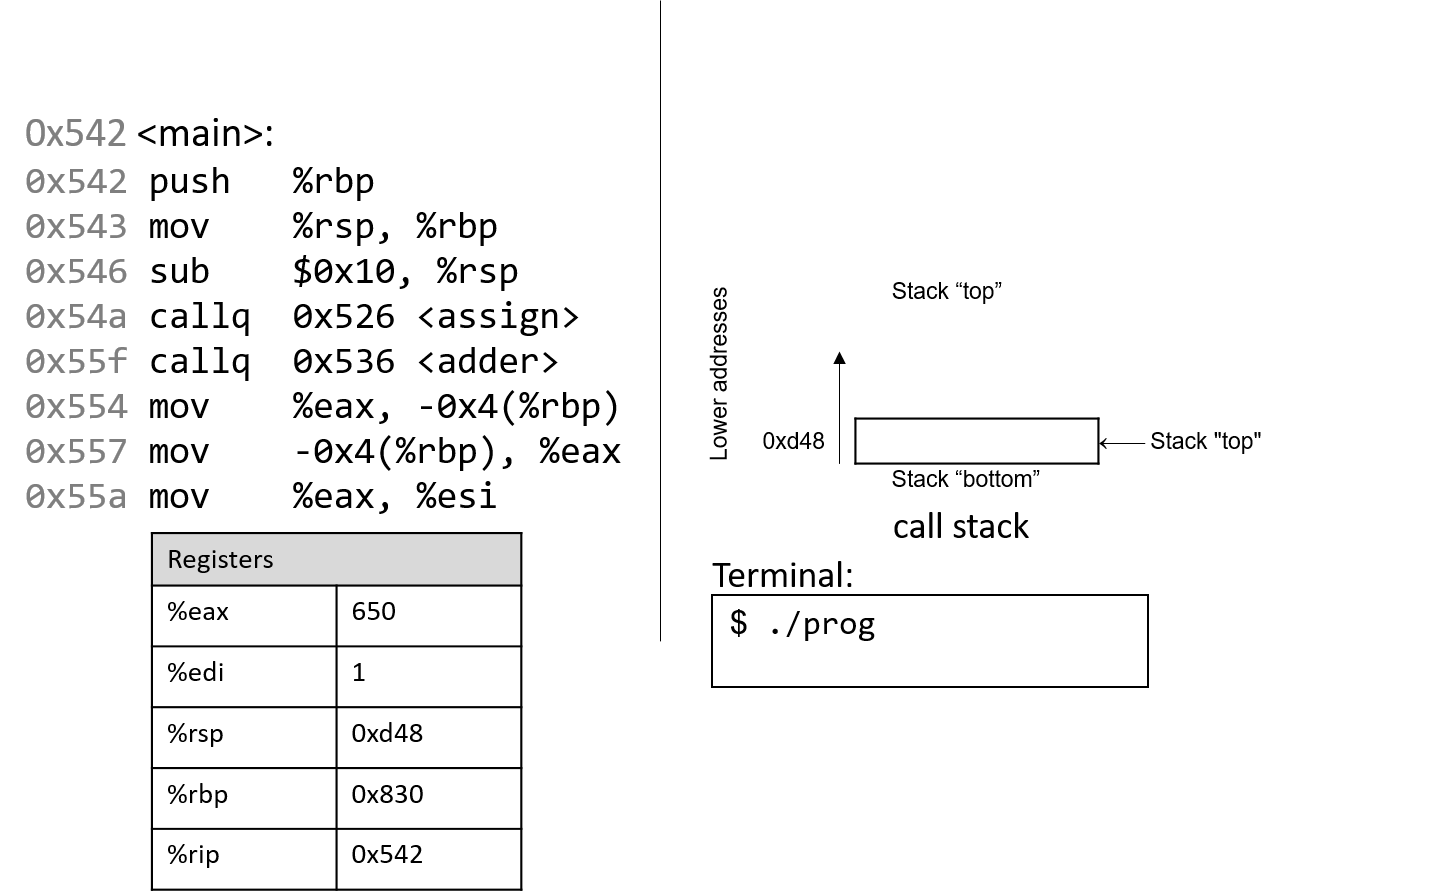
\includegraphics[scale=0.5]{img/Slide1.png}
            \end{center}  

          \item Now we start the main function. By calling main, the base pointer \texttt{\%rbp} of the stack outside of the main frame will be overwritten by the base of the main stack frame, so we must save it for when main is done. Therefore, we push it onto the stack where \texttt{\%rsp} is pointing. \texttt{\%rip} now points to the next instruction. 
            \begin{center}
              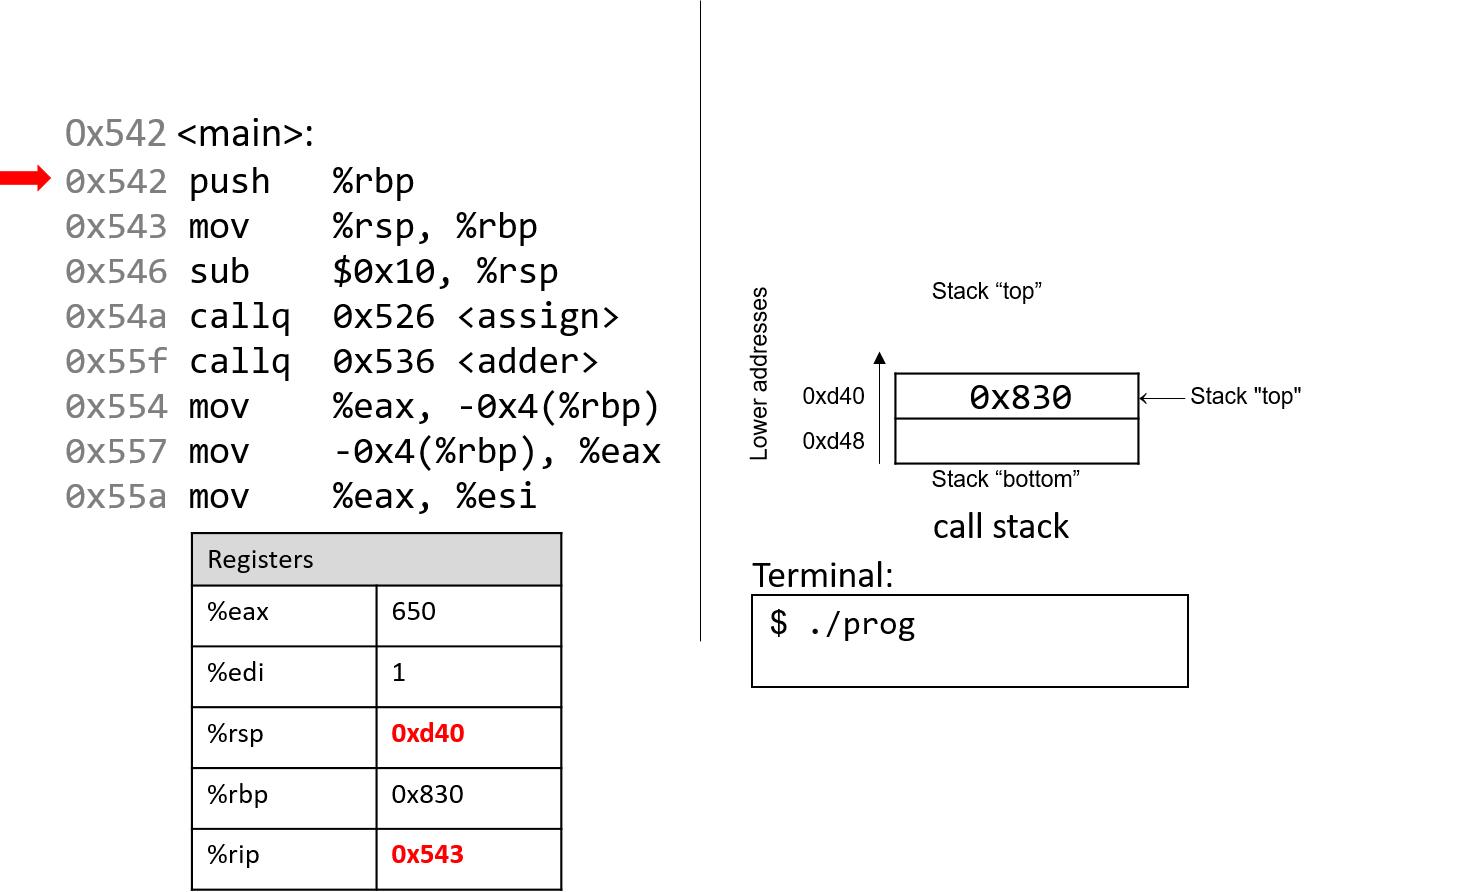
\includegraphics[scale=0.5]{img/Slide2.png}
            \end{center}

          \item Then we actually change the location of the base pointer to the top of the stack, which now includes the first instruction in main. 
            \begin{center}
              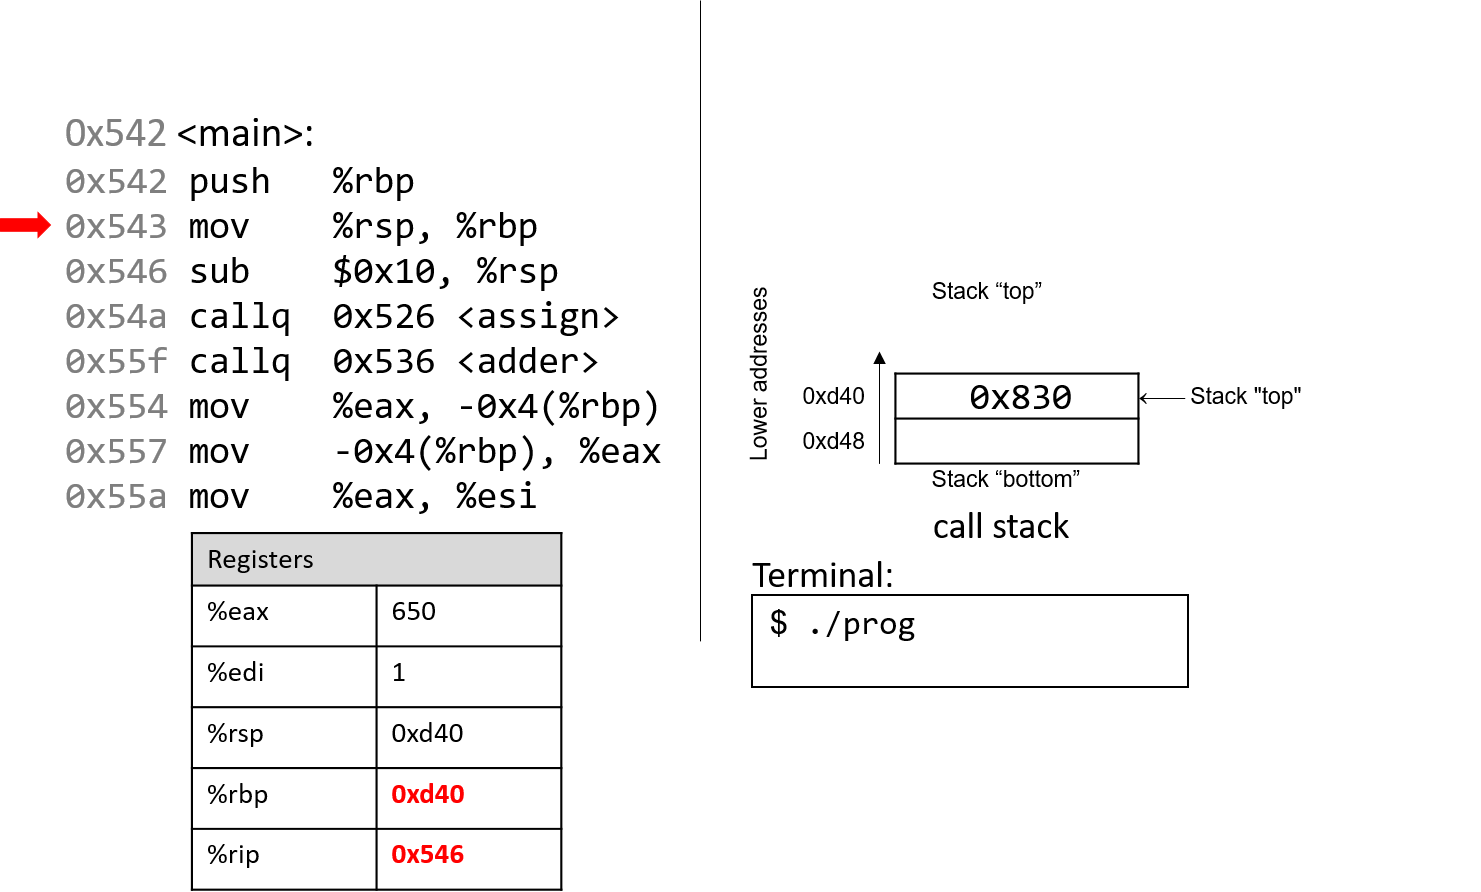
\includegraphics[scale=0.5]{img/Slide3.png}
            \end{center} 

          \item Now we manually change the stack pointer and have it grow by two bytes (\texttt{0x10}). Therefore, \texttt{\%rsp} is decremented by \texttt{0x10} and \texttt{\%rip} points to the next instruction at \texttt{0x54a}. 
            \begin{center}
              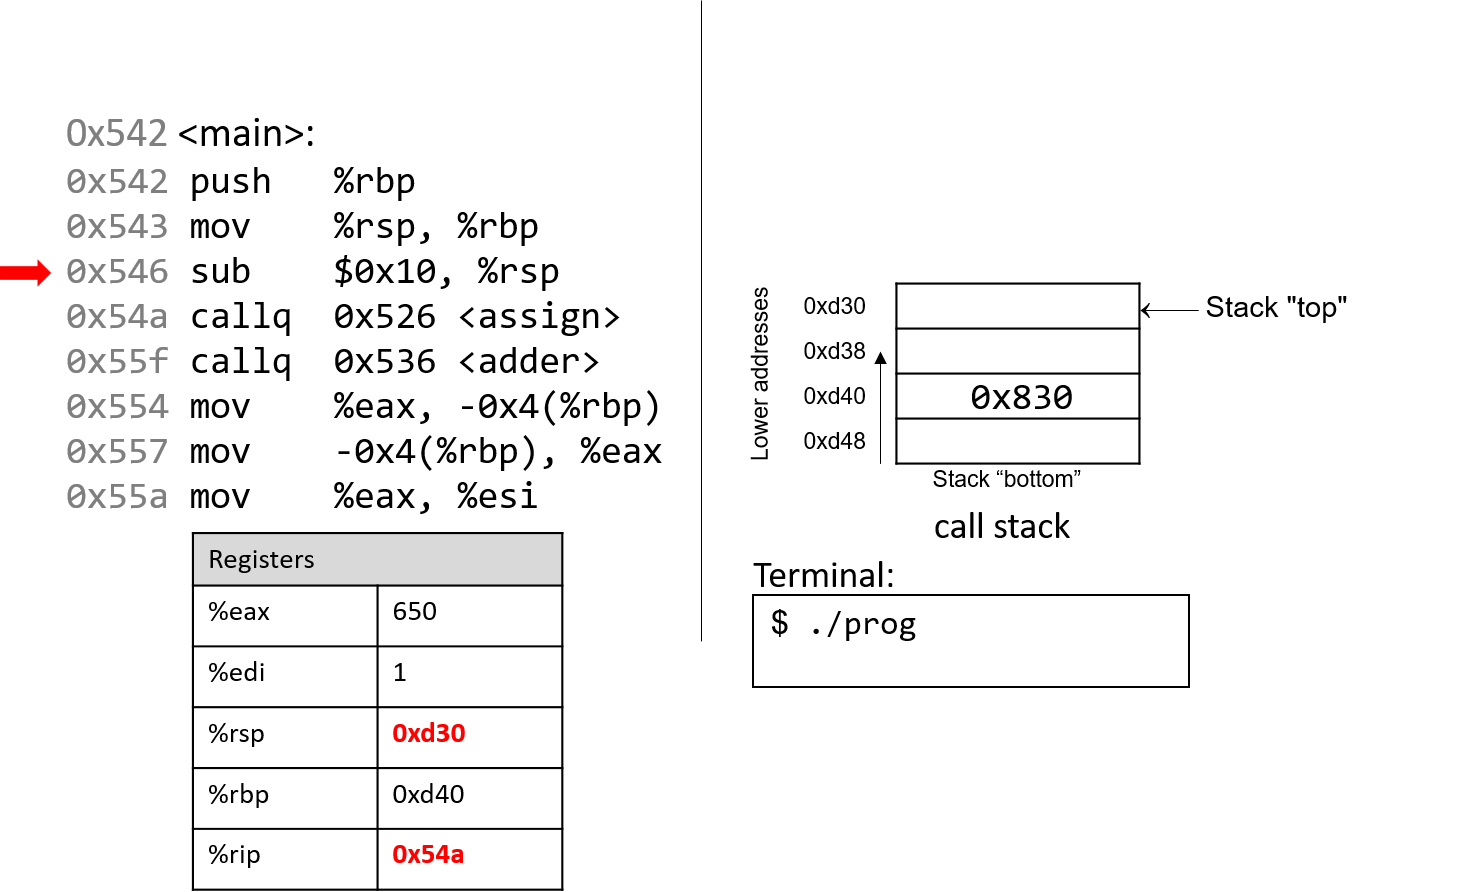
\includegraphics[scale=0.5]{img/Slide4.png}
            \end{center}
            
          \item Now the next instruction pointed at by \texttt{\%rip} is the \texttt{callq} instruction, which tells to go to the address of the \texttt{assign} function. We by default first update \texttt{\%rip} to point to the next instruction at \texttt{0x55f}. However, this should not be the actual next instruction that we execute since we are calling another function. Rather, we want to update \texttt{\%rip} to address \texttt{0x526} where \texttt{assign} is located at, but after completion we also want to know that we want to execute the instruction after it at address \texttt{0x55f}. Therefore, we should \textit{save} address \texttt{0x55f} onto the stack and then update \texttt{\%rip} to point to \texttt{0x526}. This is what we refer to as a \textbf{return address}. 
            \begin{center}
              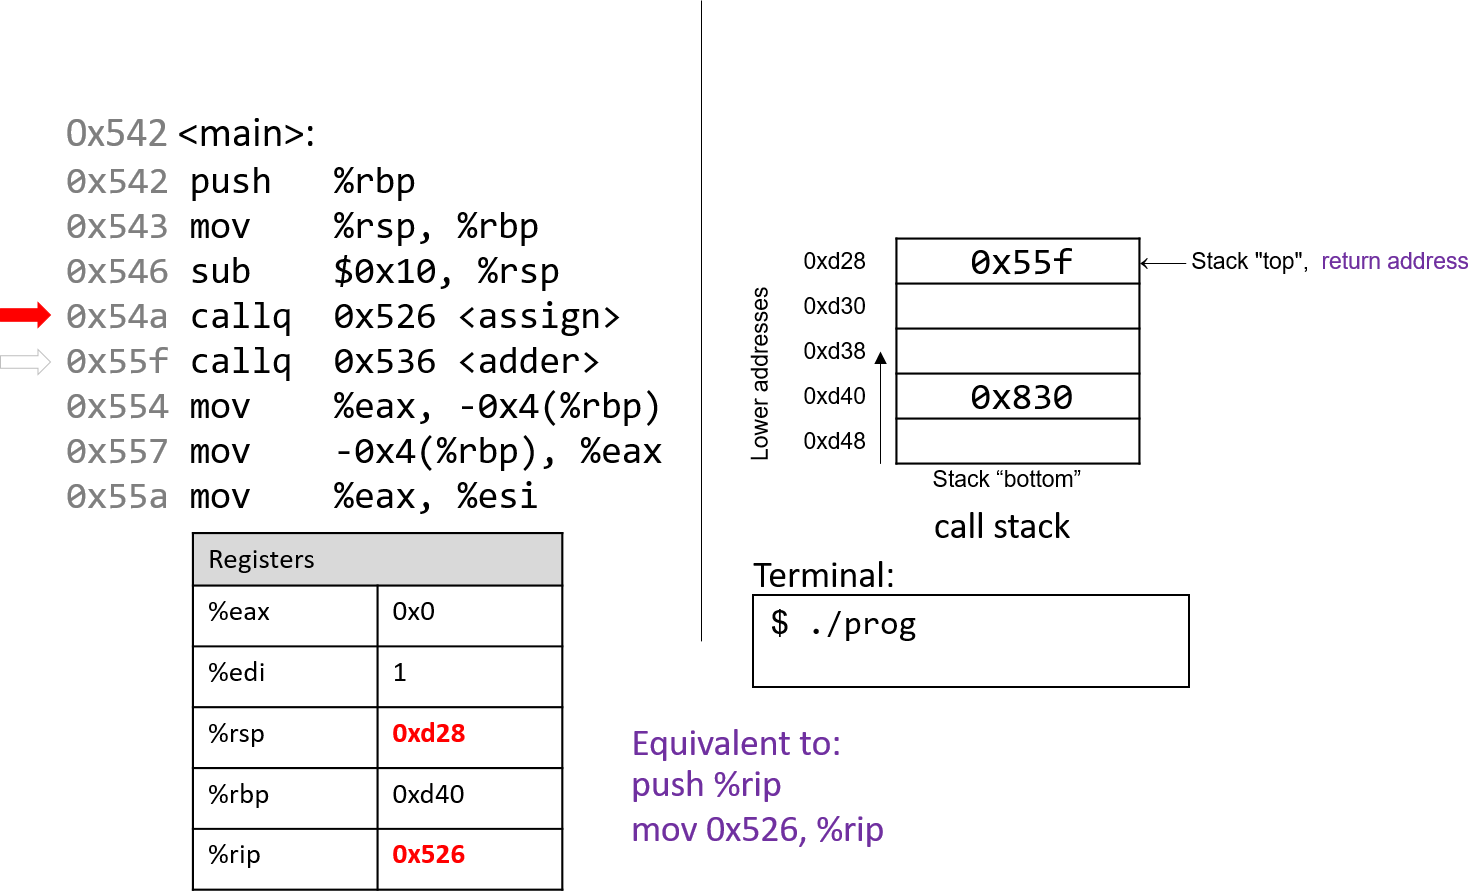
\includegraphics[scale=0.5]{img/Slide5.png}
            \end{center}

          \item \texttt{\%rip} is incremented to the next address. We step into the \texttt{assign} function, which is now a new stack frame, so the first thing we do is save the base pointer of the main stack frame onto the stack since we must immediately update it with the base pointer of the assign stack frame, which is where \texttt{\%rsp} is pointing to. 
            \begin{center}
              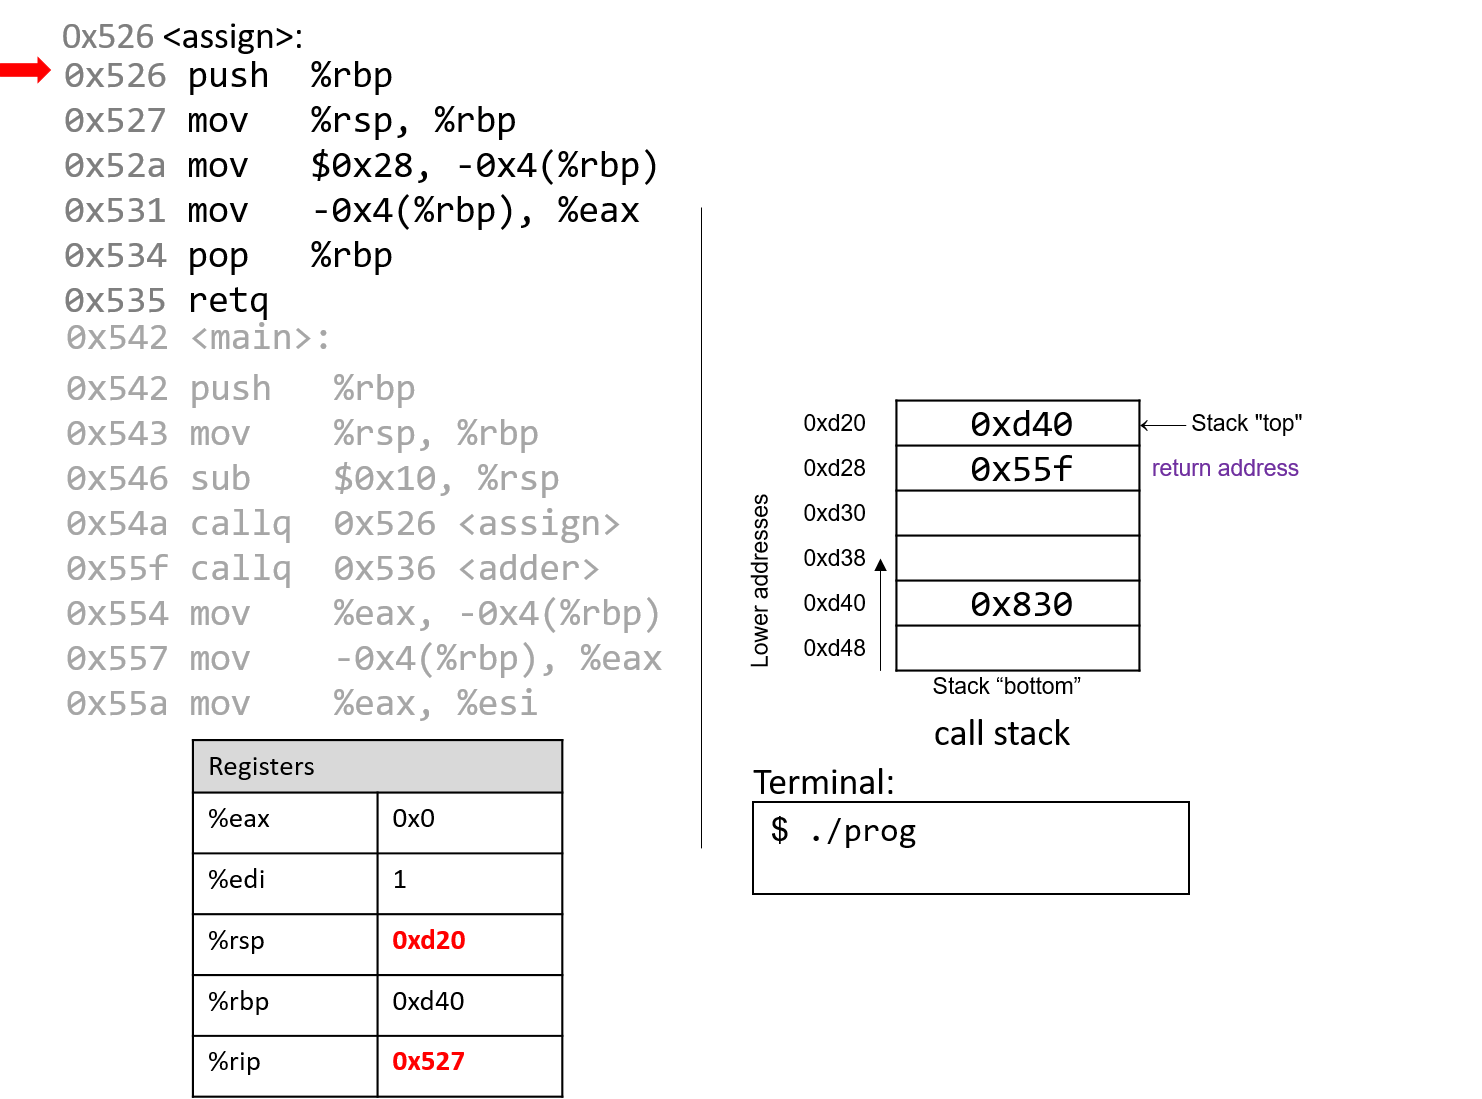
\includegraphics[scale=0.5]{img/Slide6.png}
            \end{center}

          \item \texttt{\%rip} is incremented to the next address. We then update the base pointer to the top of the stack. 
            \begin{center}
              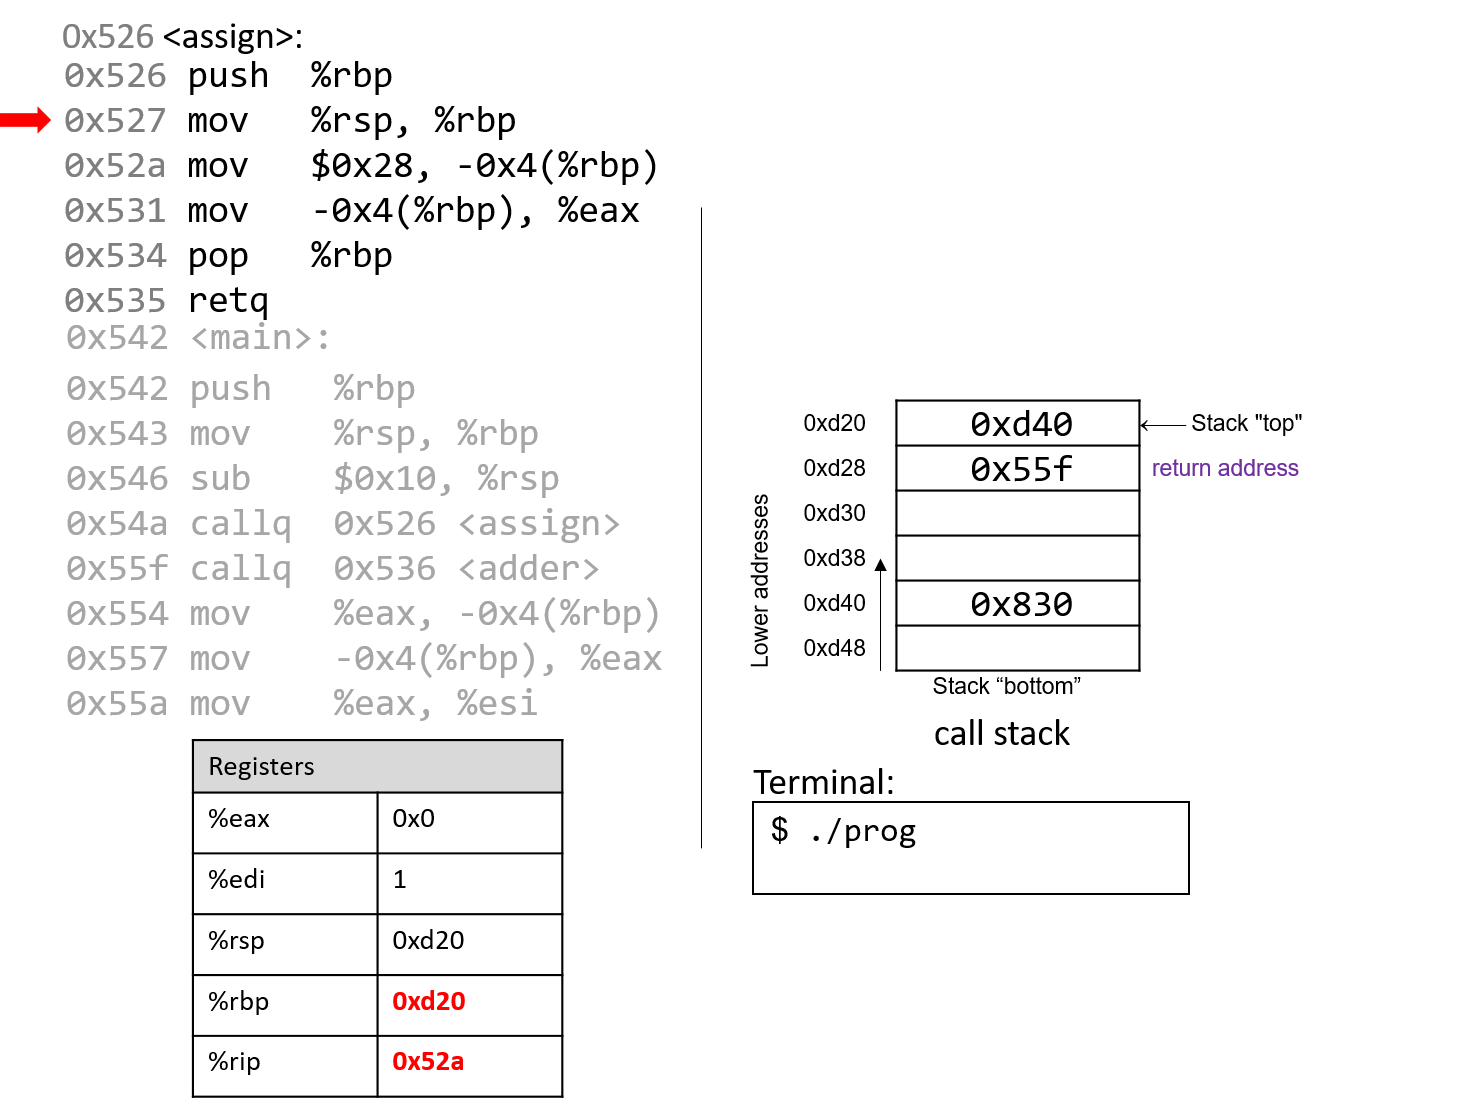
\includegraphics[scale=0.5]{img/Slide7.png}
            \end{center}

          \item Now we want to move the number \texttt{0x28} (40) into the memory location \texttt{-0x4(\%rbp)} of the stack, which is 4 bytes above the frame pointer, which is also the stack pointer. It is common that the frame pointer is used to reference locations on the stack. Note that this does not update the stack pointer.  
            \begin{center}
              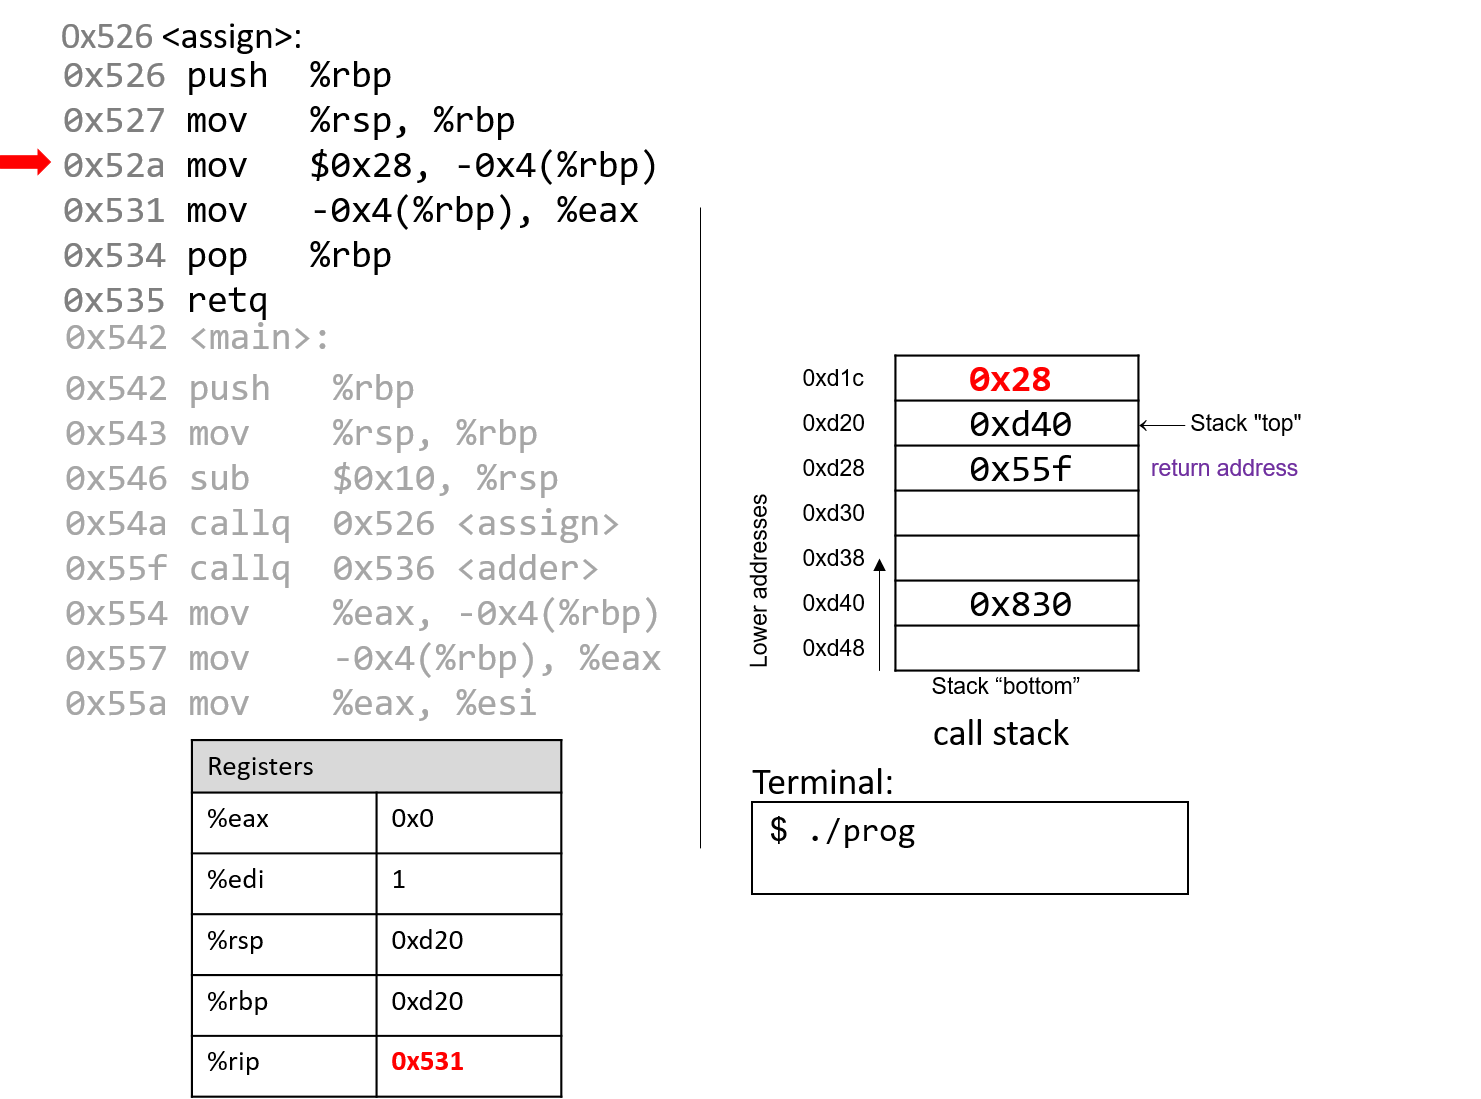
\includegraphics[scale=0.5]{img/Slide8.png}
            \end{center}

          \item Now we take the same address where we stored \texttt{0x28} to and move it into \texttt{\%eax}, effectively loading 40 onto the return value. 
            \begin{center}
              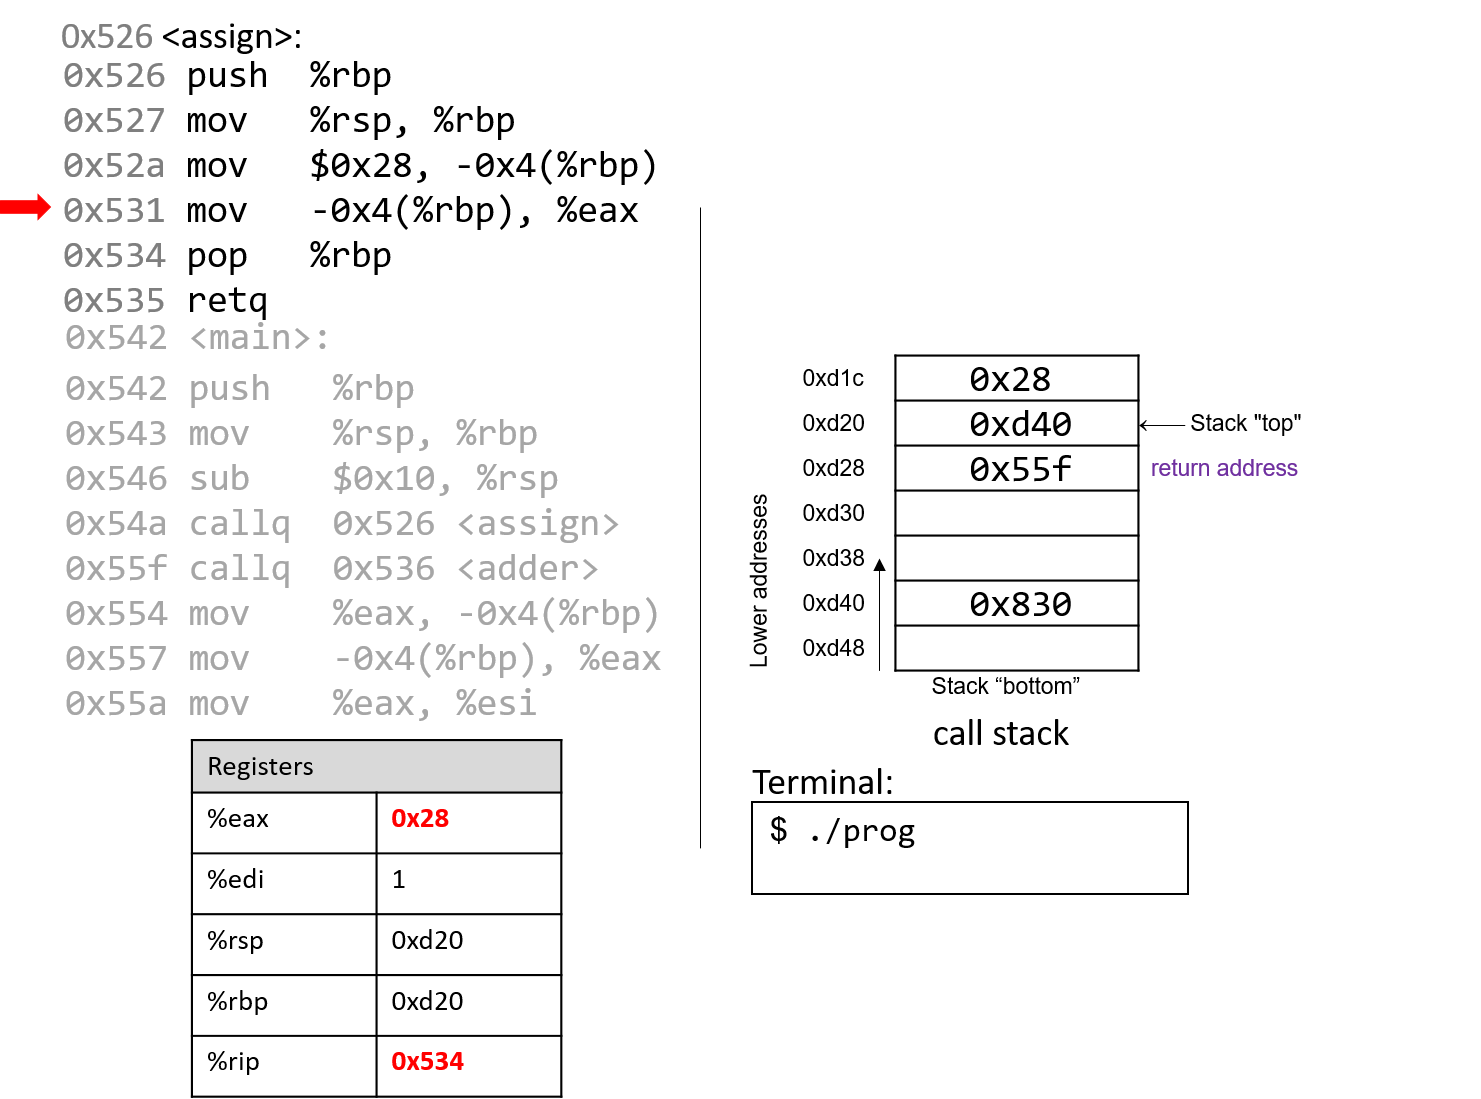
\includegraphics[scale=0.5]{img/Slide9.png}
            \end{center}

          \item We see that we will return this value soon, but before we do, we want to make sure that when the assign stack frame gets deleted (not really, but overwritten), we want to restore the base pointer of the main stack frame. We have already saved this before at \texttt{\%rsp}, which hasn't changed since we only worked with displacements from the base pointer. We retrieve the main stack pointer data and load it back into \texttt{\%rbp}. Note that this increments \texttt{\%rsp} by 8 bytes, shrinking the stack, and we are technically out of the assign stack frame. 
            \begin{center}
              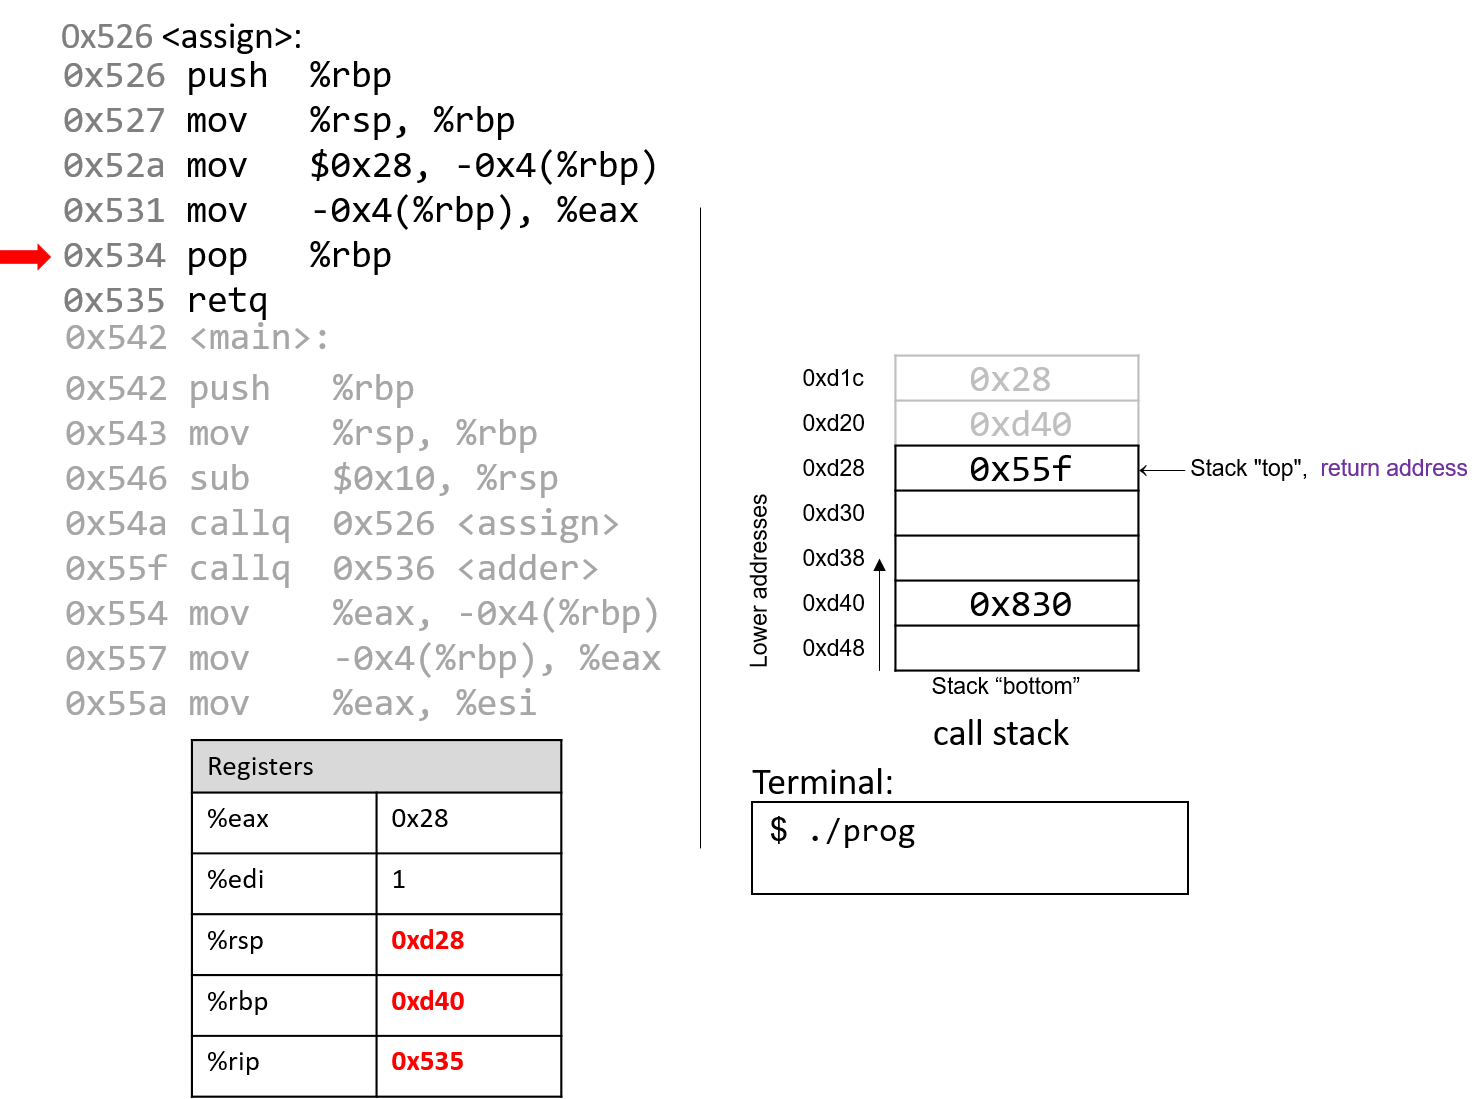
\includegraphics[scale=0.5]{img/Slide10.png}
            \end{center} 

          \item Note that at this point, since \texttt{\%rbp} was popped off, the next value that is at the top of the stack is the address \texttt{\%rip} that we store earlier, which points to the next execution in main. When \texttt{retq} executes, this value at the top of the stack is popped into \texttt{\%rip}, allowing main to continue executing within the main stack frame. Note that the return value is stored in \texttt{\%eax}.
            \begin{center}
              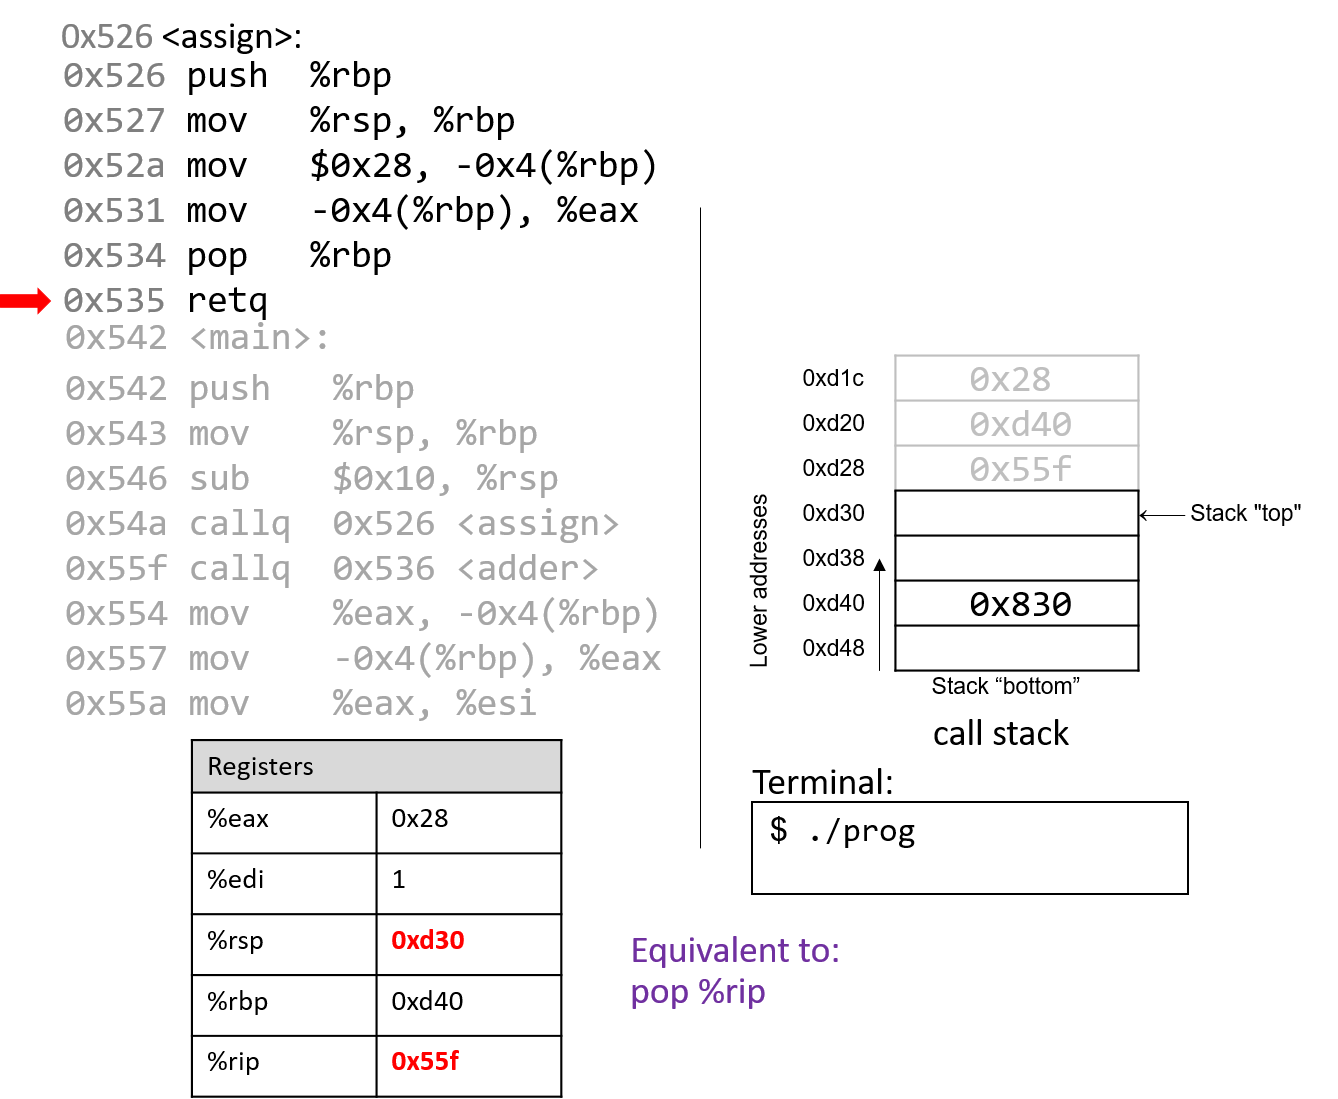
\includegraphics[scale=0.5]{img/Slide11.png}
            \end{center}

          \item Now we execute the next instruction in \texttt{\%rip} which is a call to the \texttt{adder} function. \texttt{\%rip} is automatically updated to the next address at \texttt{0x554}, but since this is a \texttt{callq} instruction, we first want to store this \texttt{\%rip} into the stack so we can come back to it, and then update \texttt{\%rip} to the first instruction in \texttt{adder}, which is address \texttt{0x536}. 
            \begin{center}
              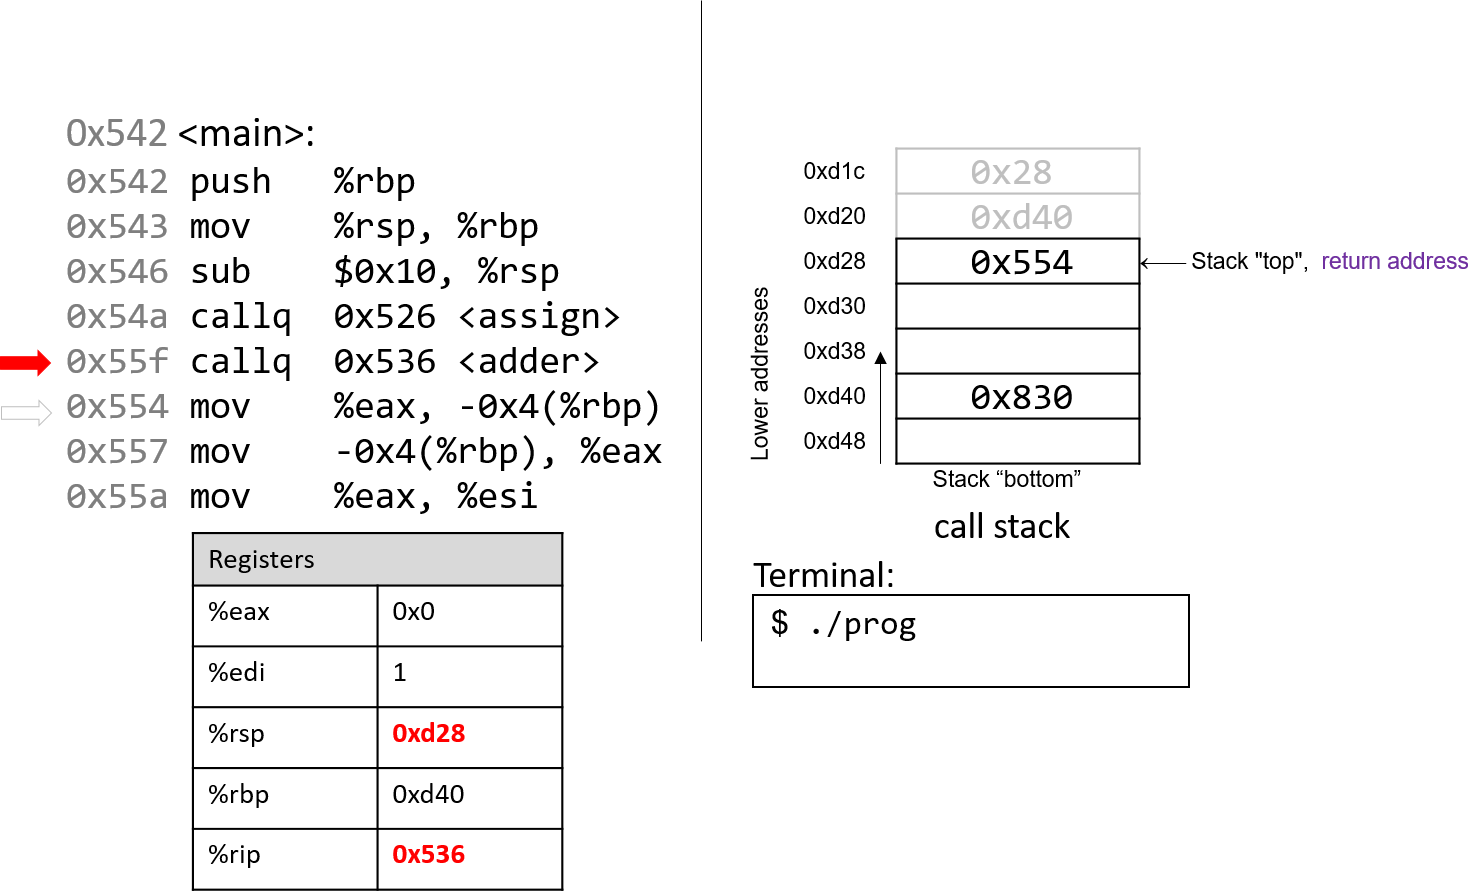
\includegraphics[scale=0.5]{img/Slide12.png}
            \end{center}

          \item Since we are in the adder function, this creates a new stack frame and we must update \texttt{\%rbp}. Again, we don't want to overwrite the base pointer of main, so we save it onto the stack by pushing \texttt{\%rbp}. 
            \begin{center}
              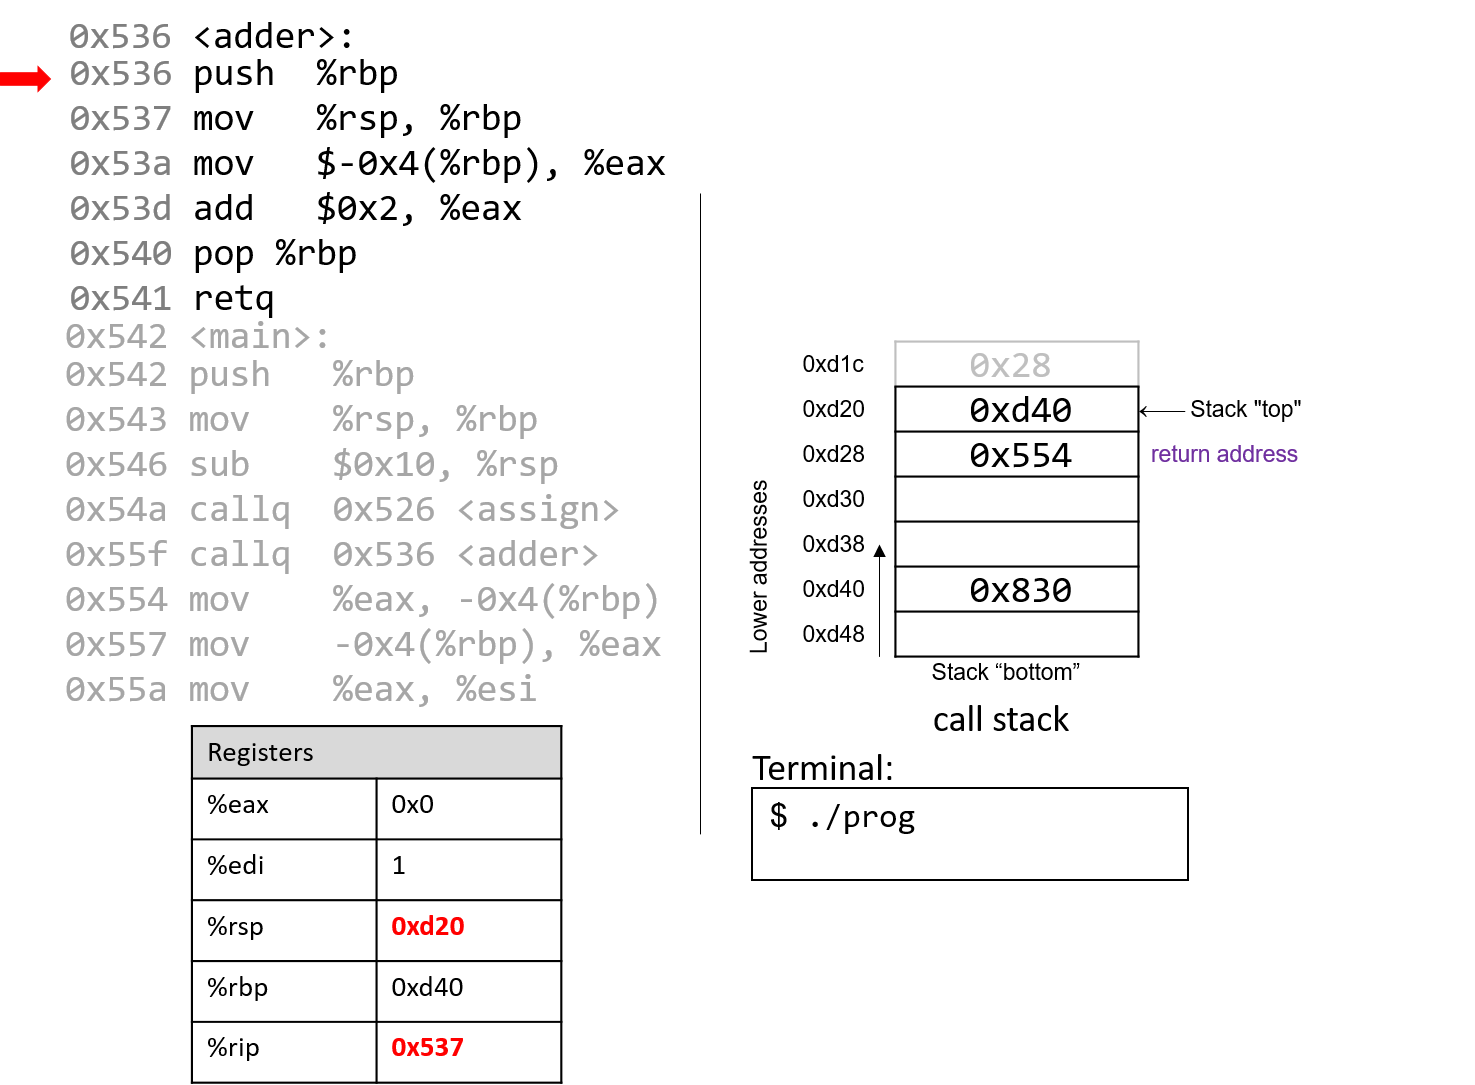
\includegraphics[scale=0.5]{img/Slide13.png}
            \end{center}

          \item Then we update \texttt{\%rbp} to the current stack pointer. 
            \begin{center}
              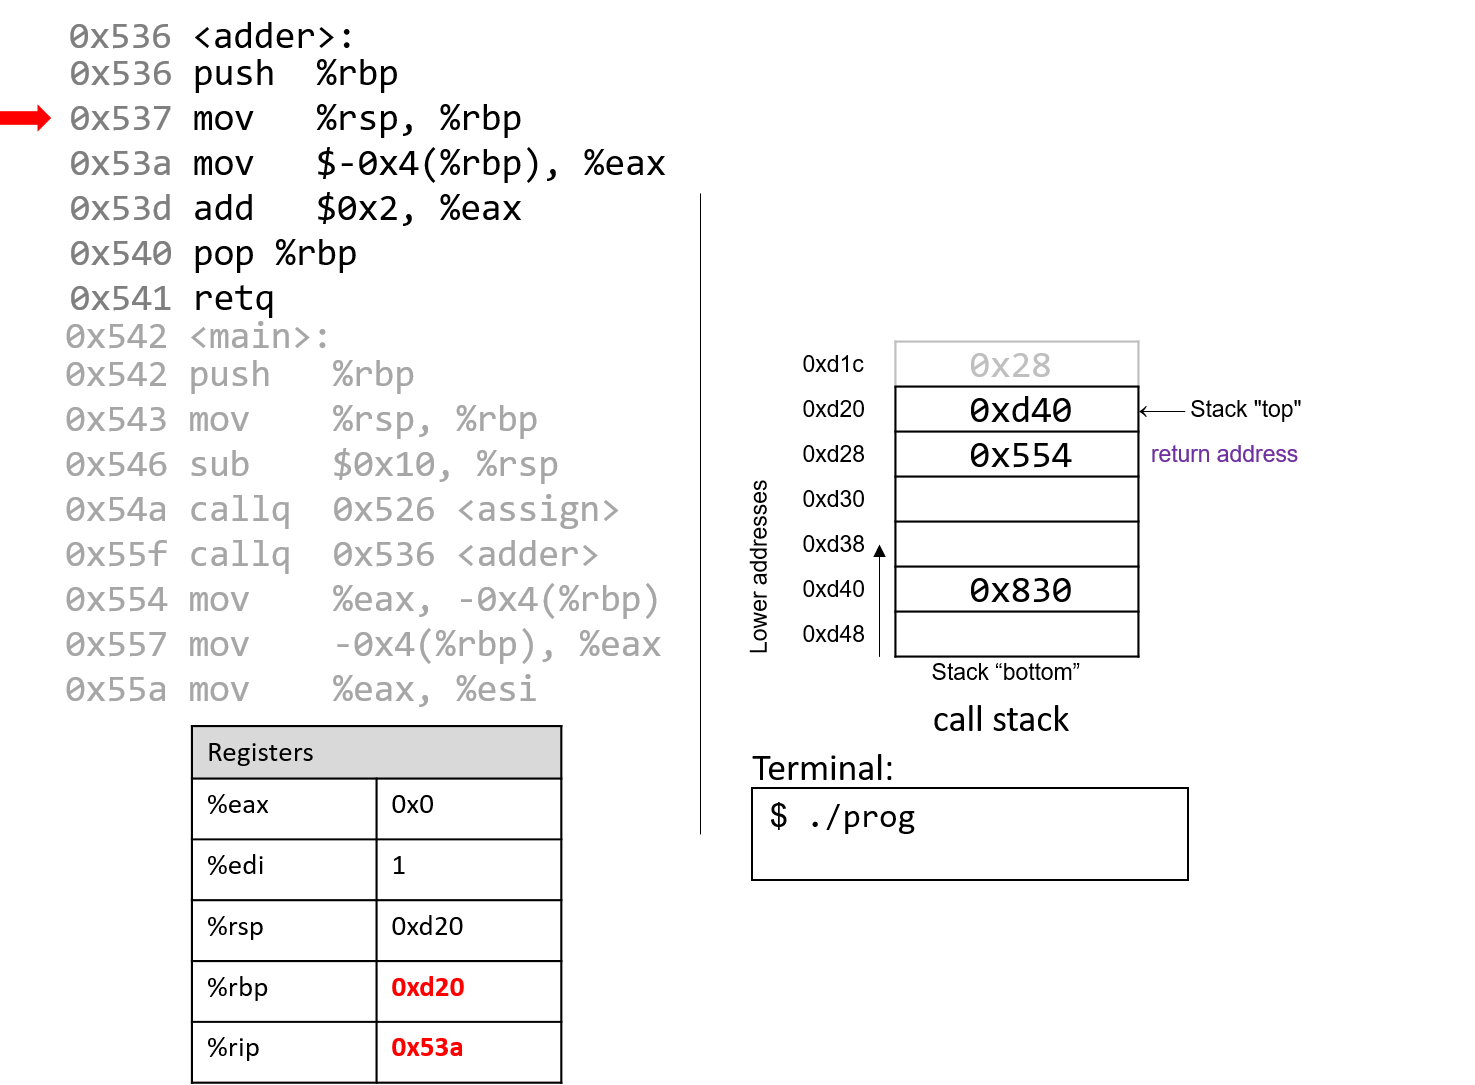
\includegraphics[scale=0.5]{img/Slide14.png}
            \end{center}

          \item This part is a bit tricky. Note that the value of \texttt{0x28} still lives at \texttt{0xd1c}, which is conveniently at address \texttt{-0x4(\%rbp)}. Therefore, when we call \texttt{int a;} in that corresponding line in \texttt{adder}, we can actually add 2 to it, though it seems like there was no value assigned to it. This is just a trick though. So, we can take these remnant value and store it into \texttt{\%eax}. 
            \begin{center}
              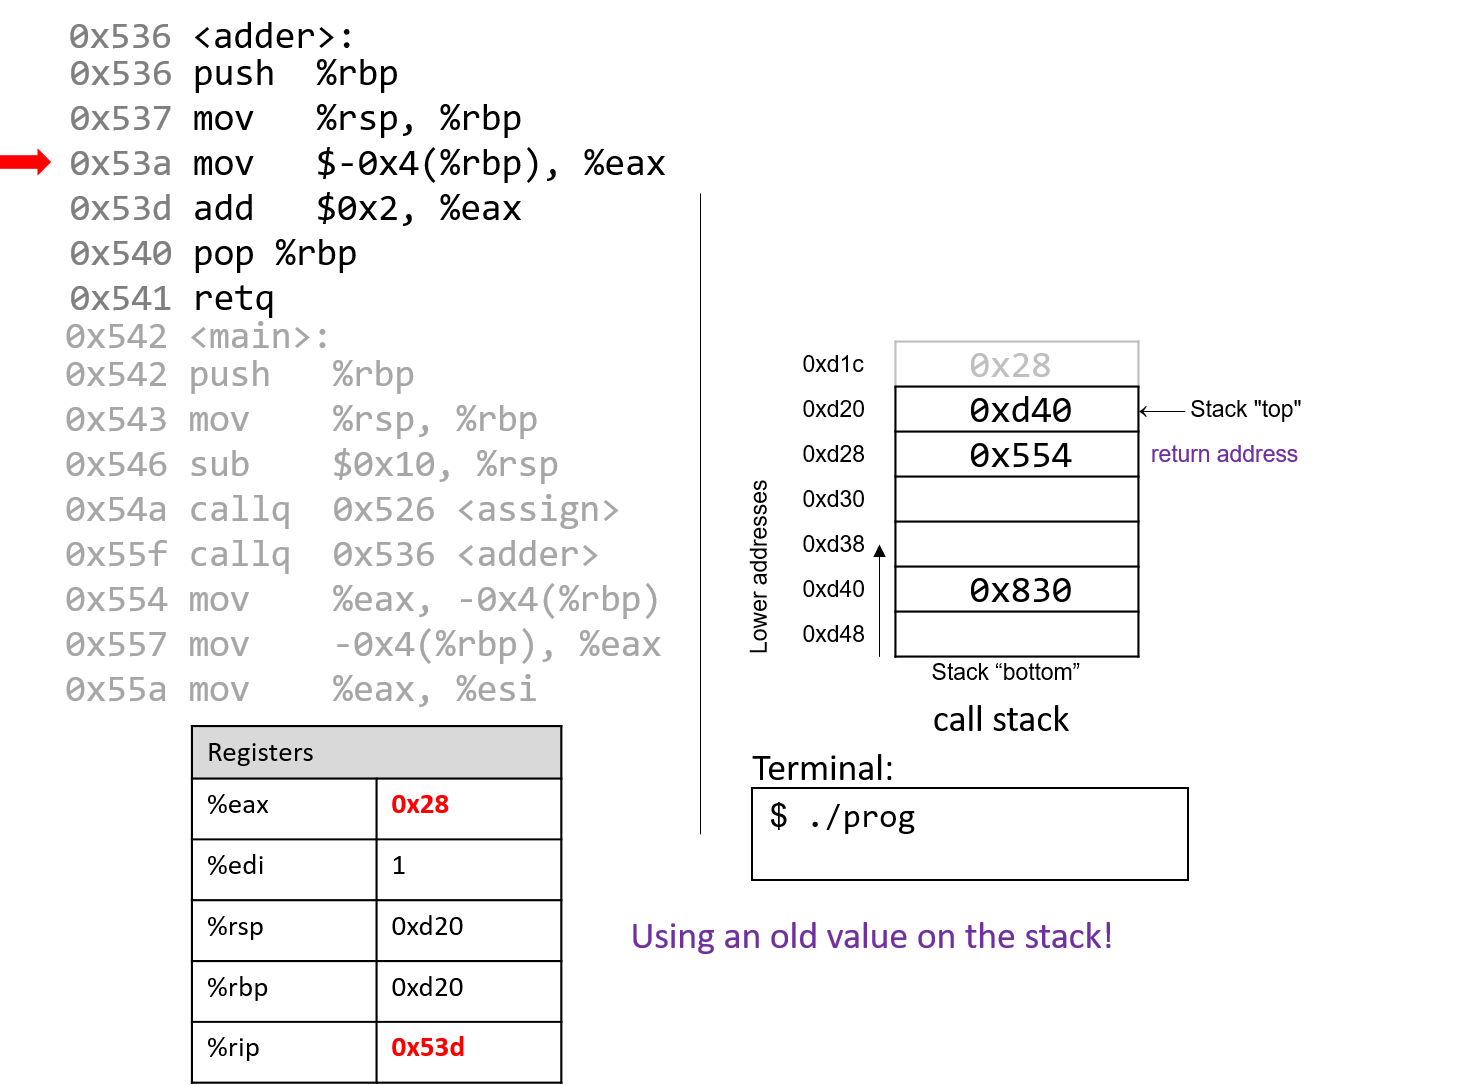
\includegraphics[scale=0.5]{img/Slide15.png}
            \end{center}

          \item We then add 2 to it. 
            \begin{center}
              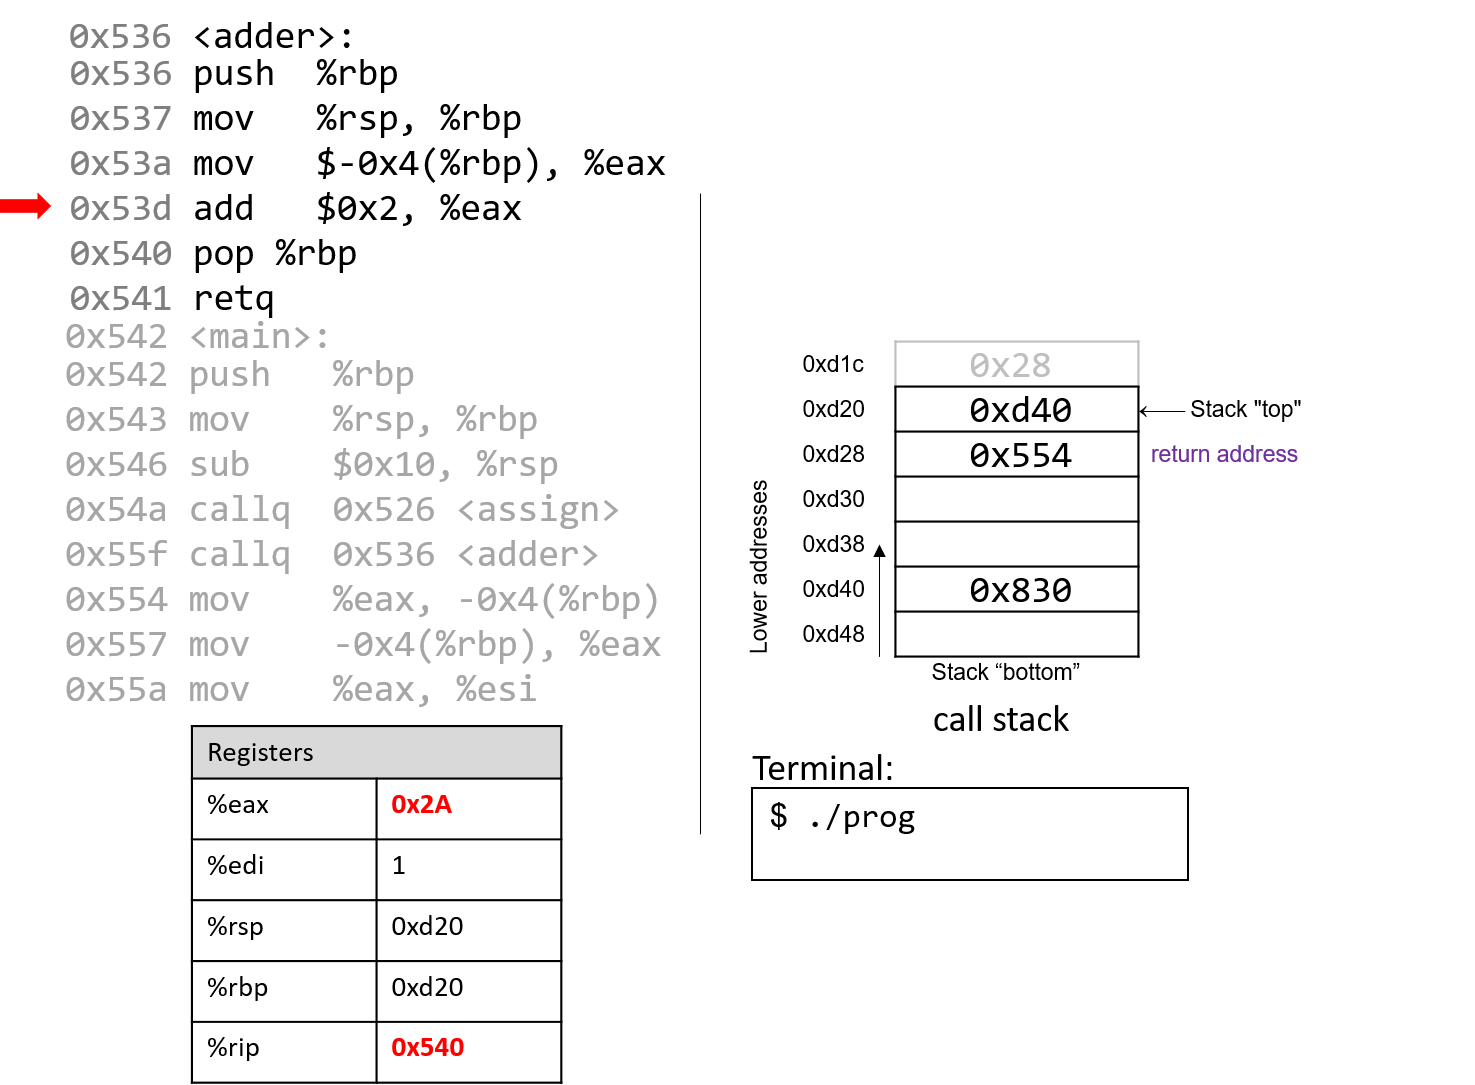
\includegraphics[scale=0.5]{img/Slide16.png}
            \end{center}

          \item Now we are almost done, so we pop the base pointer of the main stack frame, at \texttt{0xd40}, back into \texttt{\%rbp}. 
            \begin{center}
              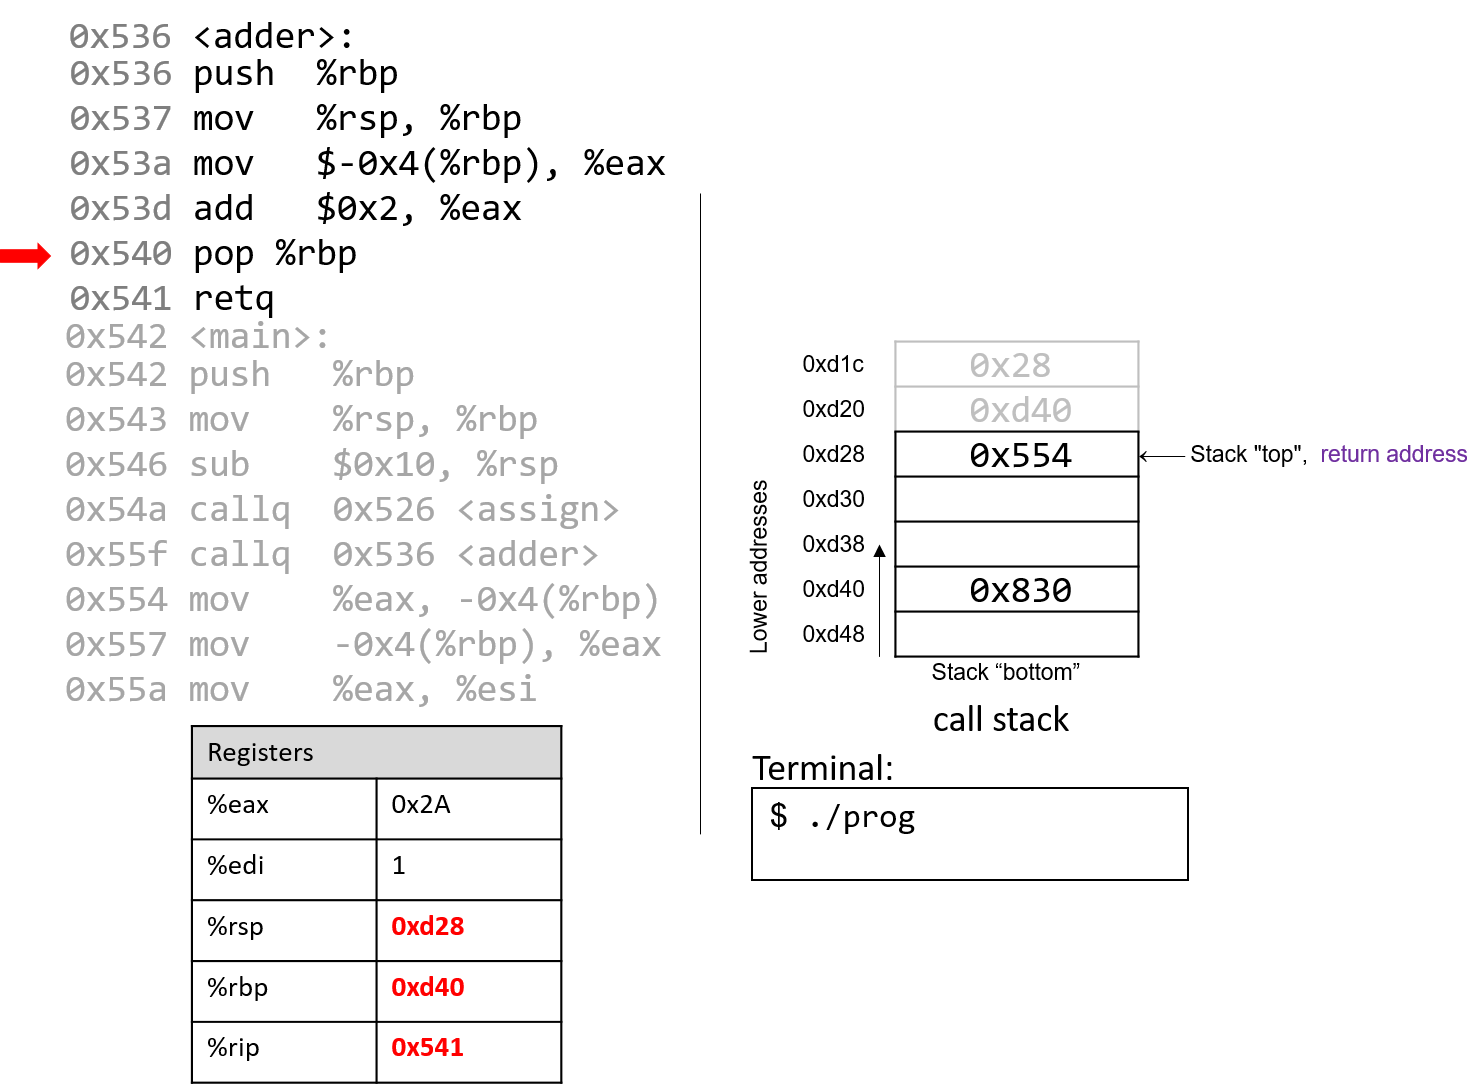
\includegraphics[scale=0.5]{img/Slide17.png}
            \end{center}

          \item We now return the value in \texttt{\%eax} and pop the base pointer of the adder stack frame, which simply updates the instruction pointer \texttt{\%rip} back to the next instruction in main. This is equivalent to \texttt{pop \%rip}, which is equivalent to moving the stack pointer \texttt{\%rsp} into \texttt{\%rip} and then shrinking the stack by 8 bytes \texttt{subq \$8, \%rsp}. 
            \begin{center}
              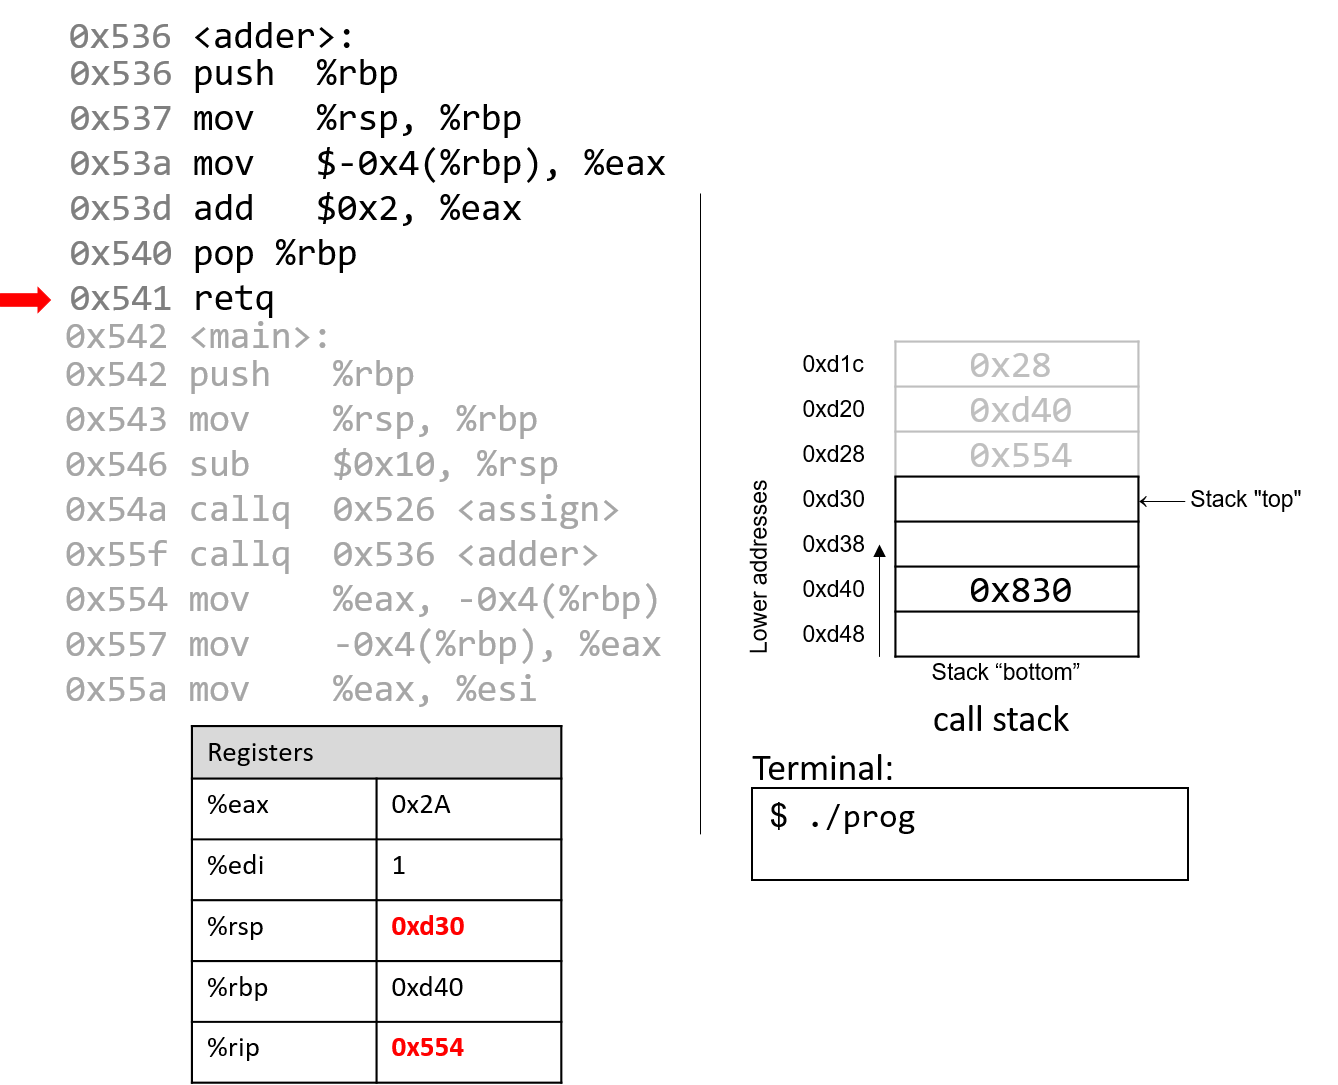
\includegraphics[scale=0.5]{img/Slide18.png}
            \end{center}

          \item Now it is relatively straightforward since we do the rest in main (except for the print statement). The current value in \texttt{\%eax} represents the return value of adder. We want to put this in the variable \texttt{x}, which we have already allocated some memory for right above the base pointer in the main stack frame. We move it there. Note that right after, it places this right back into \texttt{\%eax}.
            \begin{center}
              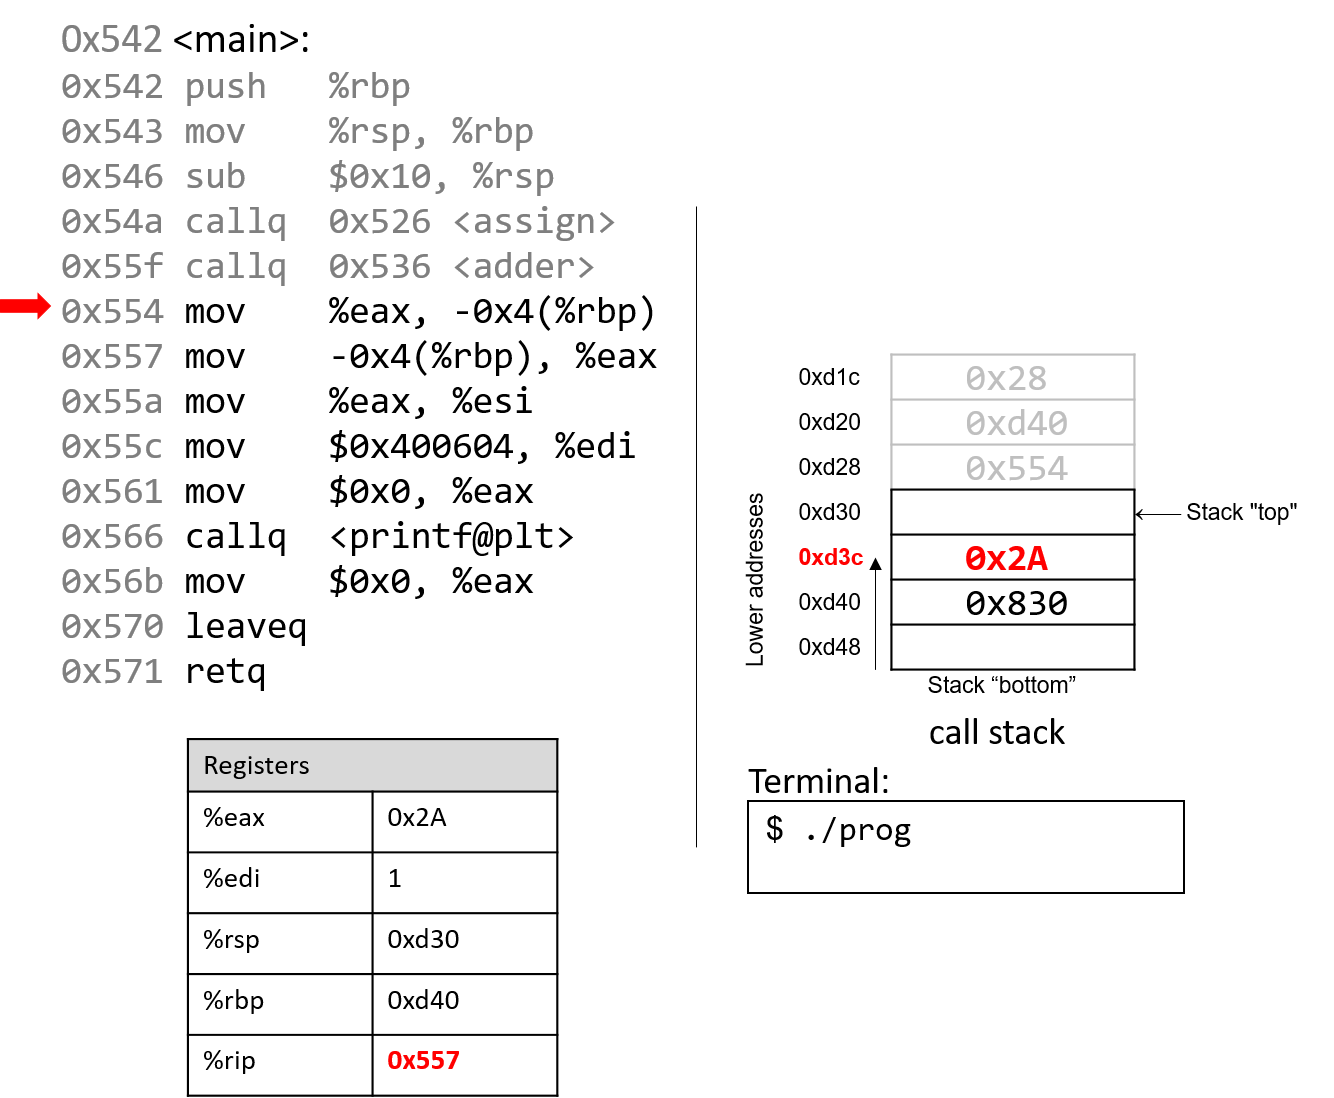
\includegraphics[scale=0.5]{img/Slide19.png}
            \end{center}

          \item the mov instruction at address 0x55a copies the value in \texttt{\%eax} (or 0x2A) to register \texttt{\%esi}, which is the 32-bit component register associated with \texttt{\%rsi} and typically stores the second parameter to a function. We can see why since this will be put into a print statement, which is a function, and \texttt{x = \%esi} is the second argument of \texttt{printf}. 
            \begin{center}
              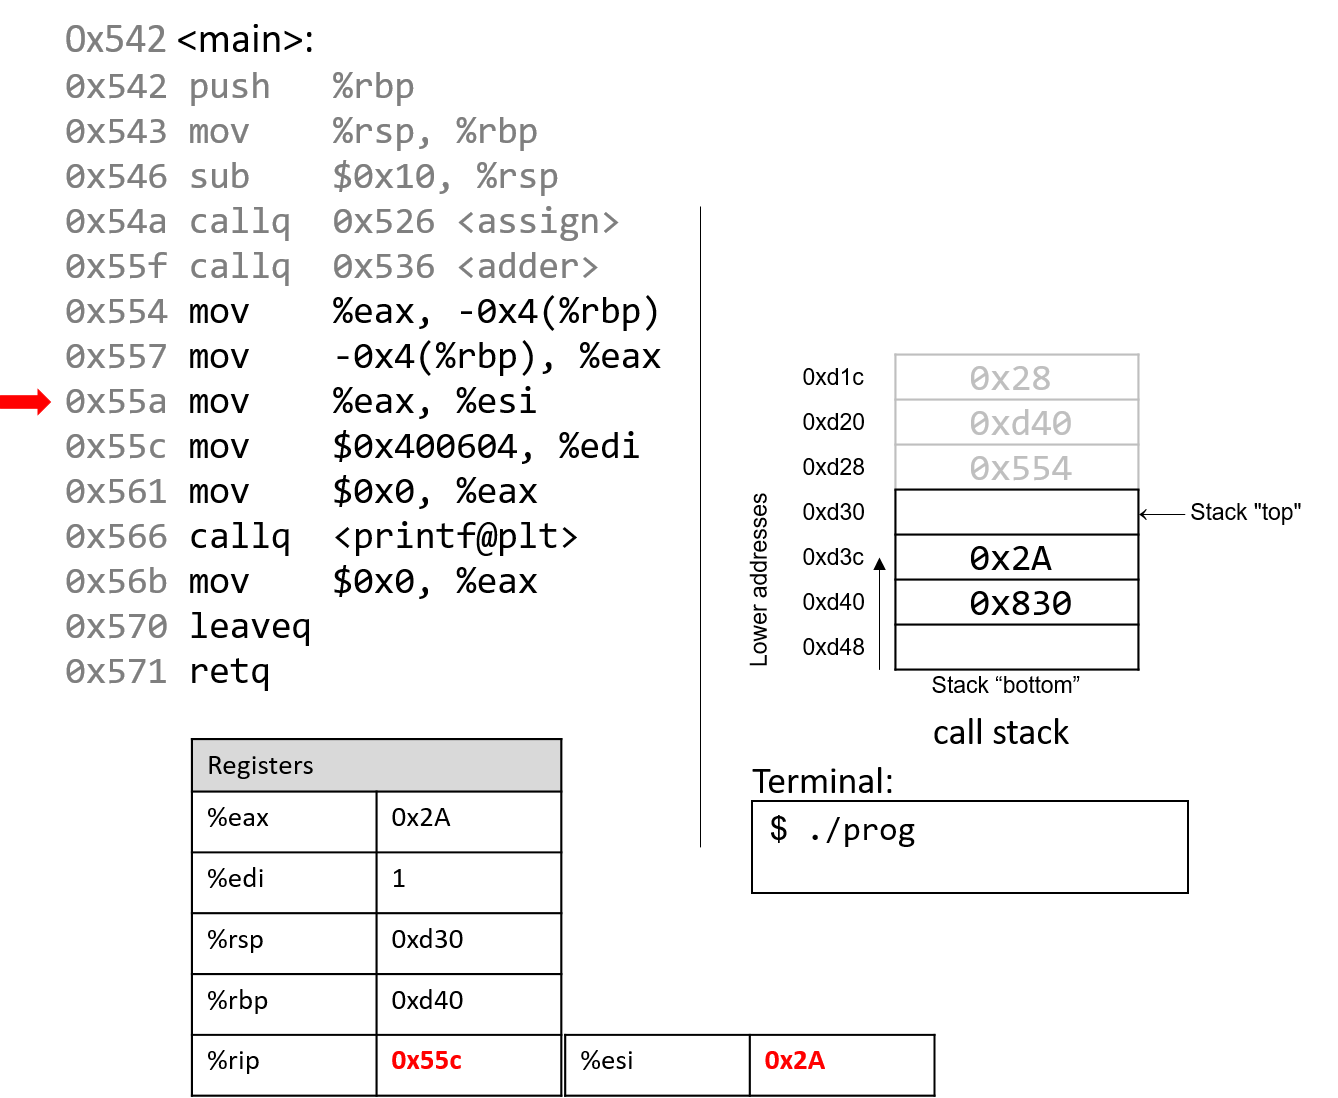
\includegraphics[scale=0.5]{img/Slide21.png}
            \end{center}

          \item Now we want to retrieve the first argument of the print function. The address at \texttt{\$0x400604} is some address in the code segment memory that holds the string \texttt{"x is \%d\textbackslash n"}. 
            \begin{center}
              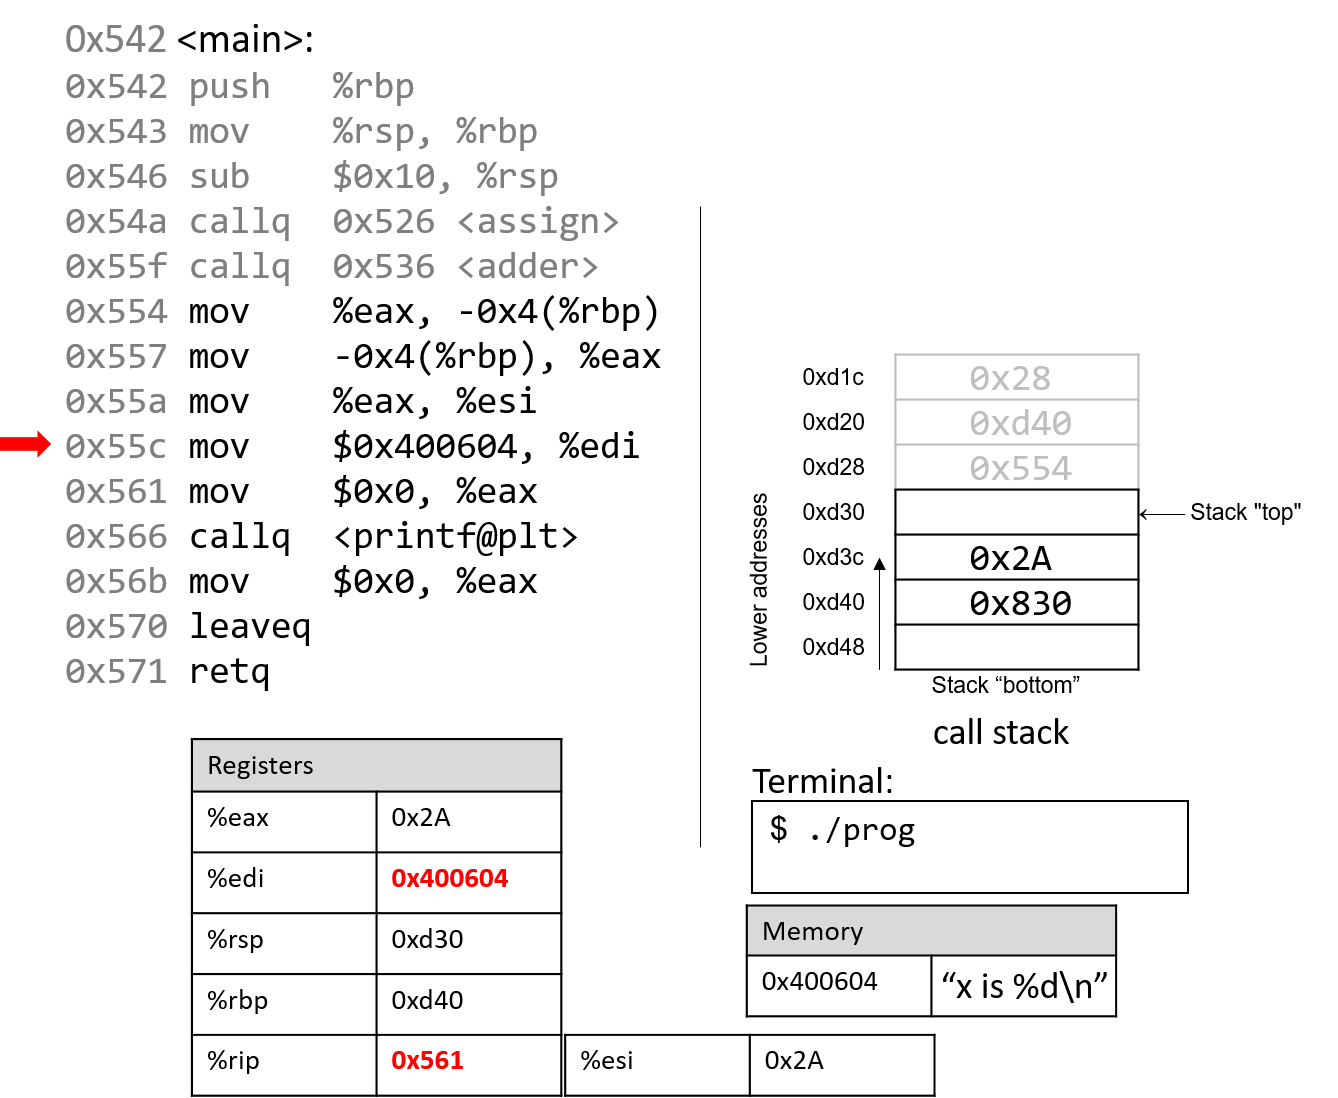
\includegraphics[scale=0.5]{img/Slide22.png}
            \end{center}

          \item Then we move $0$ into the \texttt{\%eax} register to clear it. 
            \begin{center}
              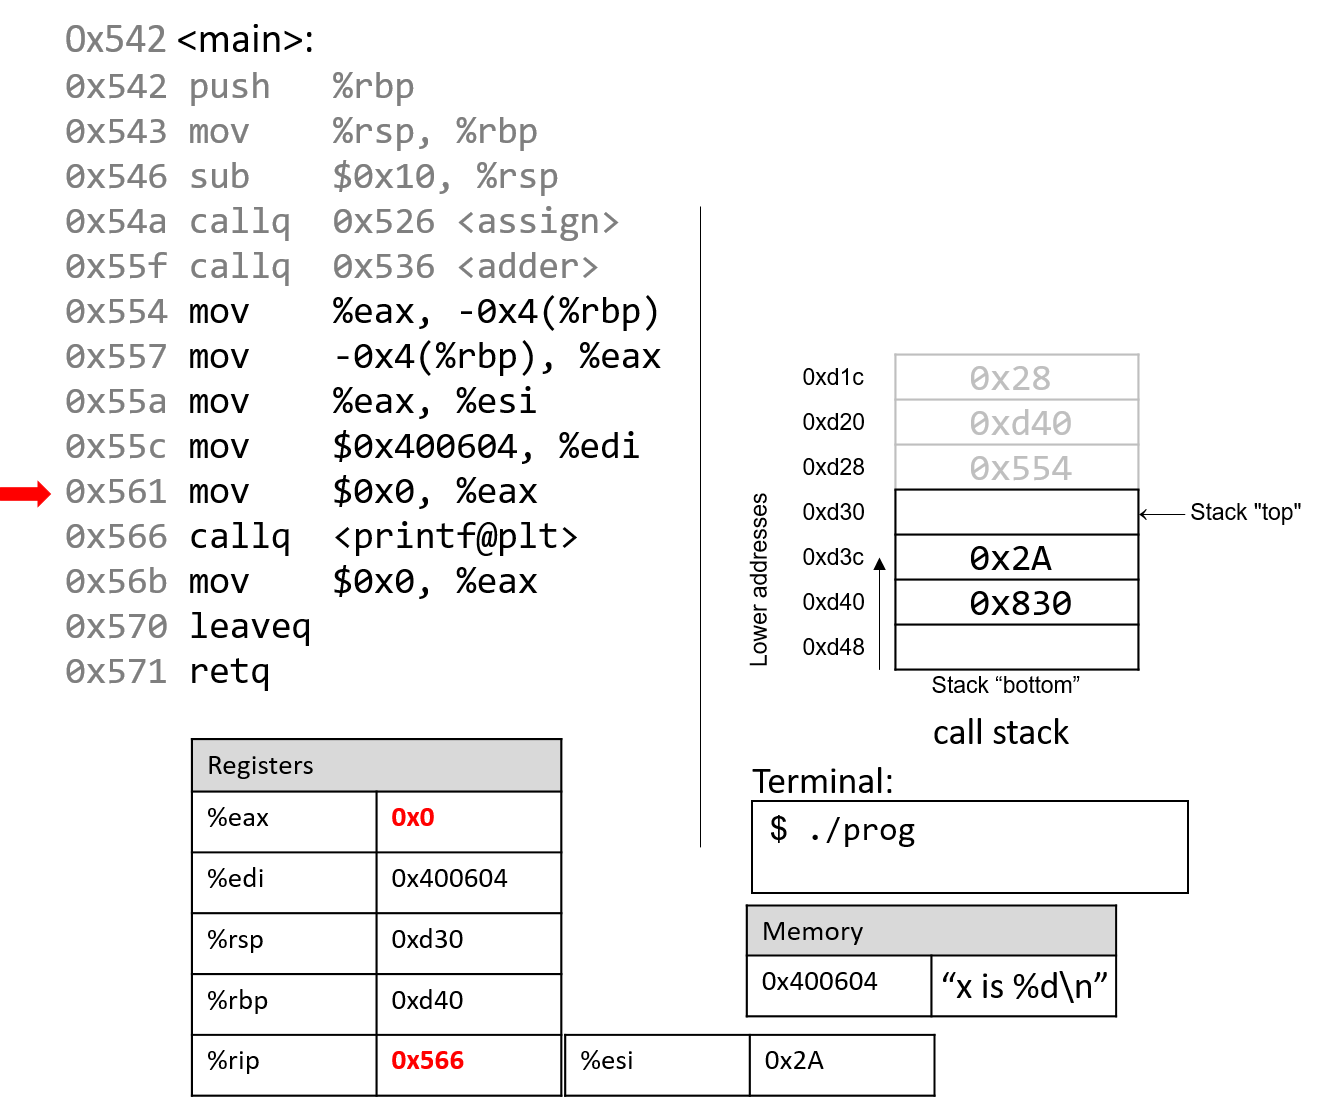
\includegraphics[scale=0.5]{img/Slide23.png}
            \end{center} 

          \item We then call the \texttt{printf} function, which we won't trace through but it outputs to stdout.  
            \begin{center}
              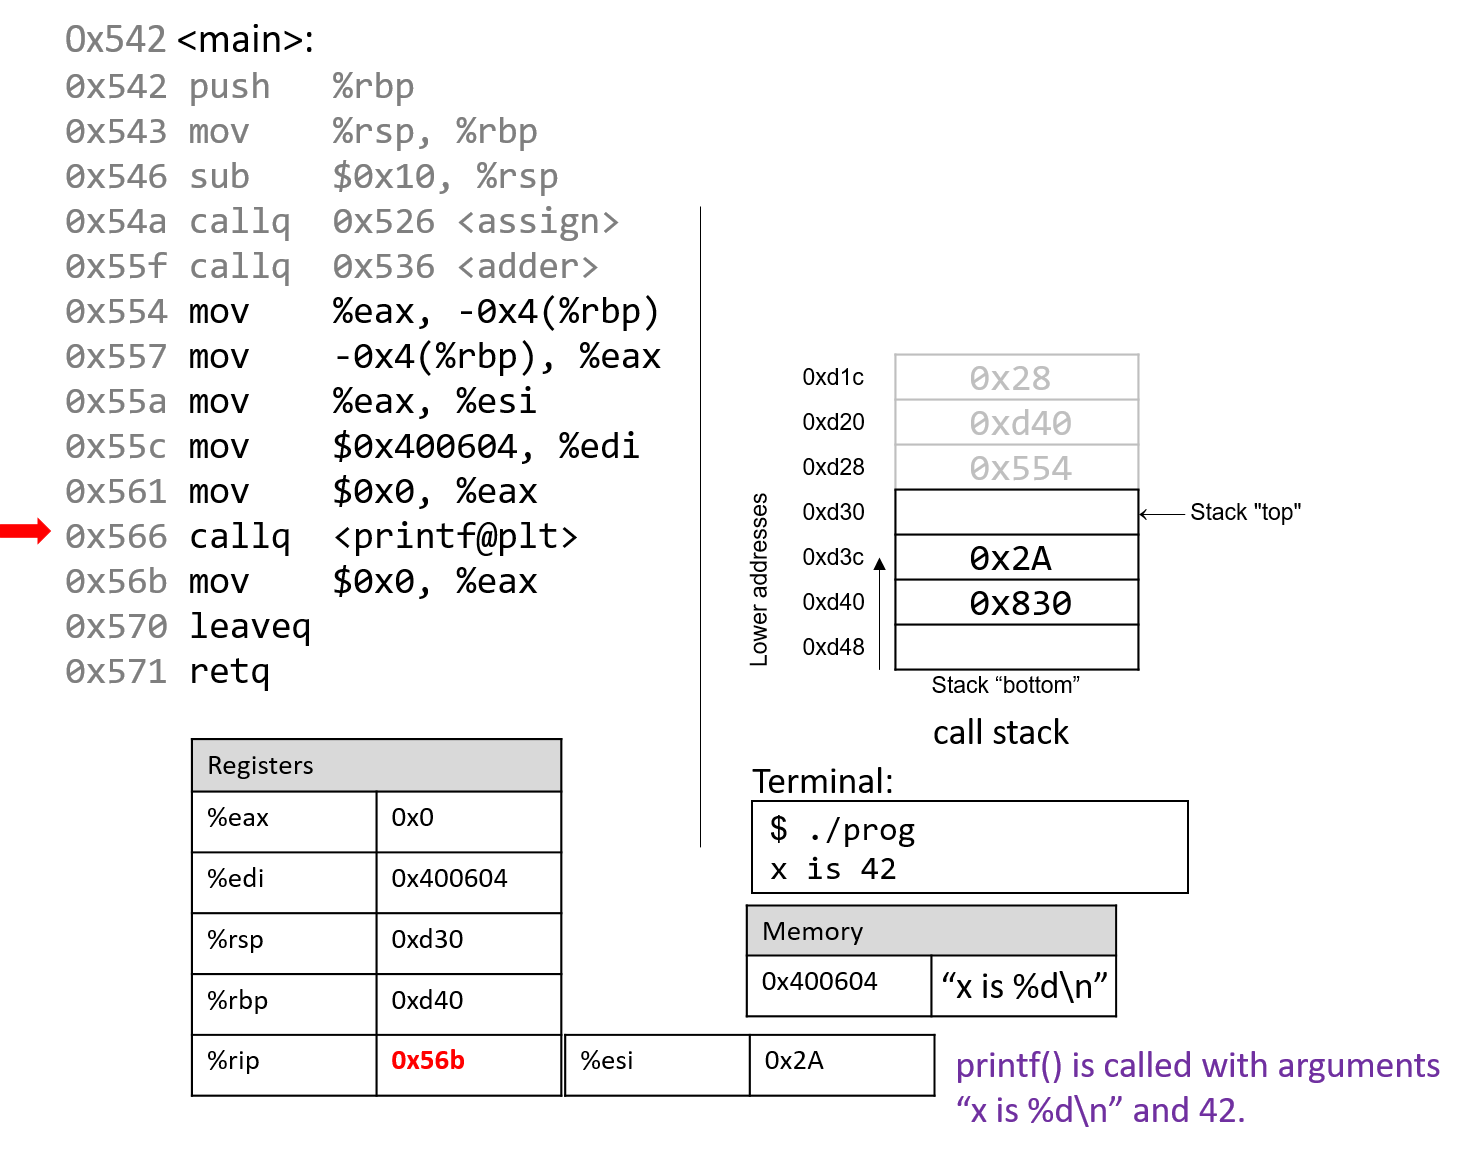
\includegraphics[scale=0.5]{img/Slide24.png}
            \end{center}

          \item The print function might have returned something, but we don't care. We want to main function to return 0, so we move 0 into \texttt{\%eax}. 
            \begin{center}
              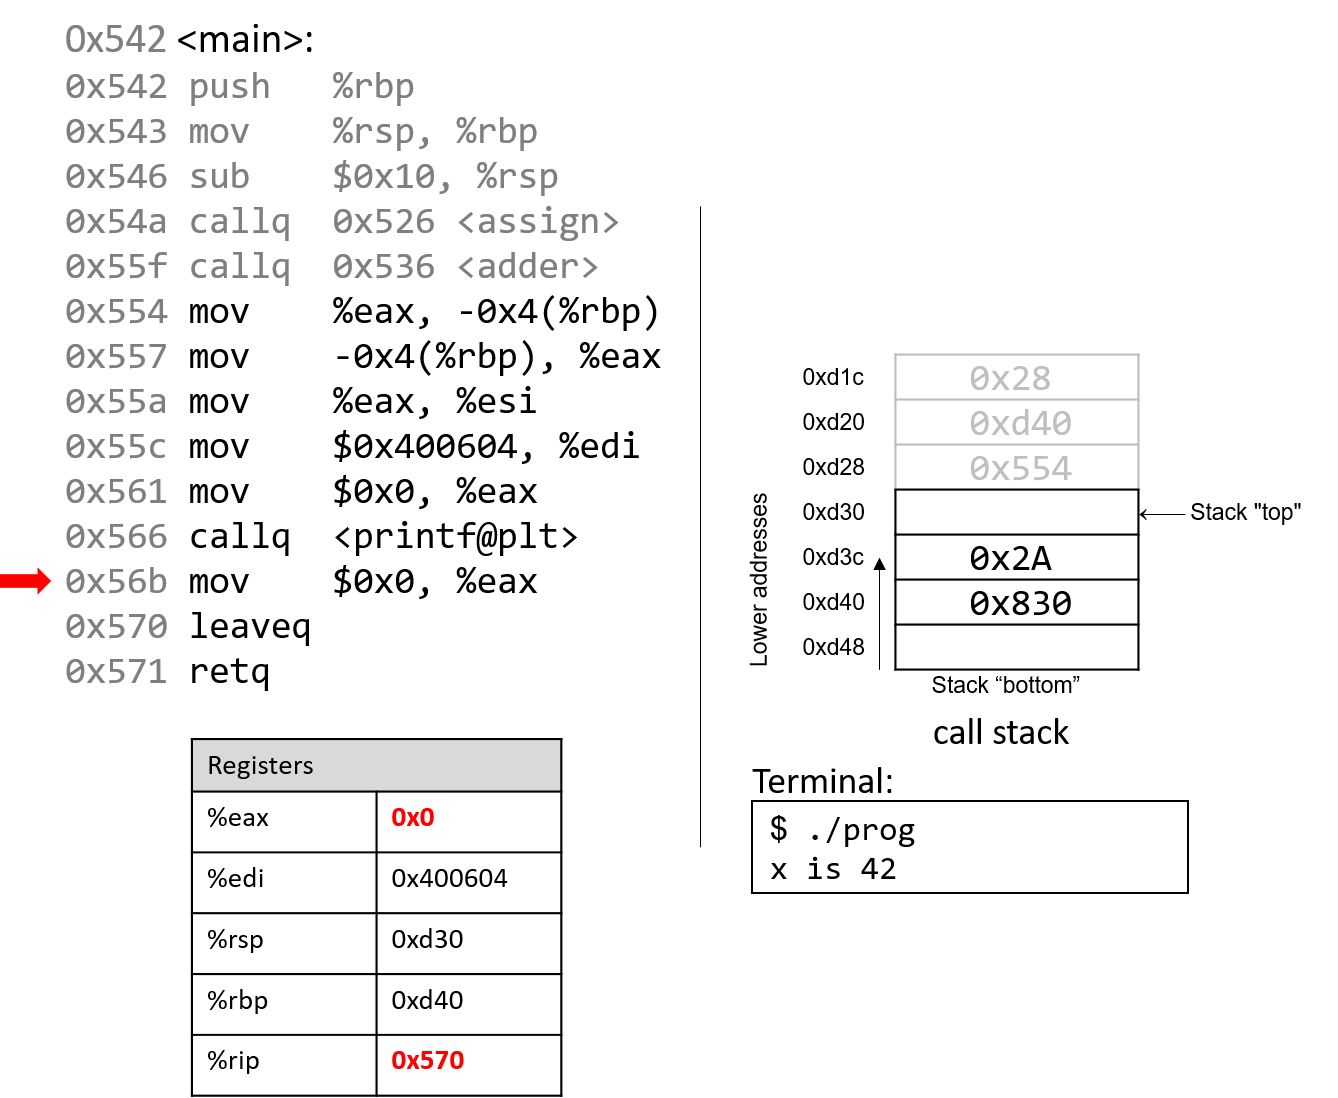
\includegraphics[scale=0.5]{img/Slide25.png}
            \end{center}

          \item Finally we execute \texttt{leaveq}, which prepares the stack for returning from the function call. It essentially moves the base pointer back to the stack pointer and then pops the base pointer off the stack. The new \texttt{\%rbp} is the original base pointer of whatever was outside the main function, \texttt{0x830}. 
            \begin{center}
              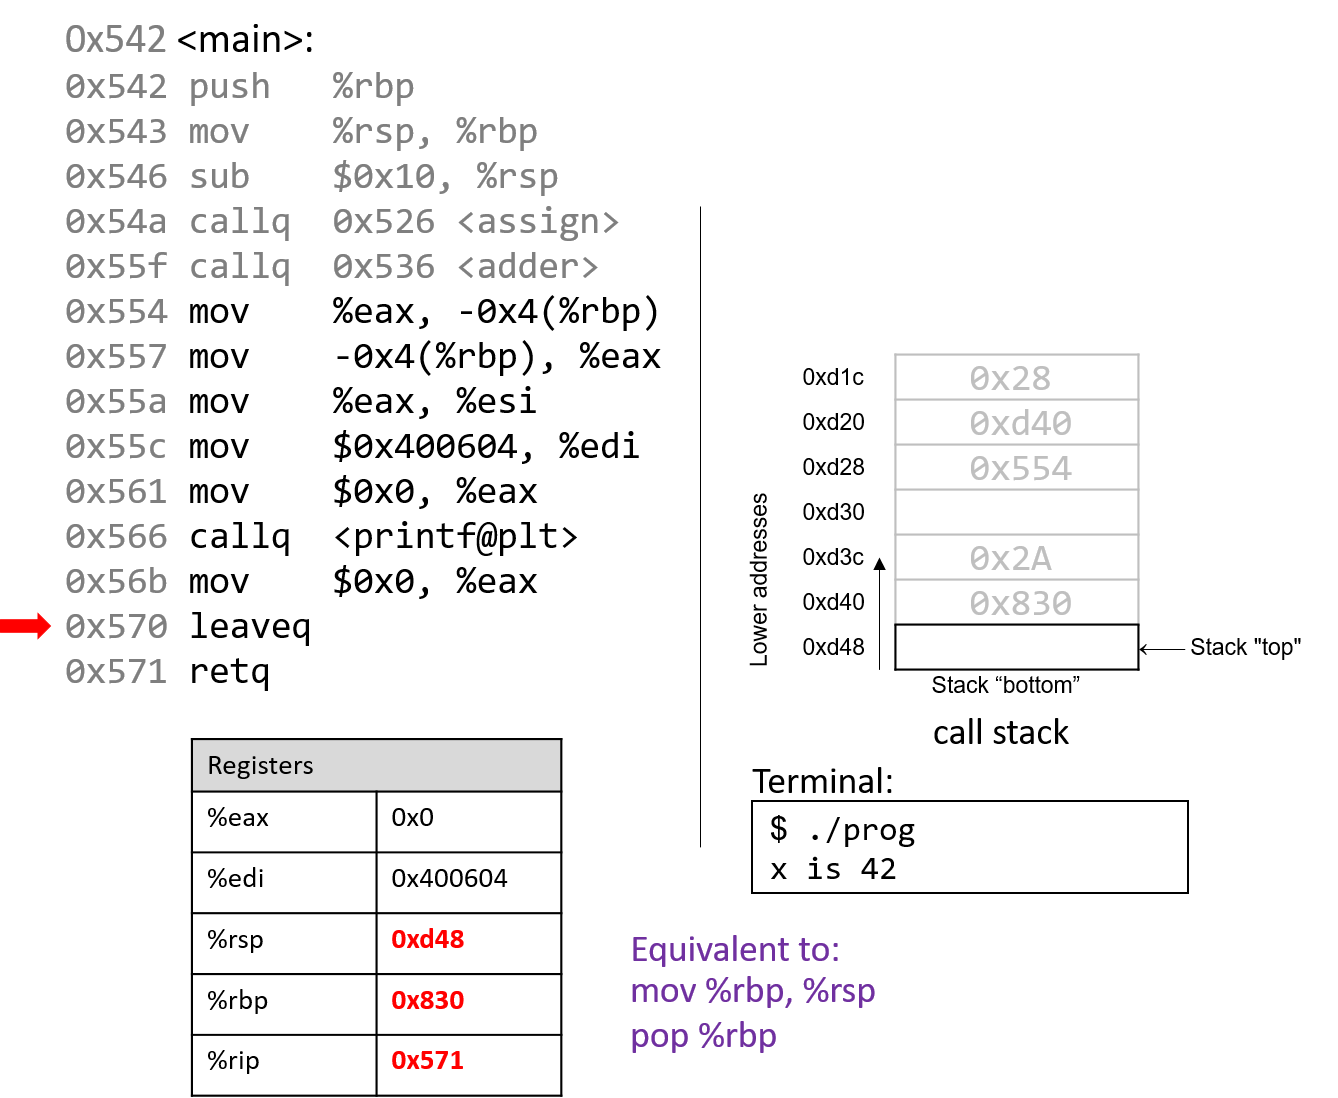
\includegraphics[scale=0.5]{img/Slide26.png}
            \end{center}

          \item Finally, we execute \texttt{retq}, which pops the return address off the stack and puts it into \texttt{\%rip}. 
        \end{enumerate}
      \end{example}

      There is a bit of a concern here from the previous example. The main function had two functions that returned two values. As the subfunction stack frame is removed from the stack, the return value is stored in the \texttt{\%rax} register. If another function is called right after, then the return value of the second function will overwrite that of the previous one. This was not a problem in the previous example since the return value of the \texttt{assign} function was not used. However, if it was, then the return value of the \texttt{adder} function would have overwritten it. This is known as register saving. 
      \begin{enumerate}
        \item For \textbf{caller-saved registers}, the caller function is responsible for saving the value of the register before calling a function and restoring it after the function returns. The caller should save values in its stack frame before calling the callee function, e.g. by pushing all the return values of each callee in the caller stack frame. Then it will restore values after the call. 

        \begin{center}
          \textit{Therefore, if we have a set of registers $\{\texttt{\%reg}\}$, the caller must take everything and push them in the caller stack frame. Then it will restore them after the call.}
        \end{center}

        \item For \textbf{callee-saved registers}, it is the callee's repsonsibility to save any data in these registers before using the registers. 

          \begin{center} 
            \textit{Therefore, if we have a set of registers $\{\texttt{\%reg}\}$, then inside the callee stack frame, the callee must take everything and push them in the callee stack frame. Once it computes the final return value, then it will restore all the saved register values from the callee stack frame back into the registers for the caller to use.}
          \end{center}
      \end{enumerate}

      Ideally, we want \textit{one} calling convention to simply separate implementation details between caller and callee. In general, however, neither is best. If the caller isn't using a register, then caller-save is better, and if callee doesn't need a register, then callee-save is better. If we do need to save, then callee save generally makes smaller programs, so we compromise and use a combination of both caller-save and callee-save. The compiler tries to pick these registers, and by convention in x86, we have the following. 

      \begin{figure}[H]
        \centering 
        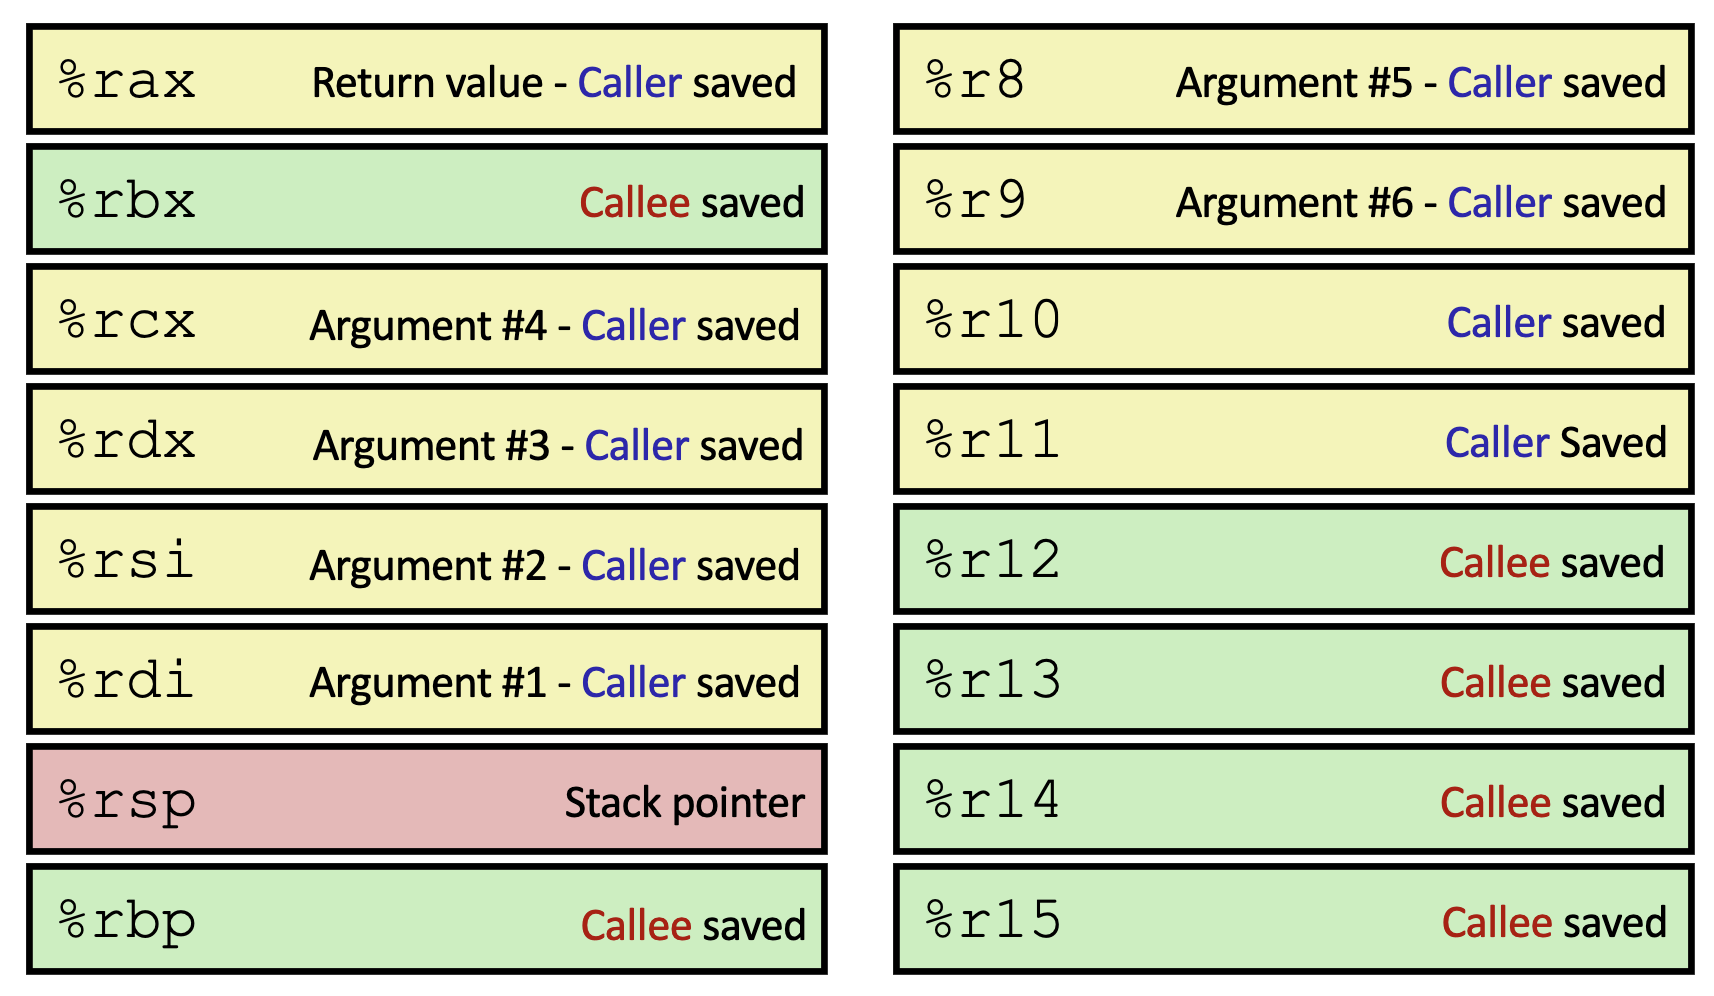
\includegraphics[scale=0.4]{img/caller_callee_save.png}
        \caption{Caller save and callee save registers. } 
        \label{fig:caller_callee_save}
      \end{figure}



    \subsubsection{Recursion} 

    \subsubsection{Arrays}

      For arrays, there's not anything new here. Let's go over some code and follow through it. 

      \begin{lstlisting}
        int sumArray(int *array, int length) {
          int i, total = 0;
          for (i = 0; i < length; i++) {
            total += array[i];
          }
          return total;
        }
      \end{lstlisting}

      This function takes the address of an array and the length of it and sums up all the elements in the array. 

      \begin{lstlisting}
        0x400686 <+0>:	push %rbp                   # save %rbp
        0x400687 <+1>:	mov  %rsp,%rbp              # update %rbp (new stack frame)
        0x40068a <+4>:	mov  %rdi,-0x18(%rbp)       # copy array to %rbp-0x18
        0x40068e <+8>:	mov  %esi,-0x1c(%rbp)       # copy length to %rbp-0x1c
        0x400691 <+11>:	movl $0x0,-0x4(%rbp)        # copy 0 to %rbp-0x4 (total)
        0x400698 <+18>:	movl $0x0,-0x8(%rbp)        # copy 0 to %rbp-0x8 (i)
        0x40069f <+25>:	jmp  0x4006be <sumArray+56> # goto <sumArray+56>
        0x4006a1 <+27>:	mov  -0x8(%rbp),%eax        # copy i to %eax
        0x4006a4 <+30>:	cltq                        # convert i to a 64-bit integer
        0x4006a6 <+32>:	lea  0x0(,%rax,4),%rdx      # copy i*4 to %rdx
        0x4006ae <+40>:	mov  -0x18(%rbp),%rax       # copy array to %rax
        0x4006b2 <+44>:	add  %rdx,%rax              # compute array+i*4, store in %rax
        0x4006b5 <+47>:	mov  (%rax),%eax            # copy array[i] to %eax
        0x4006b7 <+49>:	add  %eax,-0x4(%rbp)        # add %eax to total
        0x4006ba <+52>:	addl $0x1,-0x8(%rbp)        # add 1 to i (i+=1)
        0x4006be <+56>:	mov  -0x8(%rbp),%eax        # copy i to %eax
        0x4006c1 <+59>:	cmp  -0x1c(%rbp),%eax       # compare i to length
        0x4006c4 <+62>:	jl   0x4006a1 <sumArray+27> # if i<length goto <sumArray+27>
        0x4006c6 <+64>:	mov  -0x4(%rbp),%eax        # copy total to %eax
        0x4006c9 <+67>:	pop  %rbp                   # prepare to leave the function
        0x4006ca <+68>:	retq                        # return total
      \end{lstlisting}

    \subsubsection{Matrices} 


    \subsubsection{Structs}


\section{Compilers}

  Now let's talk about how this compiling actually happens. To actually turn a C file into an executable file, we need to go through a series of steps. 
  \begin{enumerate}
    \item \textbf{Source Code}: We start off with the C code, which are the \texttt{.c}, \texttt{.cpp}, or \texttt{.h} files. 
    \item \textbf{Preprocessing}: The first step is to preprocess the code. We often include header file, global variables, and other things like \texttt{\#include}, \texttt{\#define}, and \texttt{\#ifdef}. The preprocessor will replace these macros with the actual code. This results in a \texttt{.i} or \texttt{.ii} file.
    \item \textbf{Compiling}: We take these and generate assembly code. This results in a \texttt{.asm} or \texttt{.s} file.
    \item \textbf{Assembler}: We take the assembly code and generate machine code in the form of object files. This results in a \texttt{.o} or \texttt{.obj} file.
    \item \textbf{Linking}: We take these object files and link them together to form an executable file. This results in a \texttt{.exe} or \texttt{.out} file.
  \end{enumerate}

  The GCC compiler automates this process for us. For example, \texttt{gcc -c hello.c} generates an object file, taking care of the preprocessing, compiling, and assembling code. Then, \texttt{gcc hello.o} links the object file to generate an executable file. At this point, we may ask two questions. Why is there a separate linking phase? And why are the differences between \texttt{hello.o} and \texttt{a.out} if they are both machine code? To answer these questions, we need to understand the ELF format. 

  Now when create an executable file, we must link perhaps multiple object files. The problem is that each object file is created independently and does not know that the other object files exist. This can mean that stuff like memory addresses can overlap between these object files. To solve this, we use the linker. 


  \begin{definition}[ELF]
    The \textbf{Executable and Linkable Format} (ELF) is a common standard file format for executables, object code, shared libraries, and core dumps. It is analogous to a book, with the following parts: 
    \begin{enumerate}
      \item \textbf{Sections}, which are like chapters. Each section contains the content for some given purpose or use wthin the program. e.g. \texttt{.binary} is just a block of bytes, \texttt{.text} contains the machine code, \texttt{.data} contains initialized data, and \texttt{.bss} contains uninitialized data.
      \item \textbf{Header}, which is like the cover of the book. It contains metadata about the file, such as the architecture, the entry point, and the sections. 
      \item \textbf{Symbol Table}, is like a detailed table of contents of all defined symbols such as functions, external (global) variables, local maps, etc. 
      \item \textbf{Relocation records}, which is like the index of the book that lists references to symbols. 
    \end{enumerate}
    The format is generally as such when you run \texttt{objdump -d -r hello.o} (d represents disassembly and r represents relocation entries).

    \begin{lstlisting}
      ELF header         # file type 

      .text section 
        - code goes here 

      .rodata section
        - read only data 

      .data section 
        - initialized global variables 

      .bss section 
        - uninitialized global variables

      .symtab section 
        - symbol table (symbol name, type, address) 

      .rel.text section 
        - relocation entries for .text section 
        - addresses of instructions that will need to be modified in the executable. 

      .rel.data section 
        - relocation info for .data section 
        - addresses of pointer data that will need to be modified in the merged executable. 

      .debug section 
        - info for symbolic debugging (gcc -g) 
    \end{lstlisting}

  \end{definition}

  Let's elaborate on what symbols mean. 

  \begin{definition}[Symbol]
    A \textbf{symbol} is a name that is used to refer to a memory location. It can be a function name, a global variable, or a local variable. 
    \begin{enumerate}
      \item Global symbols are symbols that can be referenced by other object files, e.g. non-static functions and global variables. 
      \item Local symbols are symbols that are only visible within the object file, e.g. static functions and local variables. The linker won't know about these types. 
      \item External symbols are referenced by this object file but defined in another object file. 
    \end{enumerate}
  \end{definition}

  The two types of symbols that the linker will know about are the global and external symbols. We can see that external symbols can be problematic if the object files don't know about each other. 

  \begin{example}[Linker Symbols]
    Consider the following code where the left file includes the right file. 

    \noindent\begin{minipage}{.5\textwidth}
    \begin{lstlisting}[]{Code}
      // file1.c 
      #include "sum.h" 

      int array[2] = {1, 2}; 

      int main() {
        int val = sum(array, 2); 
        return val; 
      }
    \end{lstlisting}
    \end{minipage}
    \hfill
    \begin{minipage}{.49\textwidth}
    \begin{lstlisting}[]{Output}
      // sum.h 
      int sum(int *a, int n) {
        int i, s = 0; 
        for (i = 0; i < n; i++) {
          s += a[i]; 
        }
        return s; 
      }
      .
    \end{lstlisting}
    \end{minipage}
    In the left file, 
    \begin{enumerate}
      \item We define the global symbol \texttt{main()}. 
      \item Inside main, \texttt{val} is a local symbol so the linker knows nothing about it. 
      \item The \texttt{sum} function is an external symbol, and it references a global symbol that's defined in \texttt{sum} the right file. 
      \item The \texttt{array} is a global symbol that is defined in the right file. 
    \end{enumerate}
    In the right file, the linker knows nothing of the local symbols \texttt{i} or \texttt{s}. 
  \end{example}

  Now to make sure that these addresses don't overlap, we need to do some address \textbf{relocation}. To understand this, we will use the \textbf{objdump} command. 
  
  \begin{definition}[Object Dump]
    The \textbf{objdump} command can be used to determine many things: 
    \begin{enumerate}
      \item \textbf{objdump -t} gives us the table of symbols which shows us the addresses of the symbols. 
        \begin{enumerate}
          \item The leftmost column represents the address of the symbol. 
          \item The next column represents the type of the symbol. The \texttt{g} and \texttt{l} represent global and local symbols, respectively. The \texttt{O} and \texttt{F} represent object and function symbols, while the \texttt{UND} and \texttt{ABS} represent undefined and absolute symbols. 
          \item The next column represents the section that the symbol is in. 
          \item The next column represents the size of the symbol. 
          \item The last column represents the name of the symbol. 
        \end{enumerate}
        \begin{lstlisting}
          SYMBOL TABLE:
          0000000000000000 l    df *ABS*	            0000000000000000 file1.c
          ...
        \end{lstlisting}
      \item \textbf{objdump -r} gives us the relocation table which shows us the addresses that need to be modified. 
        \begin{enumerate}
          \item The leftmost column represents the offset of the relocation (i.e. the location within the section where this relocation needs to be applied). 
          \item The second column represents the type of relocation. 
          \item The third column represents the symbol that this relocation references. 
        \end{enumerate}
        \begin{lstlisting}
          RELOCATION RECORDS FOR [.text]:
          OFFSET           TYPE              VALUE 
          0000000000000014 R_X86_64_PC32     array-0x0000000000000004
          ...
        \end{lstlisting}
      \item \textbf{objdump -d} gives us the disassembly of the object file. 
        \begin{enumerate}
          \item The leftmost column represents the address of the instruction. 
          \item The next column represents the machine code of the instruction. 
          \item The next column represents the assembly code of the instruction. 
        \end{enumerate}
        \begin{lstlisting}
          0000000000000000 <main>:
             0:	f3 0f 1e fa          	endbr64 
             4:	55                   	push   %rbp
             ...
        \end{lstlisting}
    \end{enumerate}
  \end{definition}


  Let's look through a simple example. Consider the following two C files. 

  \noindent\begin{minipage}{.50\textwidth}
  \begin{lstlisting}[]{Code}
    // main.c
    extern int sum(int *array, int n); 

    int array[2] = {1, 2};

    int main(void) {
      int val = sum(array, 2); 
      return val; 
      
    }
  \end{lstlisting}
  \end{minipage}
  \hfill
  \begin{minipage}{.49\textwidth}
  \begin{lstlisting}[]{Output}
    // sum.c
    int sum(int *array, int n) {
    int i, s = 0 ; 
    for (int i = 0; i < n; i++) {
        s += array[i];
      }
      return s;
    }
    .
    .
  \end{lstlisting}
  \end{minipage}

  Now once we have generated the object files with \texttt{gcc -c main.c} and \texttt{gcc -c sum.c}. Then we can link them with \texttt{gcc main.o sum.o} to get \texttt{a.out}. Let's now compare the three objdump commands. 

  \begin{example}[Symbol Table]
    We can see a couple things. 
    \begin{enumerate}
      \item In \texttt{main.o}, the numbers on the left represents the address of the symbol (all 0s since we haven't linked yet and their final addresses aren't known), while the addresses in \texttt{a.out} are all known. 
      \item In \texttt{main.o}, the \texttt{sum} function is an external symbol and is undefined. The linker will need to know where this is. In \texttt{a.out}, note that the \texttt{sum} function is now a global symbol and is defined, along with the size. We can now see that all the final addresses of each symbol is known, along with their sizes, and the \texttt{UND} marker is now gone as well. 
      \item Only the size of the global variable is known in \texttt{main.o} since we have defined it within the code. However, in \texttt{a.out}, the linker has now assigned an address to it.
      \item To see the size in bytes of the array, you can look at the address and how much size it takes up. 
    \end{enumerate}

    \begin{figure}[H]
      \centering 
      \begin{lstlisting}
        main.o:     file format elf64-x86-64

        SYMBOL TABLE:
        0000000000000000 l    df *ABS*	            0000000000000000 file1.c
        0000000000000000 l    d  .text	            0000000000000000 .text
        0000000000000000 l    d  .data	            0000000000000000 .data
        0000000000000000 l    d  .bss	               0000000000000000 .bss
        0000000000000000 l    d  .note.GNU-stack	   0000000000000000 .note.GNU-stack
        0000000000000000 l    d  .note.gnu.property	0000000000000000 .note.gnu.property
        0000000000000000 l    d  .eh_frame	         0000000000000000 .eh_frame
        0000000000000000 l    d  .comment	         0000000000000000 .comment
        0000000000000000 g     O .data	            0000000000000008 array
        0000000000000000 g     F .text	            0000000000000025 main
        0000000000000000         *UND*	            0000000000000000 _GLOBAL_OFFSET_TABLE_
        0000000000000000         *UND*	            0000000000000000 sumjA
      \end{lstlisting}
      \caption{Symbol table for \texttt{main.o}. } 
      \label{fig:table_main}
    \end{figure}

    \begin{figure}[H]
      \centering 
      \begin{lstlisting}
          a.out:     file format elf64-x86-64

          SYMBOL TABLE:
          ...
          0000000000004008 g     O .data	  0000000000000000              .hidden __dso_handle
          000000000000114e g     F .text	  0000000000000049              sum
          0000000000002000 g     O .rodata	  0000000000000004              _IO_stdin_used
          00000000000011a0 g     F .text	  0000000000000065              __libc_csu_init
          0000000000004020 g       .bss	     0000000000000000              _end
          0000000000001040 g     F .text	  000000000000002f              _start
          0000000000004018 g       .bss	     0000000000000000              __bss_start
          0000000000001129 g     F .text	  0000000000000025              main
          0000000000004018 g     O .data	  0000000000000000              .hidden __TMC_END__
          ...
      \end{lstlisting}
      \caption{Symbol table for \texttt{a.out}. } 
      \label{fig:table_aout}
    \end{figure}
  \end{example}

  \begin{example}[Relocation Table]
    We can see a couple things. Namely, there is nothing to be relocated in \texttt{a.out} since everything has been relocated already by the linker. So let's focus on the relocation for \texttt{main.o}. In here, we can see that in the \texttt{.text} section, there are two things being relocated: 
    \begin{enumerate}
      \item The reference to the global variable \texttt{array} is being relocated. In this object file, we look at the offset \texttt{0x14} from the beginning of the \texttt{.text} section, which contains the instruction that needs to access \texttt{array}. This relocation record tells the linker to calculate the 32-bit offset from the instruction (at offset \texttt{0x14}) to the start of \texttt{array}, then adjust it by subtracting 4 bytes. 

      \item The reference to the \texttt{sum} function is being relocated. In this object file, we look at the offset \texttt{0x19} from the beginning of the \texttt{.text} section, which contains the instruction that needs to access \texttt{sum}. This relocation record tells the linker to calculate the 32-bit offset from the instruction (at offset \texttt{0x19}) to the start of the \texttt{.plt} section, then adjust it by subtracting 4 bytes.
    \end{enumerate}

    \begin{figure}[H]
      \centering 
      \begin{lstlisting}
        main.o:     file format elf64-x86-64

        RELOCATION RECORDS FOR [.text]:
        OFFSET           TYPE              VALUE 
        0000000000000014 R_X86_64_PC32     array-0x0000000000000004
        0000000000000019 R_X86_64_PLT32    sum-0x0000000000000004

        RELOCATION RECORDS FOR [.eh_frame]:
        OFFSET           TYPE              VALUE 
        0000000000000020 R_X86_64_PC32     .text
      \end{lstlisting}
      \caption{Relocation table for \texttt{main.o}. }
      \label{fig:relocation_main}
    \end{figure}

    \begin{figure}[H]
      \centering 
      \begin{lstlisting}
        a.out:     file format elf64-x86-64
      \end{lstlisting}
      \caption{Relocation table for \texttt{a.out}. }
      \label{fig:relocation_aout}
    \end{figure}
  \end{example}
    
  \begin{example}[Disassembly]
    We can see a couple things. 
    \begin{enumerate}
      \item In \texttt{main.o} at address \texttt{0x0}, we have the \texttt{main} function and this is because everything is stored relatively to the start of main. Once we have linked, \texttt{a.out} shows the absolute addresses of all the instructions. 
      \item In instruction 11 in \texttt{main.o} we can see that \texttt{48 8d 3d} is the \texttt{lea} instruction, which is the same as that in \texttt{a.out}. However, the address that is was acting on is \texttt{0x0} since the array has not been initialized yet. We can see in \texttt{a.out} that the address is now \texttt{0x00002ecf}. 
      \item The comment in \texttt{a.out} indicates that the final relocated address used to access the \texttt{array} is \texttt{0x4010}. To see relocated addresses in general, just look for the comments and shift them accordingly. 
    \end{enumerate}

    \begin{figure}[H]
      \centering 
      \begin{lstlisting}
        file1.o:     file format elf64-x86-64

        Disassembly of section .text:
        0000000000000000 <main>:
           0:	f3 0f 1e fa          	endbr64 
           4:	55                   	push   %rbp
           5:	48 89 e5             	mov    %rsp,%rbp
           8:	48 83 ec 10          	sub    $0x10,%rsp
           c:	be 02 00 00 00       	mov    $0x2,%esi
          11:	48 8d 3d 00 00 00 00 	lea    0x0(%rip),%rdi        # 18 <main+0x18>
          18:	e8 00 00 00 00       	callq  1d <main+0x1d>
          1d:	89 45 fc             	mov    %eax,-0x4(%rbp)
          20:	8b 45 fc             	mov    -0x4(%rbp),%eax
          23:	c9                   	leaveq 
          24:	c3                   	retq 
      \end{lstlisting}
      \caption{Disassembly of \texttt{main.o}. }
      \label{fig:dissasembly_main}
    \end{figure}

    \begin{figure}[H]
      \centering 
      \begin{lstlisting}
        ...
        0000000000001129 <main>:
          1129:	f3 0f 1e fa          	endbr64 
          112d:	55                   	push   %rbp
          112e:	48 89 e5             	mov    %rsp,%rbp
          1131:	48 83 ec 10          	sub    $0x10,%rsp
          1135:	be 02 00 00 00       	mov    $0x2,%esi
          113a:	48 8d 3d cf 2e 00 00 	lea    0x2ecf(%rip),%rdi        # 4010 <array>
          1141:	e8 08 00 00 00       	callq  114e <sum>
          1146:	89 45 fc             	mov    %eax,-0x4(%rbp)
          1149:	8b 45 fc             	mov    -0x4(%rbp),%eax
          114c:	c9                   	leaveq 
          114d:	c3                   	retq   
        ...
      \end{lstlisting}
      \caption{Disassembly of \texttt{a.out}. }
      \label{fig:dissasembly_aout}
    \end{figure}
  \end{example}

  We can glean a lot of information from this. To see the offset of array, find in the symbol table the address of both the \texttt{.data} and \texttt{.array} and subtract their difference. 


  
  \begin{enumerate}
    \item The address of the main function is 0, which is odd at first, but the object files work with \textit{relative addressing}. This means that the address of the main function is 0 relative to the start of the object file. 
    \item The leftmost column is the address of the instruction in hexadecimal. 
    \item The middle column is the machine code. 
    \item The rightmost column is the assembly code. 
    \item The lines with b: and 10: indicate relocation entries (R\_X86\_64\_PC32 and R\_X86\_64\_PLT32, respectively), which are placeholders that will be filled with actual addresses by the linker. These relocations reference the \texttt{.rodata} section and the puts function, respectively. 
  \end{enumerate}



\end{document}
